 % to sort


% Figures
% Sphere coord needs middlie red line to get slice count consistent
% torus diagram needs colour
% check captions
% add Figures for types of radiation and applications

% equations for motion of a particle
% need to have local copy of code if it changes in appendix listings
% polycone stack kept at 3
% conversion typically leads to leads to loss of detail -> pyg4ometry and GUIMesh are free (open-source) alternatives to this (mesh deviation stuff?)

% table of Sphere comps
% G4 total unrestricted stopping power mathes with paper
% check all units

% format
% check refs and cites
% std plot has incorrect y axis

%to check at end
% check pagegaps
% check no null ref or cites
% put newpage in table of contents

% stopping power equations
% descibe a collimator
% bdsim is compared with experiment
%nuclear waste storage
% read pyg4omety paper in docs 
% with secs on old becomes slower than new 
% types of radiation are in bdsim

%check bib packages for easy automation

%appendix fig nums ie A1,A2
% questions 
% is brem and cherenokov within ftfp_bert ?
% cherenkov no s it produces an amazing number of photons (makes tracking slow) and they're very low energy so not often cared about


\documentclass[12pt,a4paper]{article}
\usepackage{cite}
\usepackage{graphicx}
\usepackage{hyperref}   
\usepackage{braket}
\usepackage{amsmath}

\usepackage[utf8]{inputenc}
\usepackage[english]{babel}

\usepackage{listings}
\usepackage{color}
\usepackage[margin=0.75in]{geometry}
\usepackage{subFigure}

\definecolor{mygreen}{rgb}{0,0.6,0}
\definecolor{mygray}{rgb}{0.5,0.5,0.5}
\definecolor{mymauve}{rgb}{0.58,0,0.82}
\usepackage{afterpage}

\newcommand{\ts}{\textsuperscript}
\usepackage[super]{nth}
\usepackage{gensymb}
\usepackage{xcolor}
\usepackage{wasysym}
%\usepackage{wasysym} %for astro symbols

 \lstset{ 
  backgroundcolor=\color{white},  % choose the background color; you must add \usepackage{color} or \usepackage{xcolor}; should come as last argument
  basicstyle=\footnotesize,             % the size of the fonts that are used for the code
  breakatwhitespace=false,            % sets if automatic breaks should only happen at whitespace
  breaklines=true,                          % sets automatic line breaking
  captionpos=b,                             % sets the caption-position to bottom
  commentstyle=\color{mygreen},   % comment style
  deletekeywords={...},                   % if you want to delete keywords from the given language
  escapeinside={\%*}{*)},             % if you want to add LaTeX within your code
  extendedchars=true,                    % lets you use non-ASCII characters; for 8-bits encodings only, does not work with UTF-8
  frame=single,	                            % adds a frame around the code
  keepspaces=true,                         % keeps spaces in text, useful for keeping indentation of code (possibly needs columns=flexible)
  keywordstyle=\color{blue},            % keyword style
  language=Octave,                         % the language of the code
  morekeywords={*,...},                  % if you want to add more keywords to the set
  numbers=left,                               % where to put the line-numbers; possible values are (none, left, right)
  numbersep=5pt,                            % how far the line-numbers are from the code
  numberstyle=\tiny\color{mygray},   % the style that is used for the line-numbers
  rulecolor=\color{black},                 % if not set, the frame-color may be changed on line-breaks within not-black text (e.g. comments (green here))
  showspaces=false,                        % show spaces everywhere adding particular underscores; it overrides 'showstringspaces'
  showstringspaces=false,               % underline spaces within strings only
  showtabs=false,                           % show tabs within strings adding particular underscores
  stepnumber=2,                             % the step between two line-numbers. If it's 1, each line will be numbered
  stringstyle=\color{mymauve},        % string literal style
  tabsize=2,	                             % sets default tabsize to 2 spaces
  title=\lstname                               % show the filename of files included with \lstinputlisting; also try caption instead of title
} 

\usepackage{multicol}
\usepackage[font=small,labelfont=bf]{caption} % Makes the font for Fig.captions smaller and the Fig.label bold.

\begin{document}
%\pagecolor{black}\afterpage{\nopagecolor}
%\color{white}
\begin{titlepage}
	\centering
	
\includegraphics[width=0.4\textwidth]{Images//Logos//rhul.jpg}\par\vspace{1cm}


	{\scshape\LARGE Royal Holloway University of London \par}
	\vspace{1cm}
	{\scshape\Large PH4100: Major Project\par}
	\vspace{1.5cm}
	{\huge\bfseries Meshing of Primitive Solids\\
	in\\
	Pyg4ometry \& BDSIM\par}
	\vspace{2cm}
	{\Large\itshape Ben Shellswell\par}
	\vfill

\begin{abstract}
\centering

\end{abstract}
The testing and analysis of radiation travelling through geometries of devices, such as medical magnets, spacecraft or new particle accelerators, is often a very expensive and time consuming process. The open-source software packages Pyg4ometry \& BDSIM are designed to enable scientists and people within many different industries to virtually simulate these tests, with accurate physics concepts. This project looks at improving the 3D simulation of the events and devices, by the remeshing of the basic primitive solids and testing them in BDSIM.

	\vfill
	
	Supervised by\par
	Prof.~S \textsc{Boogert} 

% Bottom of the page
	{\large \today\par}



\begin{figure}[h]
\centering
\begin{minipage}{.6\textwidth}
  
\includegraphics[width=0.4\textwidth]{Images//Logos//BDSIM_Logo.jpg}
\end{minipage}%
\begin{minipage}{.6\textwidth}
  \centering
  
\includegraphics[width=0.5\textwidth]{Images//Logos//JAI_Logo.jpeg}
  \end{minipage}
\end{figure}

\end{titlepage}
\leavevmode\thispagestyle{empty}\newpage
%\color{black}
%\footnotesize
\tableofcontents
\normalsize
\thispagestyle{empty}
\newpage
\onecolumn

%%%%%%%%%%%%%%%%%%%%%%%%%%%%%%%%%%%%%%%%%%%%%%%%%%%%%%%%%%%%%%%%%%%%%%
\small
\setcounter{page}{1}

% ------------------------------------------------------------------------------------------------------------------------------

\section{Introduction}

\subsection{Report Structure}
The following subsections of the introduction will go on to discuss the background (Section \ref{back}), motivations (Section \ref{motiv}) and aims (Section \ref{aim}) of the project. The subsequent sections are structured in the following way; first a summary of the software packages that are used and referenced throughout this report are discussed in Section \ref{packs}, and the concepts and details of the primitive meshing used in Pyg4ometry (Section \ref{prim}), then the interactions of meshed solids and objects in BDSIM (Section \ref{int}), and finally a conclusion and summary of the results of the report (Section \ref{conc}), followed by an Appendix \ref{appendixstart}, which lists a variety of content produced in the project not included in the report itself in the interest of being concise. All the diagrams in this report are drawn using the CAD software Inkscape, unless otherwise referenced.

\subsection{Project Background}
\label{back}

% ------------------------------------------------------------------------------------------------------------------------------

\subsubsection{Types of Radiation Emission }
\label{radd}
Radiation is the transport of energy through matter or a vacuum in the form of electromagnetic waves and/or particles. There are two main categories of radiation emission; ionising and non-ionising. Non-ionising (or NIR) can be harmful if exposed to for long periods of time or in high intensities; for example, a UV light can cause skin cancer or shining a strong laser into an eye can cause blindness. In order for a type of radiation to be ionising it must be an electromagnetic wave or particle with enough energy to "ionise" a neighbouring atom, typically travelling at a velocity greater than 1\% the speed of light.  "Ionisation" is the process of detaching an electron from an atom or molecule. This report only focuses on forms of ionising radiation as they are the ones more commonly associated with particle interactions. 
\\\\ 
\noindent Bremsstrahlung is the electromagnetic radiation which is typically in the form of a photon, created as the result of a charged particle decelerating after it has been deflected from another charged particle. The larger the loss in kinetic energy, i.e the greater the deceleration of the initial particle, the larger the frequency of the emitted photon. Medical X-ray tubes rely on Bremsstrahlung to create a continuously emitted spectrum. The X-ray tubes work by using an electric field to accelerate electrons within a vacuum, which is then aimed towards a target, such as a broken arm against a photographic absorber.
\\\\
\noindent Cherenkov radiation is important within nuclear reactors and is the reason why submerged reactors often appear to glow blue \cite{blue}. The blue colour is due to the radiating particles traveling faster than the speed of light in the same medium, acting in the same fashion as a sonic boom. The reactors are typically submerged in water and it is the change of medium as the particle enters the water which causes the Cherenkov radiation. As the particle propagates through the water it a creates continuous moving source of radiation in the blue visible spectrum. The blue colour is very faint and can only really appear at high energies, such as the ones found in nuclear reactors. 
 
\noindent On Earth we experience harmless radiation everyday, for example small doses of UV (or UltraViolet) radiation from the Sun, however in many cases radiation is unwanted and/or needs to be controlled, which is why the simulations of radiation transport needs to be considered. Radiation transport is the physical phenomenon of energy transfer through a medium in the form of electromagnetic radiation. There are a large number of sectors in which the simulation of particle radiation tracking is an invaluable tool.

\subsubsection{High Energy Physics}
\noindent The most obvious field in which radiation transport is important is all things involving nuclear and particle physics, i.e nuclear reactors, weapons and accelerators (accelerators being the main focus in this project), which all typically involve high energy physics. There are many types of radiation that need to be carefully taken into account in order to minimise unwanted damage to instruments and the people operating them. Nuclear reactors rely on fission which occurs via ionising radiation in the form of free neutrons. The free neutrons begin a chain reaction by interacting with nuclei making them unstable, causing a further neutron to be emitted and ionise another nuclei. Particle accelerators work by accelerating charged particles up to high energies using electric fields and the use magnetic fields to steer the particle beam. The cost of construction and upgrades for accelerators and nuclear power plants are extremely high, therefore Computer Aided Design (CAD) and simulations can be very helpful with the planning of new sites and concepts. 

\begin{figure}[h!]
\centering
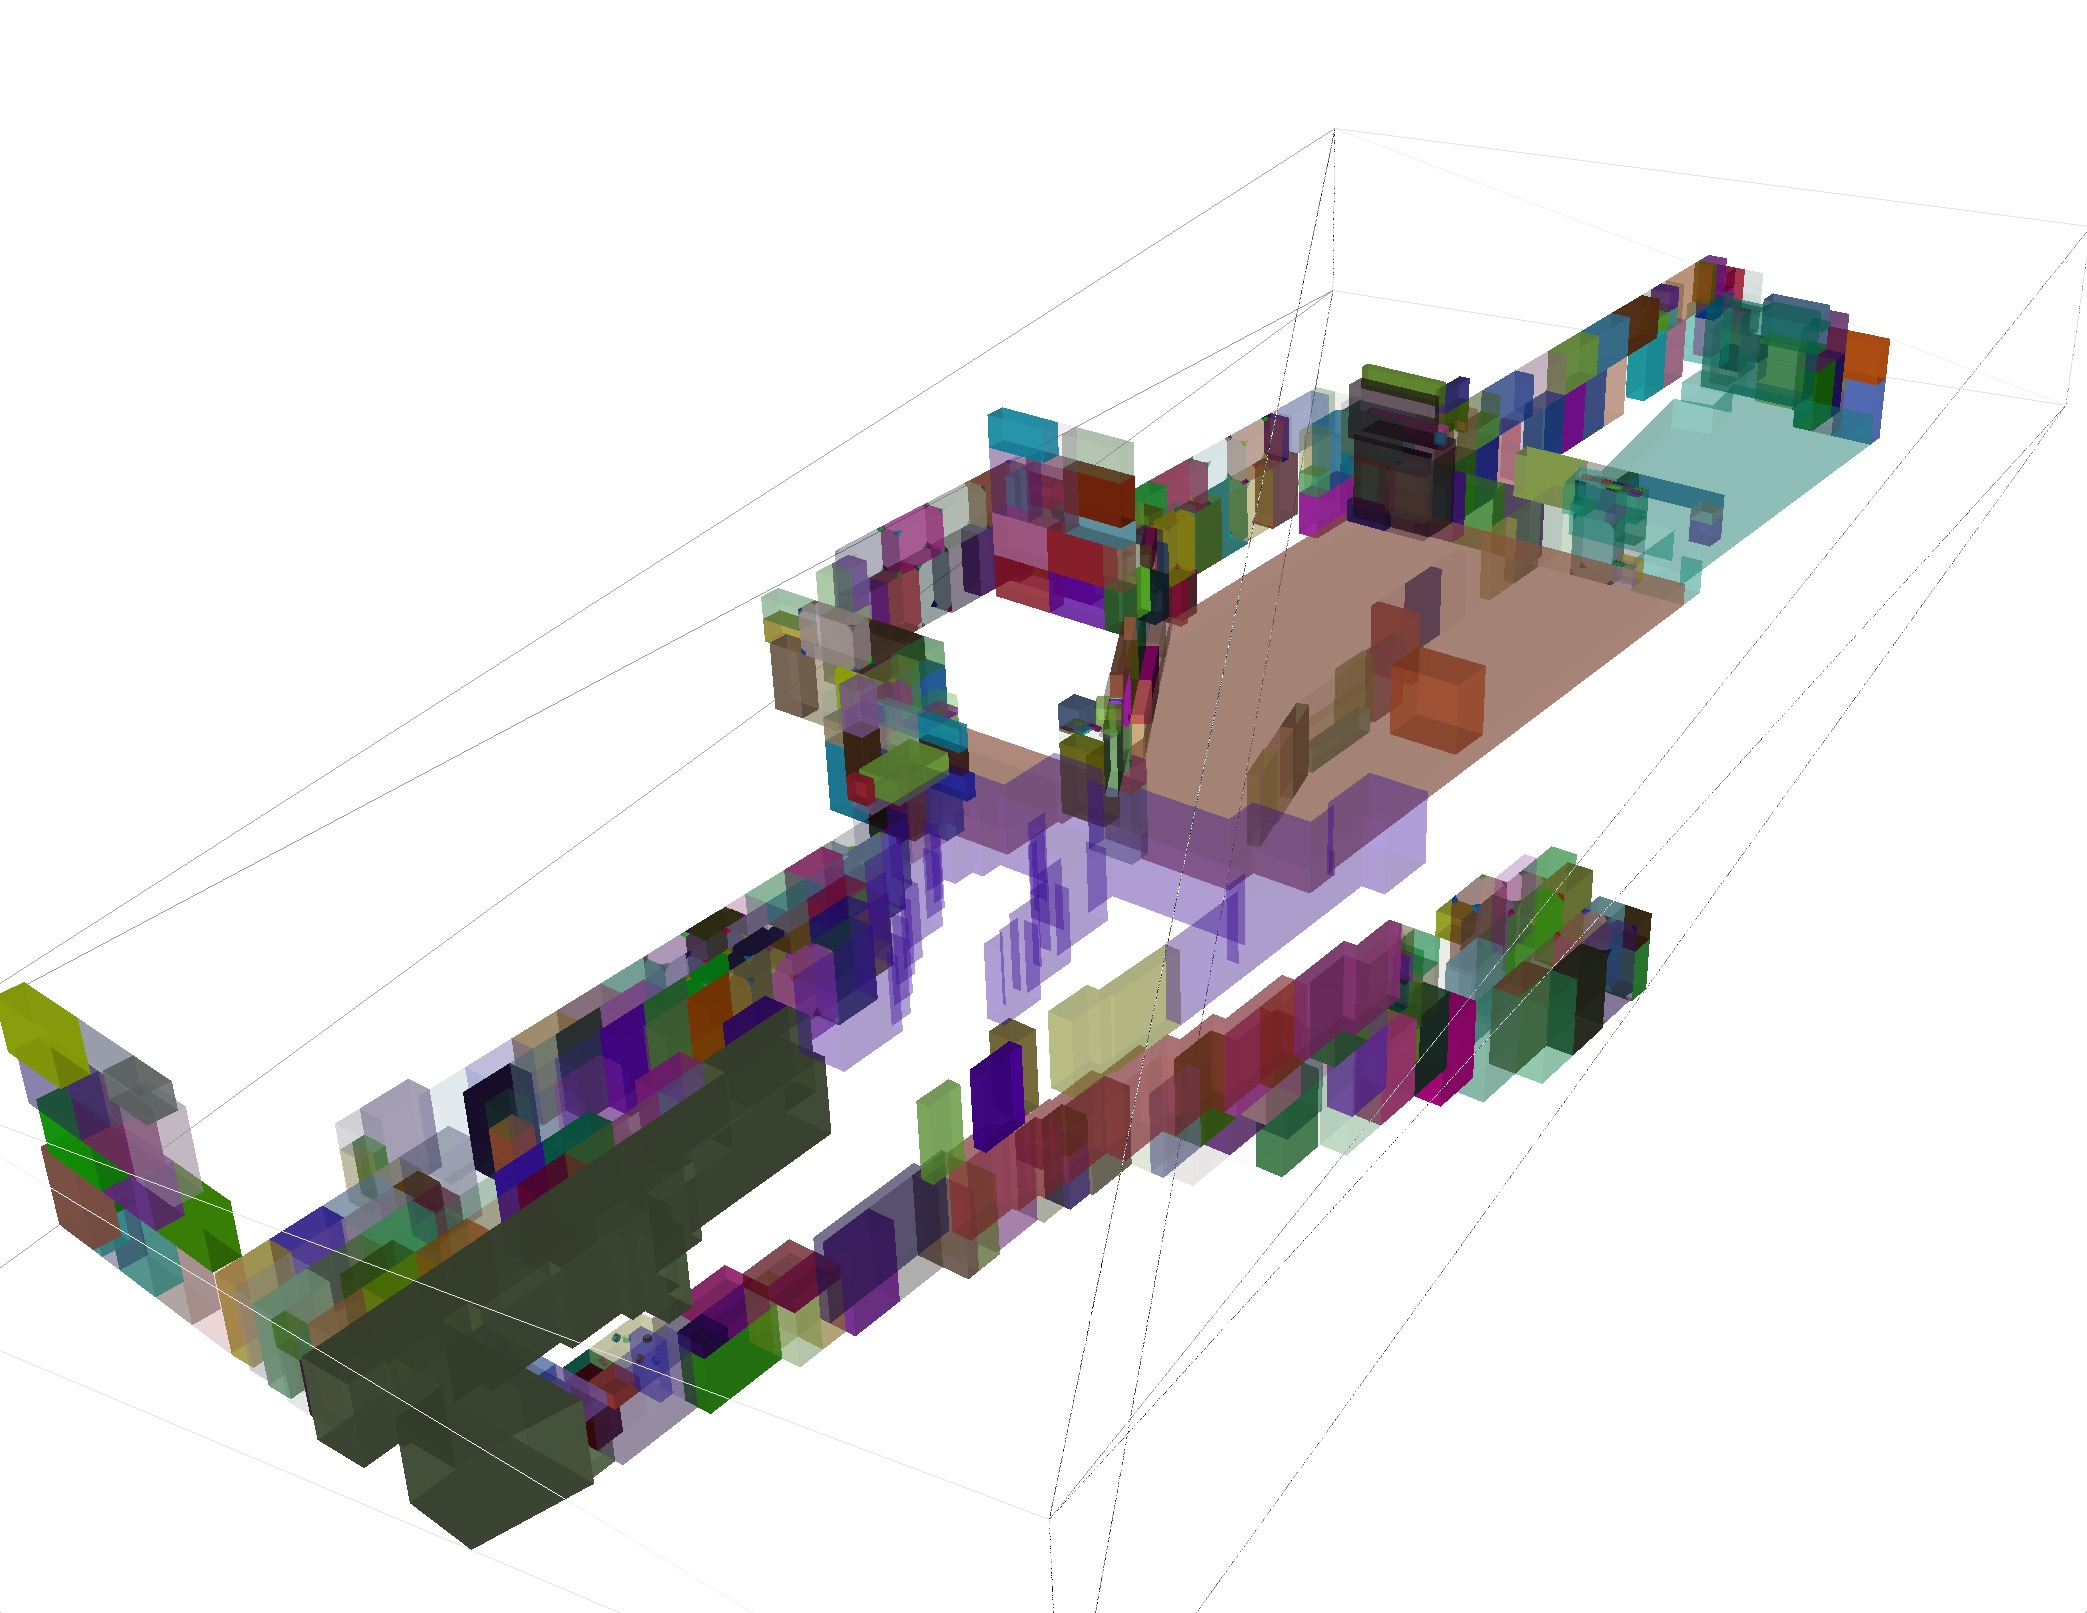
\includegraphics[scale=0.13]{Images//introduction//CernEast.jpg}
\caption[width=\columnwidth]{Converted CAD file (STEP to GDML) of the shielding at CERN East Areas T8 to T11 test beam lines, from Source \cite{pyg4om}.}
\label{cerncad}
\end{figure}

\noindent Figure \ref{cerncad} shows a CAD model of the shielding used in a section of the east area at CERN (or The European Organization for Nuclear Research, translated from French) home to the LHC (or Large Hadron Collider). The use of particle transport simulation can also be used as a tool for simulating beam losses \cite{pyg4om}, which can be applied for experiments such as machine protection, efficiency tests and machine optimisation.

\subsubsection{Space Exploration}
\noindent Space exploration is also a large field where radiation transport and shielding is a key concept that must be accounted for. Beyond the Earth's atmosphere the universe is full of harmful GCR (Galactic Cosmic Rays) radiation and stellar material making the shielding of spacecraft and astronauts a major priority. Traditionally protection against unwanted radiation has involved placing an absorber in between the target and the source. The shielding for a spacecraft is typically made from an aluminum alloy; studies have simulated the effectiveness of $Al_2O_3$ as space craft shielding \cite{spacesh}, taking into account properties of the alloy such as the stopping power. 
\\\\
\noindent However, for the case of astronauts the size of the required absorber is extremely large and impractical and this component will likely cause showers of more harmful secondary radiation. Therefore the use of magnetic fields is being investigated as a way to divert the charged electromagnetic radiation away from a target apposed to stopping it \cite{magf}. This is something which can also be simulated in Monte Carlo software with the inclusion of electric \& magnetic field maps.

\subsubsection{Medical}
\noindent Another essential discipline in which radiation transport simulation is required in is medical treatment. X-ray radiation from vacuum tubes is not only used to check for fractures or breaks in bones, it also used in radiotherapy. The X-rays are used to target unwanted growths in the body through small doses of harmful radiation, with the aim of removing cancerous tissue with minimum damage to the neighbouring organs. This can be especially difficult when the tumor is in the vicinity of organs that move within the body, such as the lungs. As the patient needs to breathe in order to live, the movement of the organs needs to be accounted for when aiming the particles.
\\\\
\begin{figure}[h!]
\centering
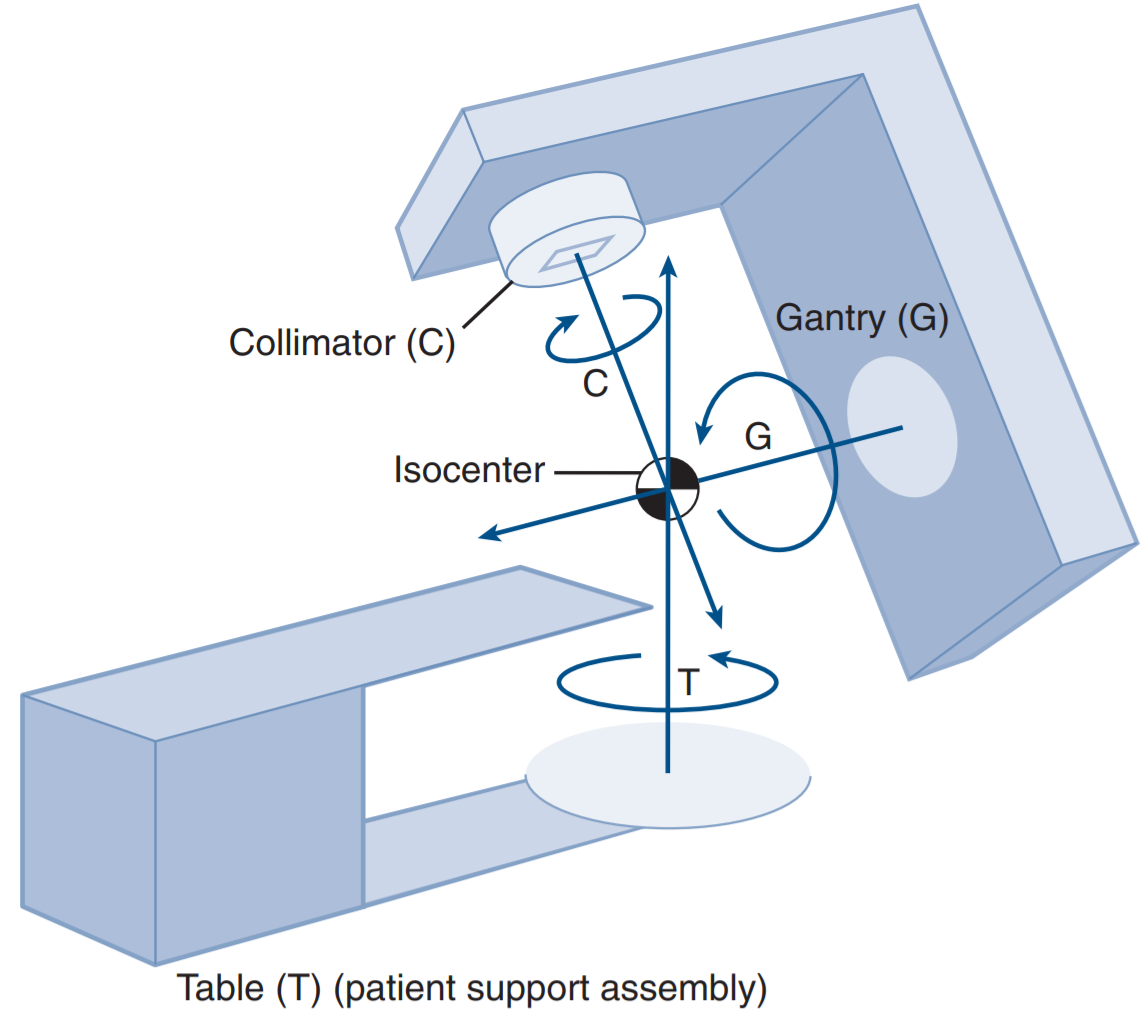
\includegraphics[scale=0.35]{Images//introduction//radiotherapy.png}
\caption[width=\columnwidth]{A gantry-based radiation therapy machine, from Source \cite{cancer}.}
\label{cancer}
\end{figure}

\noindent A patients' organs also move with the body's orientation with respect to gravity therefore the patient must be positioned laying down on a table that rotates perpendicular to the direction of gravity. The gantry unit must then rotate around the patient to imitate the most stationary conditions. An example machine can be seen in Figure \ref{cancer}, where patients would be placed on the table to undergo treatment by radiotherapy; the isocenter being the optimal target position of the cancerous cells to be in within the patents' body.  A more recent type of radiotherapy is proton therapy, which involves the use of small particle accelerators; the use of the word small being relative to size of typical particle accelerators such as the LHC.

% ------------------------------------------------------------------------------------------------------------------------------

\subsection{Project Motivations}
\label{motiv}
\noindent Historically it has been very difficult to simulate particle radiation through matter correctly, being both expensive and time consuming. As computer technology has developed through recent years particle physicists have begun building models to simulate these radiation events, employing techniques such as the Monte Carlo method. Currently many independent industries all require the ability to conduct radiation transport simulations, but use different methodolgies of storing geometries, which come in the form of different file formats. The use of different file formats is where one of the biggest problems lie, as many software tools for simulating radiation transport are format specific and require complex file conversions. 
\\\\
The motivation of the project is to study the efficiency of tessellated solids, where a tessellated solid is a 3D shape whose surfaces are mapped using 2D geometric shapes. Pyg4ometry is a tool created to easily convert between these representations in different formats and allow a wider audience to utilise these radiation tracking softwares. GUImesh is a similar Python package for converting STEP files into GDML format \cite{meh}.

\subsection{Project Aims}
\label{aim}
Simulating radiation transport requires a 3D description of the target formation, detailing its structure, dimensions and material properties such as density. These 3D models contain elements and volumes which can not overlap, leading to most radiation transport geometries being made by hand. These types of aims are possible in software such as Pyg4ometry. The geometries produced in Pyg4ometry can then be simulated in other packages such as BDSIM. The underlying libraries of BDSIM which contribute towards the simulation properties such as the tracking, fields and material physics, arise from GEANT4, which are all discussed in later sections.
\\\\
\noindent The aims of this project are to contribute towards the optimization of the Pyg4ometry package (Section \ref{pyg}) and subsequently BDSIM (Section \ref{bdsim}), by improving parts of the code and conducting performance tests to produce results that can be analysed. The main areas for improvement and where most of the computational energy is wasted is in the meshing of the primitive GEANT4 (Section \ref{g4}) compatible solids. The inefficient computation is primarily due to the unnecessary use of boolean operations (Section \ref{bool}). The first part of the project focuses on the meshing of the primitive solids (Section \ref{prim}) within the Pyg4ometry package, by looking at the comparison of methods and techniques that produce the tessellated meshes. A primitive solid in constructive solid geometry (CSG) is a simple geometric solid such as cube, pyramid, sphere or torus. The second part of the project focuses on the performance of these meshed solids within BDSIM, investigating the effects of material and particle energy on the duration of interactions with the solids.

% ------------------------------------------------------------------------------------------------------------------------------

\section{Software Packages}
\label{packs}
This section outlines the key details of each package, describing its function and link to the project. At the time of the project a lot of the prerequisite packages were only compatible with Linux Operating Systems (OS) and no docker images were available. Due to owning a machine that operated on Microsoft Windows, the project was then completed on a Linux laptop (a 2011 Apple MacBook Pro running OS X 10.11 El Capitan) from the RHUL Physics Department. The setting up of virtual machines running Cent0s 7 (standard free Linux OS used by CERN \cite{cern}) was also attempted, however despite getting it successfully setup, the packages were not performing to the same standard as they were on the fellow Apple MacBooks. This legacy OS on the loaned laptop came pre-installed with the some of the required packages, and allowed for easy installation of outstanding backdated versions. 


%========================================================================================

\subsection{GEANT4}\label{GEANT4}
\label{g4}
GEANT4 (or GEometry ANd Tracking) \cite{geant} is a toolkit developed in C++ for the simulation and tracking of particles traveling through matter by employing the Monte Carlo method (Section \ref{monte}). It is used by many particle physicists and is one of the more popular packages used to create 3D models of experiments for Monte Carlo simulations. GEANT4 has its own preset primitive solids that are used for simulating particle interactions and can be found within the online manual \cite{g4man}. The naming convention of the solids being used in this project and within this report are the ones used by GEANT4. GEANT4 also has a large inbuilt database which contains the properties of most materials and particles. An alternative transport code is FLUKA (or FLUktuierende KAskade) \cite{fluka}, which also uses Monte Carlo to simulate high energy physics. GEANT4 has also been used to conduct dose calculations for radiotherapy patients \cite{dose} as well as many other simulations around particle losses and background radiation \cite{will}. The materials used throughout this project are from the GEANT4 database, which can also be found listed in the manual \cite{g4man}. In this report the three main materials used are Tungsten, Titanium and vacuum (G4\_W, G4\_Ti and G4\_Galactic). The use of G4\_Galactic is arguably the most important as it is used to set the material of the world environment in which other objects are placed into.

%========================================================================================

\subsection{BDSIM}
\label{bdsim}
% ref another bdsim papere saying em fields to fully transport partiles in start to end simulations of particle accelerators (before GMAD bit)


BDSIM (or Beam Delivery SIMulation) \cite{bdsimpap} is an open-source software package also written by JAI (John Adams Institute) at Royal Holloway for the use of modelling particle beam interactions. The package is written in C++ and has many applications, such as modelling complex particle accelerators like the Large Hadron Collider (LHC) or low energy magnetic beamlines for radiotherapy applications used to treat tumours. BDSIM allows a user to specify the physics being used for a particular particle interaction, such as the particle energy and the number of secondaries produced. BDSIM works by intaking a simple ASCII file with its own extension (GMAD), where the simulation and model can then be controlled by the GMAD's parameters. One of these parameters is the ``worldMaterial'', which defines the material of the environment that other elements and volumes are placed into. By default, the world material in BDSIM is set to be air, which means the particles would interact before passing into the object being tested; this can be avoided by using the option $worldMaterial=``G4\_Galactic"$ within the GMAD files, where G4\_Galactic is the GEANT4 vacuum material as mentioned before (Section \ref{bdsim}). Other properties for each GEANT4 material are also used in this project, such as the stopping power (Section \ref{stop}).
\\\\
Although the BDSIM's defaults build up a standard geometry beamline, often specialised pieces of geometry are needed to accurately simulate interactions; this can be done by supplying an external GDML file, where its placement in the simulation can be specified in the GMAD. The scattering of the particle trajectories and decays are computed using Geant4's Monte Carlo calculations, to make the results as consistent with experimental data as possible. The software outputs a ROOT file contain all the required information. As many particles as desired can be simulated in batch mode, however a GUI is available to view the geometry, but is rarely used to simulate the particle accelerators as it is computationally expensive. 
\\\\
Inside the 3D interactive environment within the GUI, BDSIM uses the discrete colouring convention of tracks to represent a particles charge inherited from GEANT4, where a green track is neutral, blue is positive and red is negative, which can be seen in Figures throughout this paper. The option ``physicsList'' defines the physics which is used for the interaction, for the project the option was set to``g4FTFP\_BERT'', which contains all the standard electromagnetism and particle physics required for this project. The physics can be used to chose the desired types of radiation emission and interactions taken into account for a given event. The outputted ROOT files contain a detailed analysis of the interaction. One of the elements analysed within this project is the CPU duration time distribution of an interaction in BDSIM.

\subsubsection{Pybdsim}
\label{pyb}
BDSIM has a Python utility library called Pybdsim which provides an interface to be automate BDSIM and read its output files for data processing using Python scripts. Pybdsim also allows for the navigation of ROOT analysis files to extract data to plot, mentioned further in Section \ref{root}. This is how all the plots in Sections \ref{prim} \& \ref{int} are generated.


%=========================================================================================

\subsection{Pyg4ometry}
\label{pyg}
Pyg4ometry is an open-source Python package, developed by the John Adams Institute at Royal Holloway \cite{jai}; its purpose is to convert 3D CAD (Computer Aided Design) geometries between different representations to allow compatibility with BDSIM (Section \ref{bdsim}) for the simulation of radiation transport \cite{pyg4om}. The ``4'' in ``Pyg4ometry'' comes from the fact Pyg4ometry has been written to design geometries specifically for GEANT4 (Section \ref{GEANT4}). The package is a key tool for allowing multiple file formats, such as STEP/STL or IGES files to be converted into GDML files, which are the compatible format for BDSIM. GDML (or Geometry Description Markup Language) is a format based on a XML file type. The range of file compatibility increases the number of people who can utilise both Pyg4ometry and BDSIM, as many industries use different file formats to store their 3D CAD geometries.
\\\\
\noindent Pyg4ometry can also be used to determine if a model has any geometric overlap and provides faster loading for CAD geometries into BDSIM compared with the full GEANT4 C++ application. Most of the development in this project is conducted in Pyg4ometry. As of January 2020 the first CentOs 7 docker image for Pyg4ometry is now available in the source code repository. The package is currently written in and only supports Python 2.7, however as of January 2020 developer support for Python 2 has been discontinued as the newer version Python 3 is taking over. The transition to Python 3 means adjusting the syntax of several functions and files in Pyg4ometry, this has begun, however a full transition will take sometime as it is not an immediate priority. 

\subsection{ROOT}\label{root}
ROOT is not an acronym and is named after the idea, that it is a system for other systems to grow off of, much like a root of a tree that has many branches. ROOT is adopted by many physics communities such as CERN \cite{cern}, where it was first written, naturally making it a popular format for particle physicists in particular and is the why it is the default output for analysis by BDSIM. Despite ROOT storing data in the format of its own plots, no ROOT files or plots are shown in the report, as the data has been extracted from the root files and replotted using Pybdsim \ref{pyb} and Matplotlib. The plots are made this way as the data can be more easily manipulated and the formatting of ROOT plots is more complex than with a simple Python script, of which a few standardised examples are used in Pybdsim.

\subsection{FreeCAD}
In this report the libraries from FreeCAD 0.18 \cite{18} are used directly within Pyg4ometry (Section \ref{pyg}), without the use of the FreeCAD Graphical User Interface (GUI). The libraries are used to import STEP files and to convert them into triangular based tessellated meshed solids, that can then be written out as a GDML file. As an exercise at the beginning of the project a few example CAD STEP files were downloaded from the Internet and converted into meshed GDML files. One of the CAD models converted was a GPS satellite, which can be seen in Figure\ref{sat}. FreeCAD itself can also be used to create CAD models that can then be tested in BDSIM, an example magnet shown in Appendix \ref{mag}.

\subsection{Visualisation}
\label{vis}
Most of the packages mentioned above have their own GUIs to visualise the meshed geometries. However the main two GUIs used in this project are the ones used by Pyg4ometry and BDSIM. VTK (or Visualization ToolKit) is an open-source software for displaying and manipulating scientific data \cite{vtk}. Pyg4ometry uses VTK, shown in Figure \ref{sat}, to create its 3D interactive GUI. BDSIM uses GEANT4's GUI (as seen in Figure \ref{screengrab}), which is another reason Pyg4ometry aims to be consistent with GEANT4. Both the VTK and GEANT4 GUI's allow meshed solids to be viewed as solids or as meshed structures. The GEANT4 GUI has its own console in which commands can be carried out, allowing the simulation to be altered from within the GUI as well as by Pybdsim.

\begin{figure}[h!]
\centering
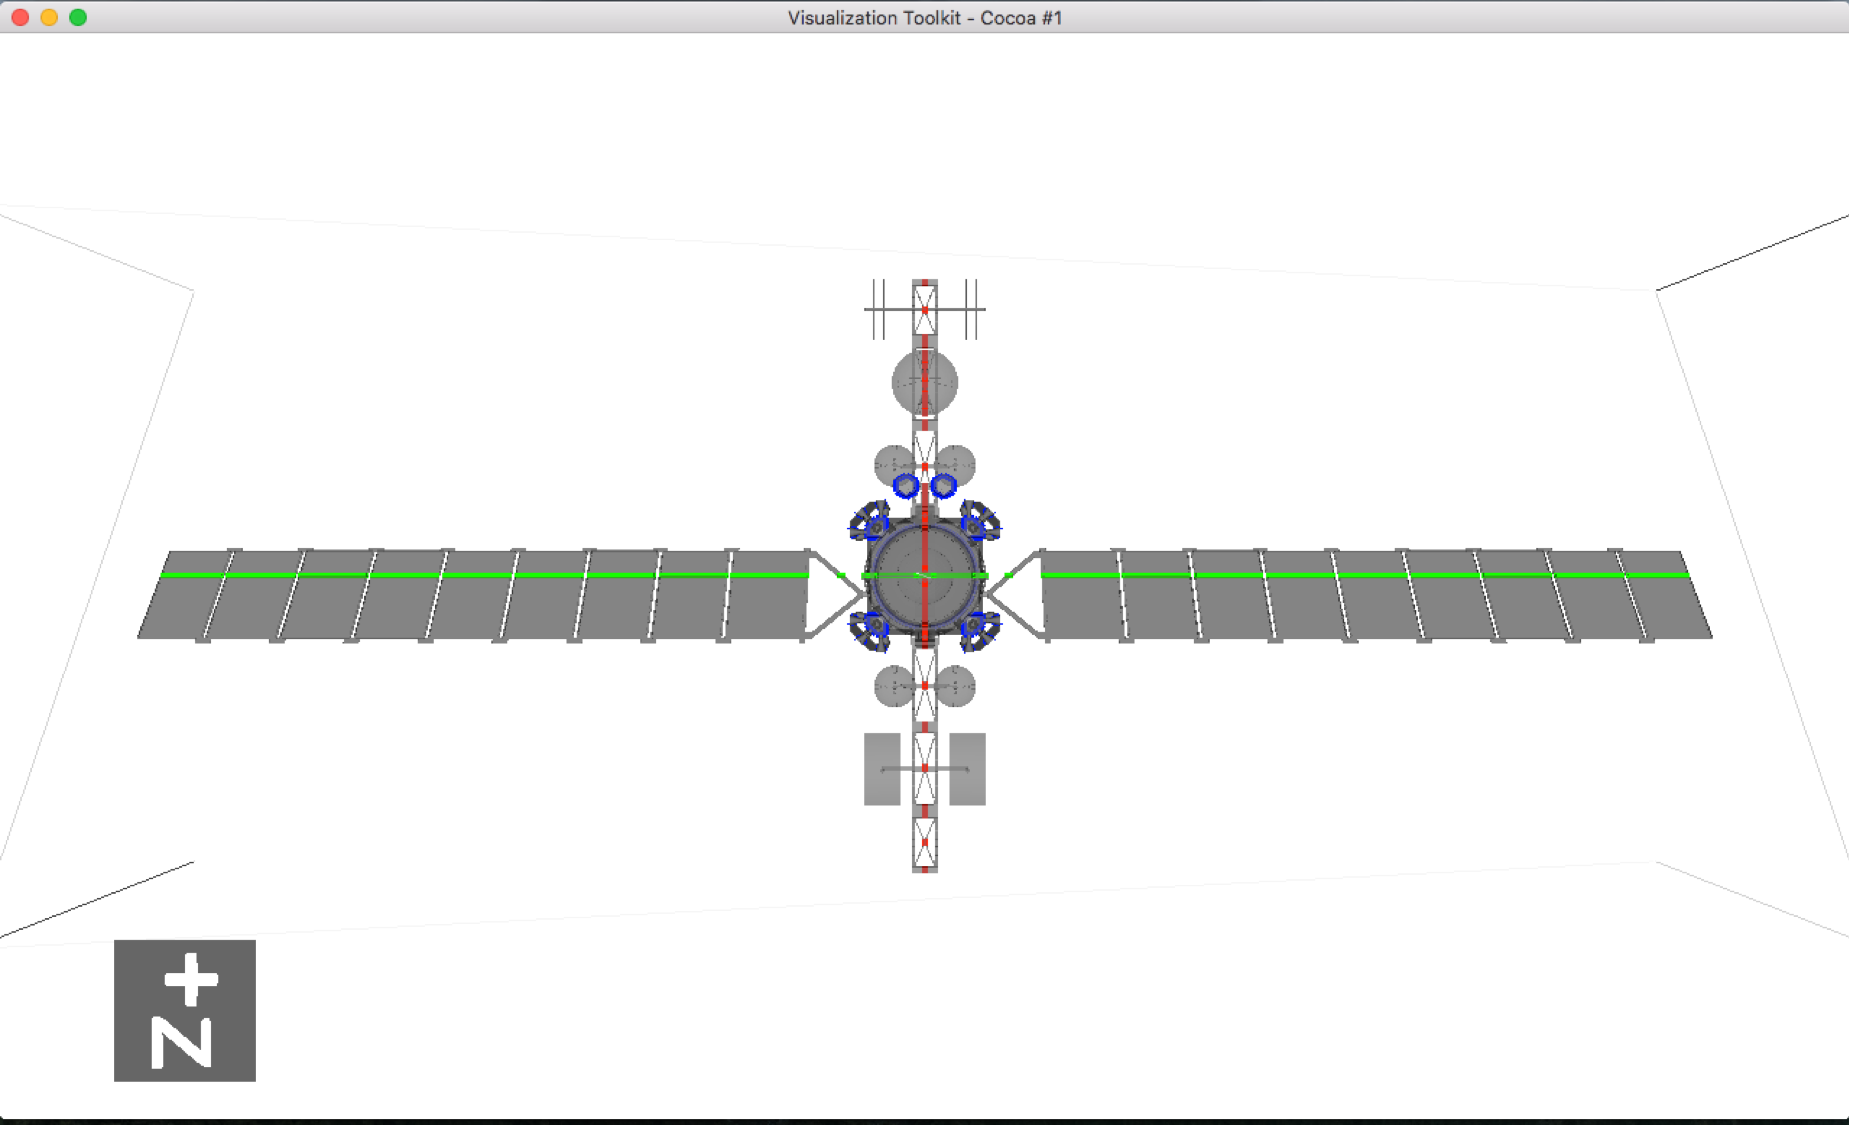
\includegraphics[scale=0.4]{Images//VTK/sat.png}
\caption[width=\columnwidth]{STEP file of a GPS satellite imported into Pyg4ometry using the FreeCAD libraries and viewed in VTK. Original STEP file from Source \cite{sat}.}
\label{sat}
\end{figure}

\begin{figure}[h!]
\centering
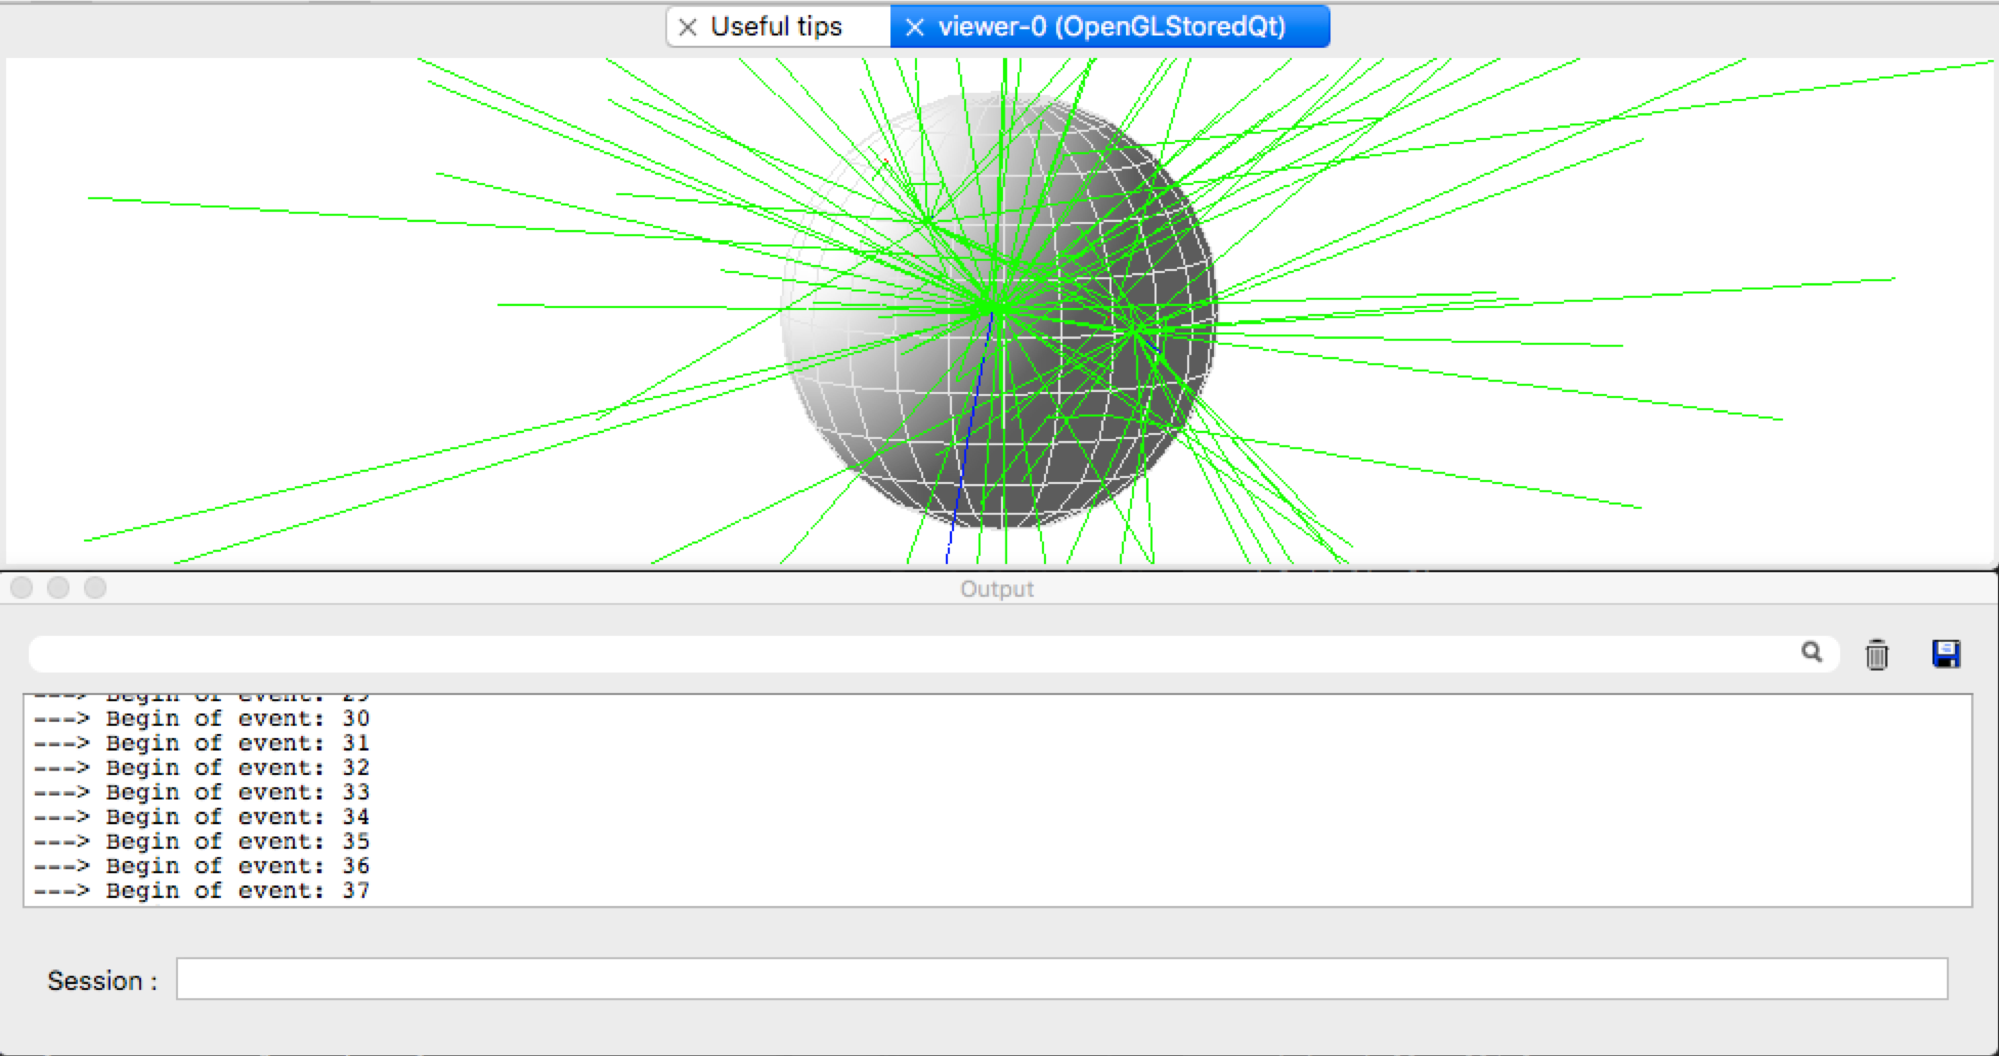
\includegraphics[scale=0.4]{Images//BDSIM//screengrab.png}
\caption[width=\columnwidth]{BDSIM GUI screenshot of a 3D particle interaction and output window, showing a GEANT4 Sphere with 100 1.3 GeV neutrons.}
\label{screengrab}
\end{figure}

% -----------------------------------------------------------------------------------------------------------------------------

\newpage
\section{Primitive Meshing}
\label{prim}

This section will describe the work done to optimize the Python scripts that generate the three dimensional meshings for the primitive solids within the Pyg4ometry package (Section \ref{pyg}). All the primitive solids used are constructed such that they are compatible with GEANT4's solids \cite{solids}. It was previously thought that it would be best to use purely triangular based meshes in combination with boolean operations to construct the 3D solids. The triangle is the shape which has the minimum amount of points needed to define a planar face containing an area. Prior to the project it had been realised that the computation of triangles and boolean operations in most cases is much more intensive and inefficient, compared with the polygons and adapted trigonometry. In particular with the curved solids are the most computationally heavy, i.e cylindrical, spherical and toroidal based solids, due to the boolean operations generating more complex meshes. Thus the first part of the major project was to rewrite the meshing scripts for all the curved primitive solids in Pyg4ometry (Section\ref{pyg}).
\\\\
One of the major improvements to the Pyg4ometry meshing scripts was in the computation of sectioned primitive solids. The meshing of hollow or sliced solids were previously constructed by boolean subtractions and intersections, which involves using two or more separate solids and operating on them to create a final single solid. This resulted in a very computationally heavy and less aesthetic outcome, where the mesh lines (``slice and stack'') were often meshed in non-axial directions.

\subsection{Co-ordinate Systems}
\label{cosy}
The various primitive solids are all constructed by using the predefined parameters used by GEANT4, to be consistent with GEANT4's own convention for solids. The parameters defining a 3D solid are properties relating to the co-ordinate system that the solid is constructed within. For example for a simple cylinder the parameters would be a height and radius. The parameters are then used to generate points on the object via basic trigonometry. The points can then be used as vertexes to define faces on the given solid. The number of faces and subsequently the number of points on a solid's surface defines the mesh density. The order in which the points are appended is also very important and is detailed in Section \ref{order}.
\\\\

\begin{lstlisting}[language=Python, label=code1, caption=Basic Python function structure for new meshing of primitive solid in Pyg4ometry.]
def pycsgmesh(nslice,nstack, *args, **kwargs):

    # ... 
    
    polygons = []

    for j0 in range(nslice):
        j1 = j0
        j2 = j0 + 1
    
        vertices = []

        for i0 in range(nstack):
              i1 = i0
              i2 = i0 + 1     
              
    #....
    
    return mesh

\end{lstlisting}

\noindent The Python meshing scripts for all co-ordinate systems follow a similar structure, using a pycsgmesh function, the beginning of which can be seen in Listing \ref{code1}. The ``CSG'' in ``pycsg'' stands for Constructive Solid Geometry, which is a modelling technique that uses boolean operations to construct 3D solids. The naming convention is left over from when the old meshing scripts employed boolean operations. The script works by first defining an empty list of faces (polygons) and then running the associated trigonometric equations through a number of loops to generate and append polygons to that list. The number of loops is defined with the number of sections a surface of a solid is being split up into in a given co-ordinate system (``nslice'' \& ``nstack'' in Listing \ref{code1}). The two parts of Listing \ref{code1} where code has been commented out is where a lot of repetitive code is placed. The first comment block is where the units and other empty lists are defined and the second is were all the points, faces and polygons are constructed using ``pycsg.geom'' functions. The density of the mesh is defined by the function arguments supplied by the user for the number of slices and stacks, of which the orientation varies with co-ordinate system. The slice and stack used by the new meshing scripts for the solids in the cylindrical polar, spherical \& toroidal co-ordinate systems are detailed in the following Sections \ref{cycl}, \ref{sphh} \& \ref{too}.

\subsubsection{Cylindrical Polar Co-ordinate System}
\label{cycl}
In the cylindrical polar co-ordinate system the loops within the equivalent function to Listing \ref{code1} creates 3 or 4 points at a time using an adaptation to the trigonometry in Equation \ref{cyctrig}, which can then be used to define a triangular or quadrilateral face. The only cases where the new meshing produces triangles is at the top and bottom faces of the cylinder, as shown in Figure \ref{cylmeshin}. These cases are only true provided the solid does not have a minimum radius equal to zero (creating a tube or cone). The same logic for the triangular faces is identical to that of the quadrilateral faces, just using 3 vertex points to make a face.

\begin{figure}[h!]
\centering
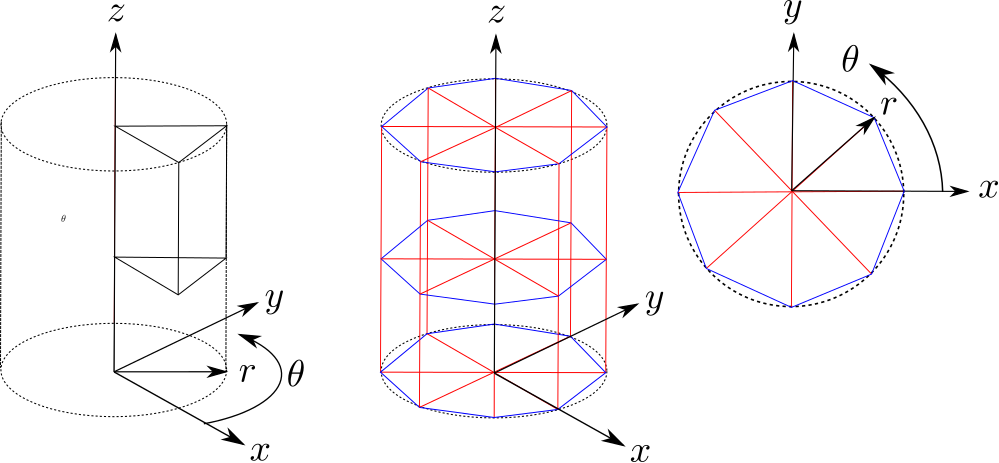
\includegraphics[scale=0.45]{Images//Coords//cyl.png}
\caption[width=\columnwidth]{A diagram showing the meshing method for a cylindrical polar co-ordinate system, where the red lines indicate the slices (8) and the blue indicate the stacks (2). The far left diagram depicts a single face in the co-ordinate system using two slices and two stacks to define its four vertexes. The middle diagram shows a complete view of a constructed mesh, using both slice and stack. The far right diagram depicts the meshed cylinder in the x-y plane (top view), to further illustrate the the slice is taken radially.}
\label{cylmeshin}
\end{figure}
The trigonometry that converts the points from cylindrical polar co-ordinates to Cartesian are:
\begin{equation}
\begin{aligned}
\label{cyctrig}
& x = r \cos{\theta} \\
& y = r \sin{\theta} \\
& z = z
\end{aligned}
\end{equation}

\noindent The only time a stack is needed in the cylindrical co-ordinate system is when the solid has a non-linear function in the r-z plane. For example, a Paraboloid (Figure \ref{paraco}) would need a stack, but a linear cone (Figure \ref{consco}) would not. This is due to the fact that a singular plane can not represent a curved surface with a one face. 

\begin{figure}[h!]
\centering
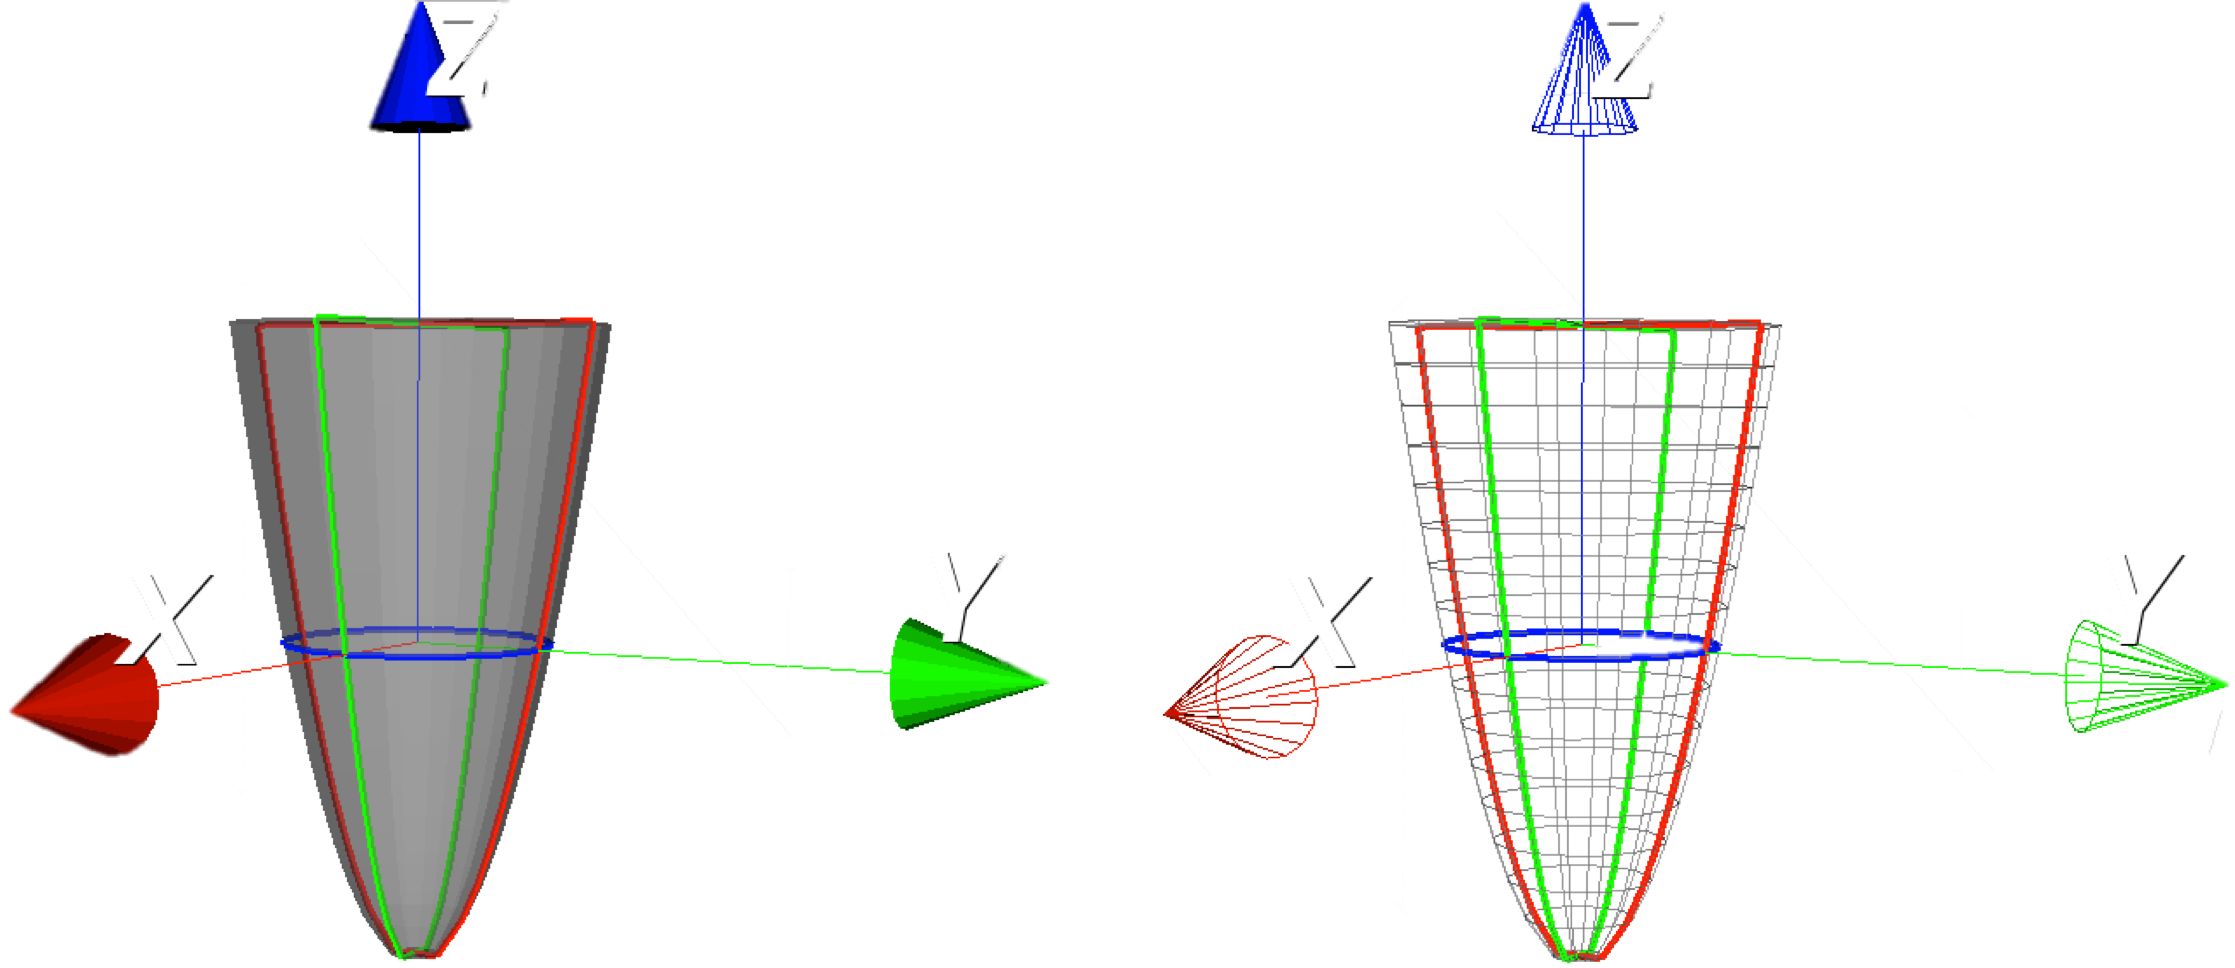
\includegraphics[scale=0.3]{Images//Coords//para.png}
\caption[width=\columnwidth]{A Paraboloid constructed using the new meshing method in cylindrical polar co-ordinate system, where the red lines indicate the points residing on the x=0 plane, the blue lines indicate points on the z=0 plane and green lines indicate points on the y=0 plane.}
\label{paraco}
\end{figure}

\begin{figure}[h!]
\centering
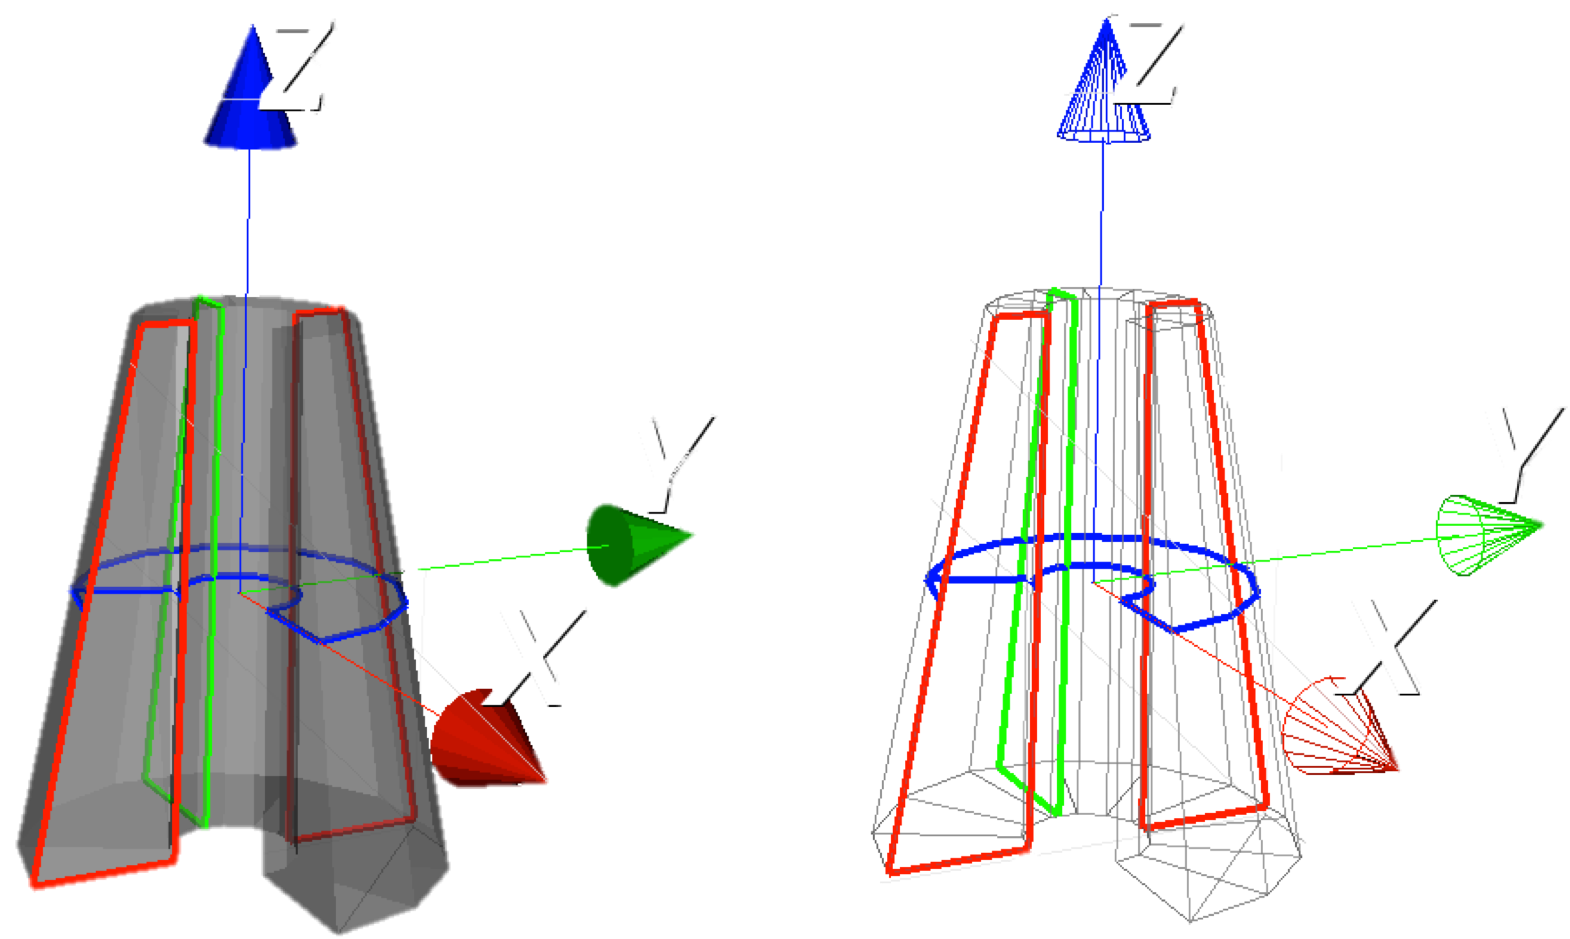
\includegraphics[scale=0.3]{Images//Coords//consco.png}
\caption[width=\columnwidth]{A Cons (hollow cone) constructed using the new meshing method in cylindrical polar co-ordinate system, where the red lines indicate the points residing on the x=0 plane, the blue lines indicate points on the z=0 plane and green lines indicate points on the y=0 plane.}
\label{consco}
\end{figure}

\newpage
\subsubsection{Spherical Co-ordinate System}\label{sphh}
The meshing for the primitive solids in spherical co-ordinate systems are constructed by similar means to that of the cylindrical co-ordinate system, with different trigonometric equations (Equation \ref{trigsph}) as a result of two angle parameters $\phi$ and $\theta$. The stack (blue) and slice (red) for solids in the spherical co-ordinate system works in the same way as the longitudinal and latitudinal mapping on a globe, shown in Figure\ref{sphmeshin}. 
\\\\
The trigonometry that converts the points from spherical co-ordinates to Cartesian are:

\begin{equation}
\begin{aligned}
& x = r \cos{\theta}\sin{\phi}\\
& y = r \sin{\theta}\sin{\phi} \\
& z = z
\end{aligned}
\label{trigsph}
\end{equation}
\begin{figure}[h!]
\centering
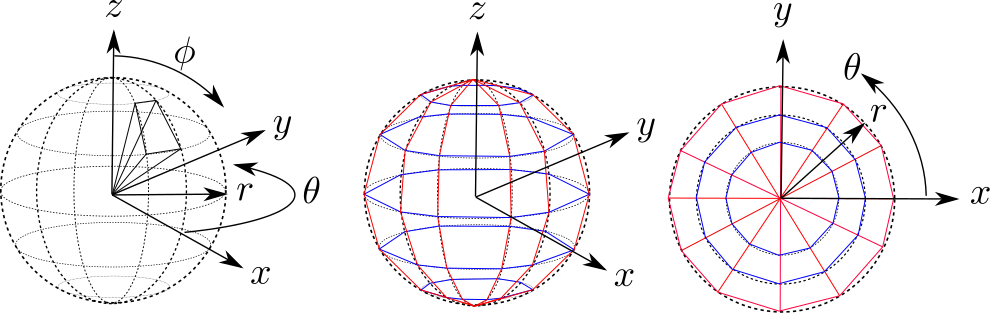
\includegraphics[scale=0.5]{Images//Coords//sph.png}
\caption[width=\columnwidth]{The meshing method for a spherical co-ordinate system, where the red lines indicate the slices (12) and the blue indicate the stacks (6). The far left diagram depicts a single face in the co-ordinate system using two slices and two stacks to define its four vertexes. The centre diagram depicts a fully meshed Orb made out of both stack and slice. The far right diagram shows the meshed Orb in the x-y plane (top view), to further illustrate the the slice is taken radially and that the stacks are circular in nature.}
\label{sphmeshin}
\end{figure}

\noindent The structure of the code for a spherical co-ordinate system is the same as used in Listing \ref{code1}. The only time triangles are constructed in the spherical co-ordinate system is if a complete pole exists at the top or bottom of the solid. The solids constructed in the spherical co-ordinate system always have both a stack and a slice.

\newpage
\subsubsection{Toroidal Co-ordinate System}
\label{too}
The toroidal co-ordinate system is a special case and is only needed for toroidal based solids. The stack and slice for a toroidal shape is much more complex to visualise, due to the fact it is a rotating co-ordinate system. A toroidal slice is an $R_{Torus}$ radial cut taken out of the angle $\phi$ and a toroidal stack is a $R$ radial cut out of the angle $\theta$, where the angles and radii are displayed in Figure\ref{tormeshin}. 
\\\\
The trigonometry that converts the points from toroidal co-ordinates to Cartesian are:

\begin{equation}
\begin{aligned}
& x = R_{Torus} + R\cos{\theta}\cos{\phi} \\
& y = R_{Torus} + R\cos{\theta}\sin{\phi} \\
& z =  R\sin{\theta} 
\end{aligned}
\end{equation}

\begin{figure}[h!]
\centering
\includegraphics[scale=0.35]{Images//Coords/torus_coords.png}
\caption[width=\columnwidth]{Diagram showing the meshing method for a toroidal co-ordinate system. The far left diagram shows a section of a toroidal slice, where the slices are being cut radially in the $\phi_1$ direction. The centre diagram depicts a full un-meshed torus, with an outlined ring residing on the surface of the torus of radius R. The far right diagram shows how the different radii of the torus have been define in the meshing script.}
\label{tormeshin}
\end{figure}

\subsection{Plane Direction}
\label{order}
A key consideration when writing Pyg4ometry meshing scripts is the order convention being used for appending points/vertexes to a list, to define a plane, i.e to define a face on a solid. This is important as the direction the normal of the plane points in, dictates whether a face is considered an inside or outside face on the given solid. Getting this order incorrect will lead to missing faces when the meshing is made.
\begin{figure}[h!]
\centering
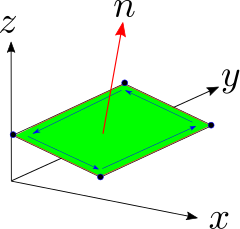
\includegraphics[scale=0.7]{Images//append_points//Point_Appending_Order.png}
\caption[width=\columnwidth]{The order convention of appending points to define the normal to a plane in the Pyg4ometry package.}
\label{pointsorder}
\end{figure}
\noindent The convention is that the normal to a plane points away from the solids surface, making it an exterior face. The normal is in the z direction to a plane residing on z=0, if the points are appended anticlockwise in the x-y plane. For points appending in the other direction (clockwise in the x-y plane), the normal would be in the -z direction, making an interior face. The concept is shown in Figure \ref{pointsorder}.
\\\\
The simplest way to test this is by performing boolean operations with a solid box, as the boolean operation will only work correctly if all the planes are correct on both shapes, mentioned in more detail in Section \ref{bool}. This test only works for the visualiser in BDSIM as it uses GEANT4, which displays face directions. VTK inside Pyg4ometry is a much more lenient visualiser and will display solids even if their normals are incorrect, giving the user a false perspective of what is being displayed. These tests are shown in subsequent Section \ref{bool}.

\subsection{New Meshing of Curved Primitive Solids}
In total there are 12 curved primitive solids, of which many of the examples and concepts are very similar. Therefore only a few select solids will be discussed in this section, but the remaining solids and their development can all be viewed in Appendix \ref{poy}.
\\\\
One of the curved solids for which the meshing was rewritten is the Hyperboloid, the old and new meshing structures of the Hyperboloid is shown in Figure\ref{polypic1}. It can be seen that in this example the meshing at the top and bottom faces becomes more radially uniform. This is due to the replacement of boolean subtractions with simple trigonometry within the new meshing algorithm for the Hyperboloid.
\\\\

\begin{figure}[h!]
\centering
\begin{minipage}{.4\textwidth}
  \centering
  \includegraphics[height=1\linewidth]{Images//Meshes//Hyperboloid.png}
  \captionof{figure}{VTK screenshots of\\ Hyperboloid meshing Development\\ (Solid \& Mesh View)}
  \label{polypic1}
\end{minipage}%
\hspace{1mm}
\begin{minipage}{.4\textwidth}
  \centering
  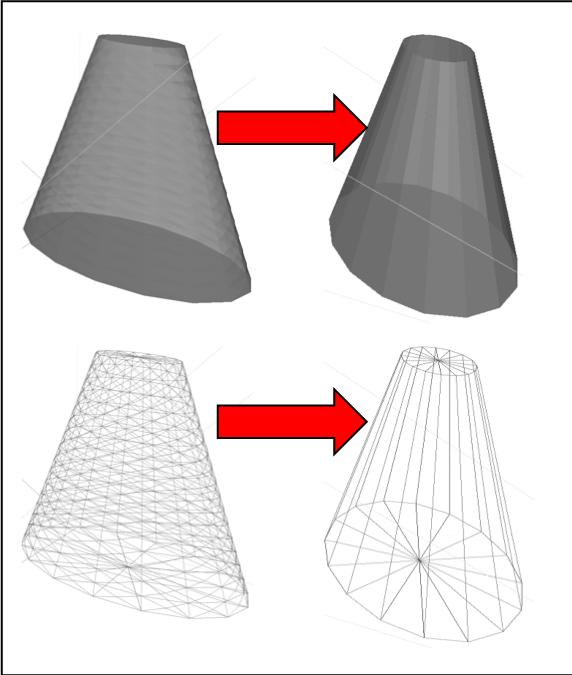
\includegraphics[height=1\linewidth]{Images//Meshes//ellipticalcone.png}
  \captionof{figure}{VTK screenshots of\\ Ellipticalcone meshing Development\\ (Solid \& Mesh View)}
  \label{elco1}
\end{minipage}%
\end{figure}

\noindent Another curved solid that was remeshed is the Ellipticalcone, as seen in Figure \ref{elco1}. Despite having no boolean operations to generate this solid, the meshing is still improved by replacing all the unnecessary triangular faces with quadrilateral ones. For the Ellipticalcone it was also possible for the stack to be removed, as for a cone the faces in the r-z plane (in cylindrical co-ordinates) are a linear function.
\\\\
\noindent A feature that is also removed by the transition to the new meshing algorithms is the "grenade like" texture seen on the surfaces of the curved solids. The clearest example being the Ellipsoid, shown in Figure \ref{ellipme}, where it can be seen that the surface of the solid has not only become triangulated, but also has a contour. This is due to the fact that the old mesh would tend to use quadrilateral based pyramids instead of quadrilateral faces in attempt to better estimate a true curved solid. This was done by rotating every other stack to be out of phase when appending vertexes. Despite this improving the mesh accuracy, it was removed as when one increases the orders of stack and slice to high enough orders the difference is negligible and is not worth the extra computation.  The old meshing for CutTubs as seen in Figure \ref{ct}, had some strange deformations appear at some stage throughout the course of project, which is believed to be related to the slicing of the ends via boolean operations, however there is no point in spending time fixing code that has already been replaced.

\begin{figure}[h!]
\centering
\begin{minipage}{.4\textwidth}
  \centering
  \includegraphics[height=1\linewidth]{Images//Meshes//Ellipsoid.png}
  \captionof{figure}{VTK screenshots of\\ Ellipsoid meshing Development\\ (Solid \& Mesh View)}
  \label{ellipme}
\end{minipage}%
\begin{minipage}{.4\textwidth}
  \centering
  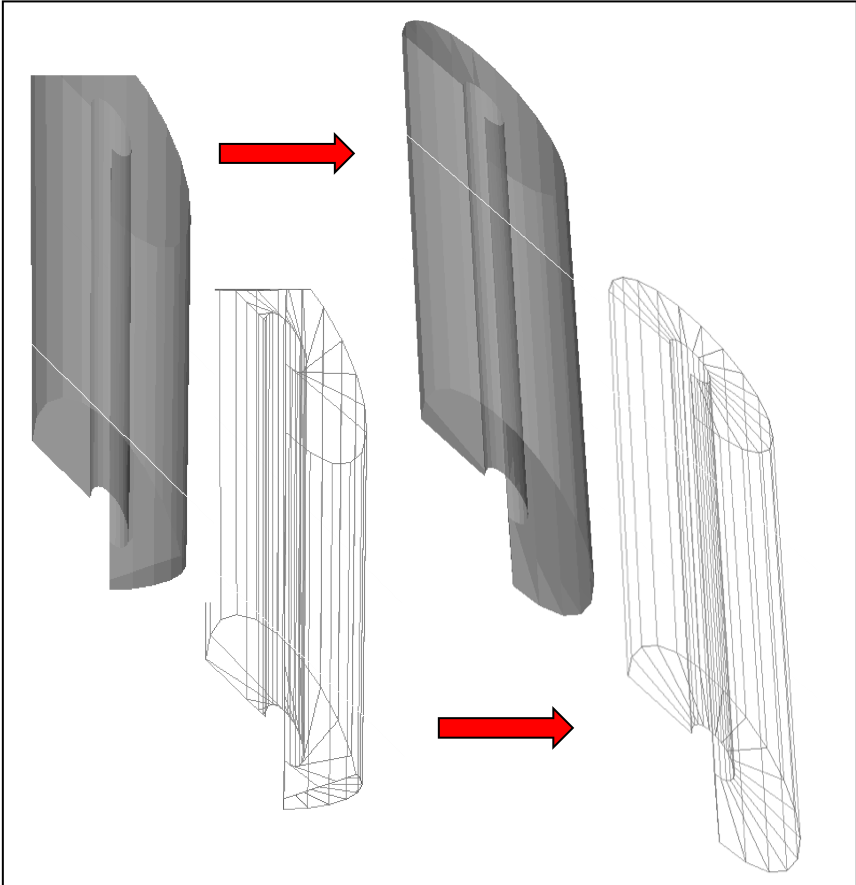
\includegraphics[height=1\linewidth]{Images//Meshes//CutTubs.png}
  \captionof{figure}{VTK screenshots of\\ CutTubs meshing Development\\ (Solid \& Mesh View)}
  \label{ct}
\end{minipage}%
\end{figure}

\subsubsection{Degenerate Points}
Degenerate points are a common mistake which can cause missing faces to occur, due to creating a face with null area. Multiple meshing points occupying the same point in space can spring a few errors, sometimes without entirely crashing the meshing script, making it a potentially hard error to identify. It is typically given away when a $DivisionByZero$ error occurs, within the pycsg meshing of a solid. One can identify whether this is the error by debugging each polygon in a mesh, looking out for a face that has two or more vertices with the same $(x,y,z)$ coordinates. This typically happens when a triangle is intend to be meshed, but are still using the format for meshing a quadrilateral face. Or it can be due to the choice of an incorrect stack and slice iteration when constructing a face, as mentioned before in Section \ref{cosy}.

\subsubsection{Boolean Operations}
\label{bool}

\begin{figure}[h!]
\centering
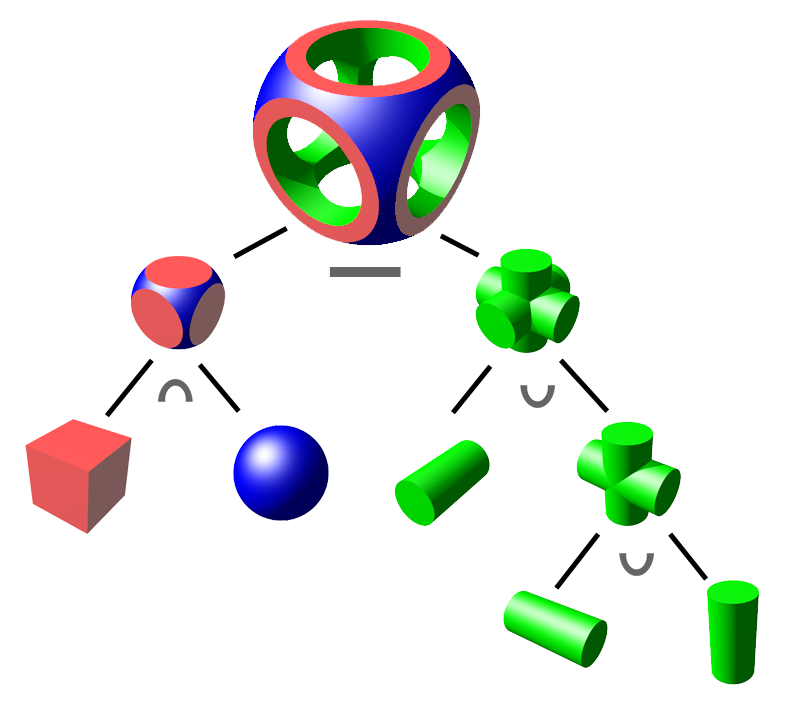
\includegraphics[scale=0.25]{Images//Booleans//Boolean.png}
\caption[width=\columnwidth]{An example CSG solid showing the basic method of constructing a more complicated 3D solid using boolean operations applied onto simpler primitive solids. From Source \cite{wiki}.\\
Where $-$ = Boolean Subtraction, $\cap$ = Boolean Intersection, $\cup$ = Boolean Unions.}
\label{booly}
\end{figure}

\noindent Potentially the largest improvement made to the performance of the new meshing methods compared with the previous methods, is the discarding of boolean operations in order to create hollow or sliced primitive solids. The idea can be clearly seen in Figure \ref{booly}, where one conducts basic operations on multiple simple solids, resulting in a single complex solid being made.
\\\\
\noindent Figures \ref{uni} \& \ref{sub} are of the meshed boolean union and subtraction of a solid box with a hollow Sphere (in solid view), where the box is centered around the origin. The coloured lines are representing the perpendicular planes to the axes in which the final object is placed in. These were made in the process of checking the normals before passing them into BDSIM to undergo particle interactions.
\\
\begin{figure}[h!]
\centering
\begin{minipage}{.4\textwidth}
  \centering
  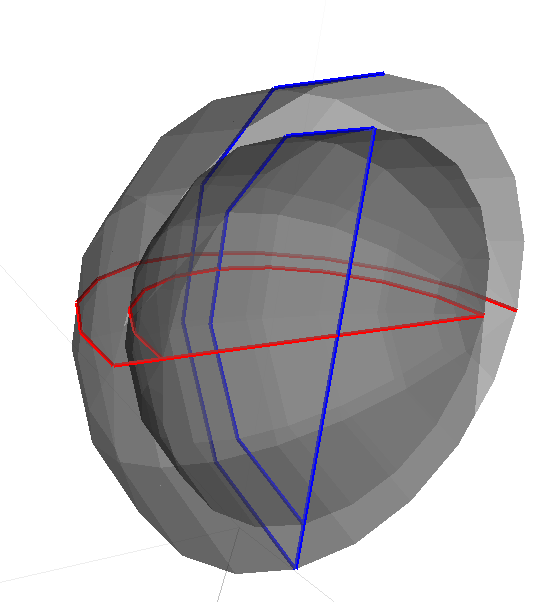
\includegraphics[height=0.5\linewidth]{Images//Booleans/SphereUnion.png}
  \captionof{figure}{Example screenshot of\\ a Boolean Union produced in\\ Pyg4ometry \& viewed in VTK.}
  \label{uni}
\end{minipage}%
\begin{minipage}{.4\textwidth}
  \centering
  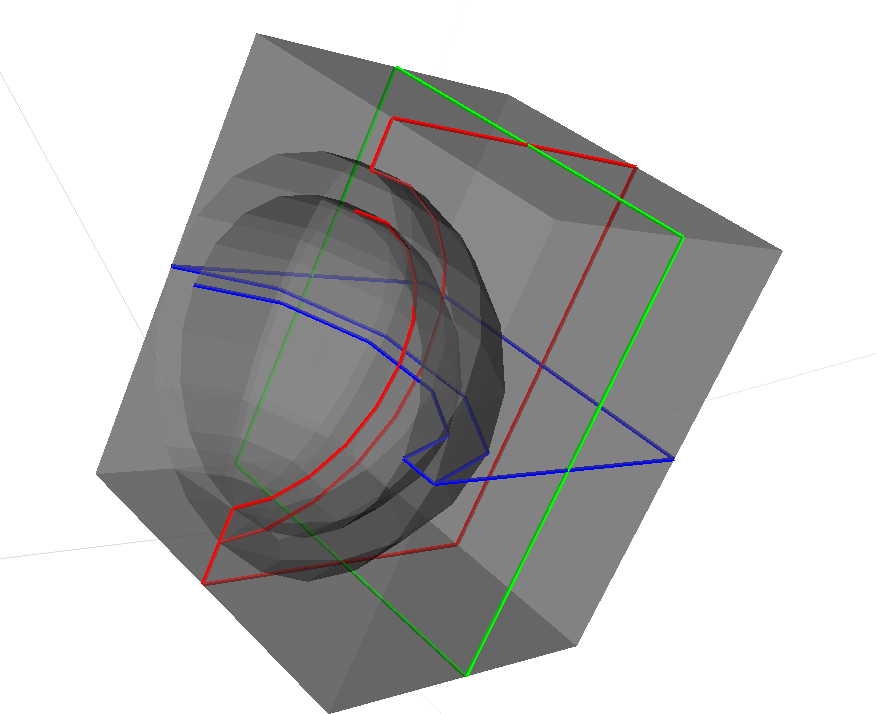
\includegraphics[height=0.5\linewidth]{Images//Booleans//SphereSubtraction.png}
  \captionof{figure}{Example screenshot of \\ a Boolean Subtraction produced\\ in Pyg4ometry \& viewed in VTK.}
  \label{sub}
\end{minipage}%
\end{figure}

\noindent The old meshing algorithms heavily relied on these operations, using intersections to slice solids and subtractions to make solids hollow or cut-up. For example CutTubs (tube with angled ends), as seen in Figure \ref{ct}, can be made from two cylinders and a rotated Box, first the two cylinders would be subtracted from one another, creating regular Tubs (tube), as seen in Appendix Figure \ref{ctub}, then the hollowed out cylinder would be intersected with the the rotated box to create angled tips. In the source code the intersection with a box is actually subtractions with rotated planes, as it is the same concept but more efficient. This basic method has now entirely been replaced with clean trigonometry for all the curved solid meshing scripts in Pyg4ometry.
\\\\
The appearance of the mesh structure itself is also affected by the use of boolean operations, as the boolean operations work by trying to identify common mesh points on the two separate solids, to then remesh between. This created a lot of non-axially uniform mesh sections as seen in solids such as the Hyperboloid, mentioned before in Figure \ref{polypic1}. It can be seen that the new meshing algorithm outputs clean radial faces at for the top and bottom sides of the solid.

\subsubsection{Summary}
As proven by the above examples the boolean operations work and are a much faster way to write the computation of a primitive solid. However this convenience comes at the expense that the boolean operations are very computationally heavy compared with that of the adapted trigonometry which is now implemented in the new method. This is the case especially when one or more of the original solids is curved in structure. The new scripts not only reduce the CPU duration time of running but also neaten the overall appearance of the mesh structures.

\subsection{Meshing Performance Testing}\label{per}
The performance of the meshes was originally investigated by looking at wall time against stack and slice, which was then learned to be a less reliable than CPU time as it can be affected by background processes running on a machine at the same time. The use of CPU time was showing a much clearer trend however still had a large degree of fluctuation and error primarily due to the choice of material, which is explained in more detail when it is employed for other purposes (Section \ref{err}). Therefore it was decided that counting the number of faces created on a given solid was the best measure of the meshes' complexity.

\subsubsection{Polygon Count}
The meshing performance of the Pyg4ometry primitive solids was tested by counting the number of polygons produced by both the old and new meshing algorithms, i.e counting the number of triangular and quadrangular faces on a solid, in order to make a comparison. A plot for each curved primitive solid counting its number of generated polygons was produced, two examples of which can be seen in Figures \ref{conts} \& \ref{hypeup}, and the remaining can be found the Appendix \ref{app1}.
\\\\
They were generated by varying the user input for the number of slices across a range. Most of the solids were put through the range between 10 and 100 slices, whilst keeping the number of stacks at a constant 10. However a few of old meshing scripts took too long to execute at higher mesh densities, leading to a few solids only being measured across a shorter range of slices e.g the old Hyperboloid pycsgmesh function was left to run for a duration of over 2 hours and only collected data up to a slice of 50, as shown in Figure \ref{hypeup}.  \\

\begin{figure}[h!]
\centering
\begin{minipage}{.5\textwidth}
  \centering
  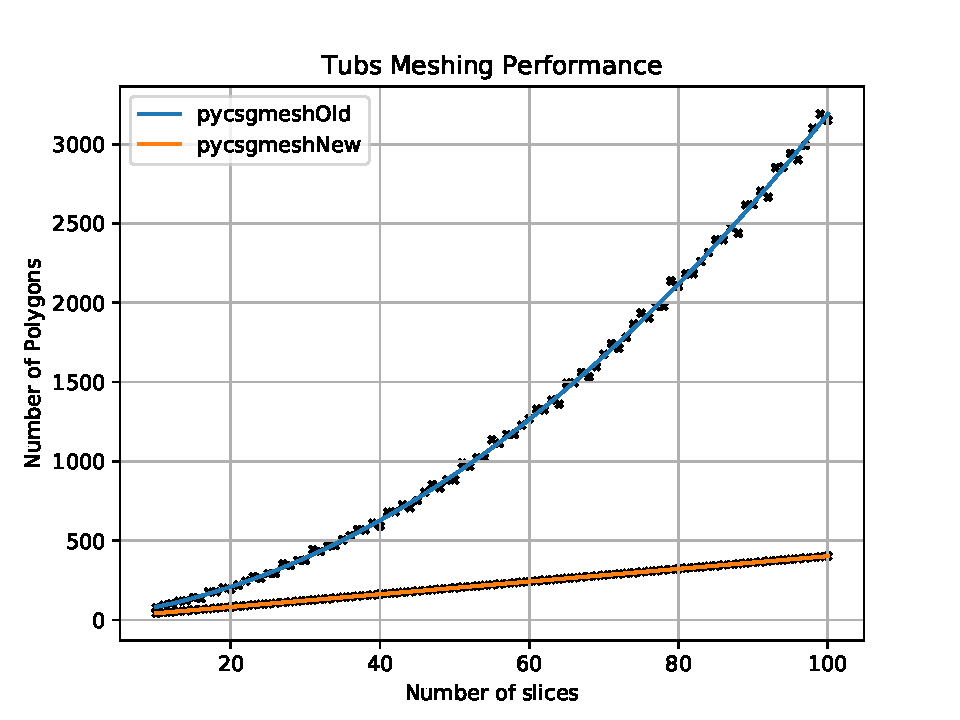
\includegraphics[scale=0.5]{Images//Quad_fits//Tubs_quad.pdf}
  \captionof{figure}{Comparison of the number of\\ polygons (and triangles) generated by the new\\ and old meshing methods, across a range of\\ slices 10-100.}
  \label{conts}
\end{minipage}%
\begin{minipage}{.5\textwidth}
  \centering
  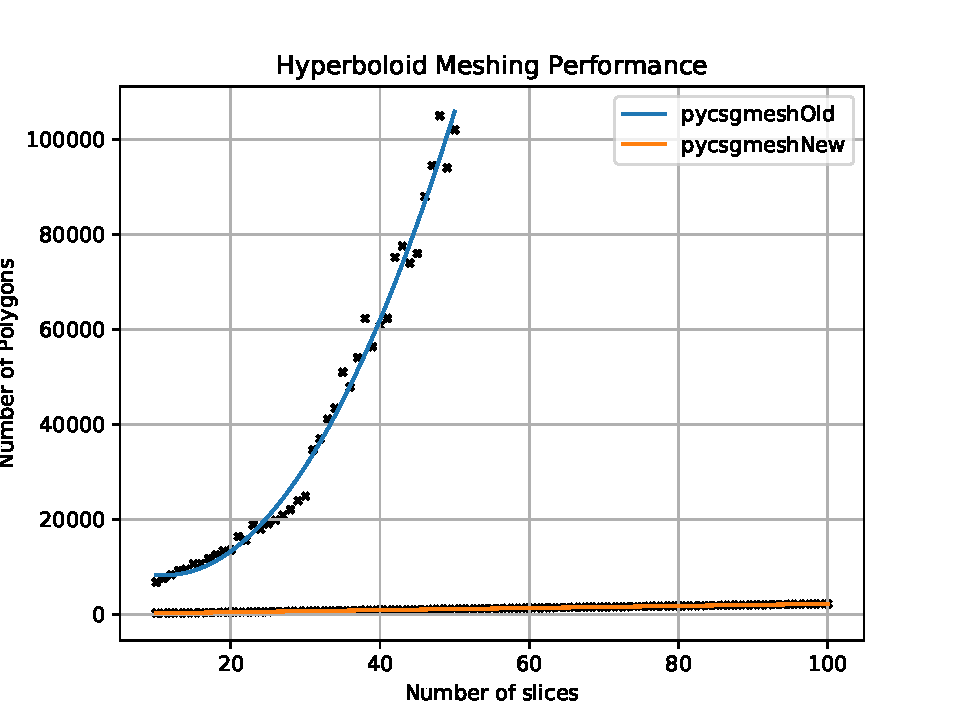
\includegraphics[scale=0.5]{Images//Quad_fits//Hyperboloid_quad.pdf}
  \captionof{figure}{Comparison of the number of\\ polygons (and triangles) generated by the new\\ and old meshing methods, across a range of\\ slices 10-100.}
  \label{hypeup}
\end{minipage}%
\end{figure}

\newpage
\noindent As is clear in both Figures, the new meshing function is less computationally expensive compared with the old meshing functions, generating far fewer faces per slice and stack. The number of polygons increases more uniformly and linearly for the new pycsgmesh function. The old pycsgmesh function exhibits a more scattered and quadratic relationship, due to the boolean operations. This is also confirmed by the values tabled in the Appendix \ref{tab1}, which contains the quadratic fitting parameters to all the polygon count plots. If both graphs are extrapolated, it is clear than the new mesh is not only improving the structural appearance of the meshed solids, but also saving large amounts of computational power and time.
\\\label{recur}\\

%---------------------------------------------------------------------------------------------------
%---------------------------------------------------------------------------------------------------
%---------------------------------------------------------------------------------------------------

\section{BDSIM Geometry Simulation}
\label{int}
The second aim of this project was to measure how the physics is altered between the new and old meshings as the mesh density is varied. As mentioned before GEANT4 already has its own set of primitive solids, which can be used as a guideline for comparison, due to no slice and stack dependence. The physics being measured will be features such as the trajectories and energy deposition, through solids.

\begin{figure}[h!]
\centering
\includegraphics[scale=0.33]{Images//BDSIM//titanium.pdf}
\caption[width=\columnwidth]{A BDSIM screenshot of a G4\_W Pyg4ometry Sphere generated with new meshing interacting with 100 1.3 GeV electrons.}
\label{black}
\end{figure}

\noindent Figure\ref{black} shows a spherical distribution of 100 1.3 GeV electrons radiating outwards from the centre of a Pyg4ometry G4\_Ti Sphere, where negatively charged red tracks and neutral green tracks can be seen, which are most likely electrons and photons. A secondary particle is anything that is produced as a result of the initial particles interacting with the solid, therefore a secondary itself can produce another particle which is considered to also be  a secondary particle. The Monte Carlo simulation in BDSIM uses a numbering system for identifying particles, assigning each particle a unique number. The numbering system adopted in BDSIM is the one used by GEANT4 and created by PDG (or the Particle Data Group) \cite{pdg}, which is an international collaboration dedicated to analysing and publishing the properties of particles. 

\subsection{Monte Carlo Simulation}
\label{monte}
\noindent The probability of certain particle interactions occurring in a given BDSIM event, such as the decays or scattering of a particles trajectories is generated by a Monte Carlo simulation. The basic principle behind the Monte Carlo algorithms is the use of large random sampling to find numerical results. This is perfect for simulating the probabilities of particular particle interactions happening, as two initially identical interaction setups can have two non-identical interactions, with a given probability. Each event in BDSIM is associated with a specific seed number produced via this Monte Carlo method. The uniqueness of each seed allows a particular event to be repeatedly simulated under the same physics conditions, which is key to this project when it comes to comparing the interactions of different objects fairly. The other properties of the particle and physics processes that may occur can also be user defined to tweak the experiment. Properties such as the particles initial energy, whether secondaries get produced and much more. The seeds used in this project could not be logically chosen due to the fact they are generated via the Monte Carlo simulation. Therefore they were selected by running a lot of test runs in BDSIM to see which seeds generate an adequate amount of secondaries.

\subsection{Simple Solid Target}
The meshed solid chosen to be tested within BDSIM for this project was the Sphere, which is made of a minimum and maximum radius, making it a hollow solid. The reason a Sphere was chosen because it is the ideal shape testing radiation in all directions, as its thickness can be controlled radially. As seen in Figure \ref{sphbd} the Sphere was orginally chosen to be oriented such that the particle beam is fired from the centre of the Sphere outwards. The conversion from a Pyg4ometry mesh into a GEANT4 tessellated solid, results in only triangular faces. This is why all the quadrilateral faces are cut into two in Figures \ref{black} \& \ref{sphbd}.

\begin{figure}[h!]
\centering
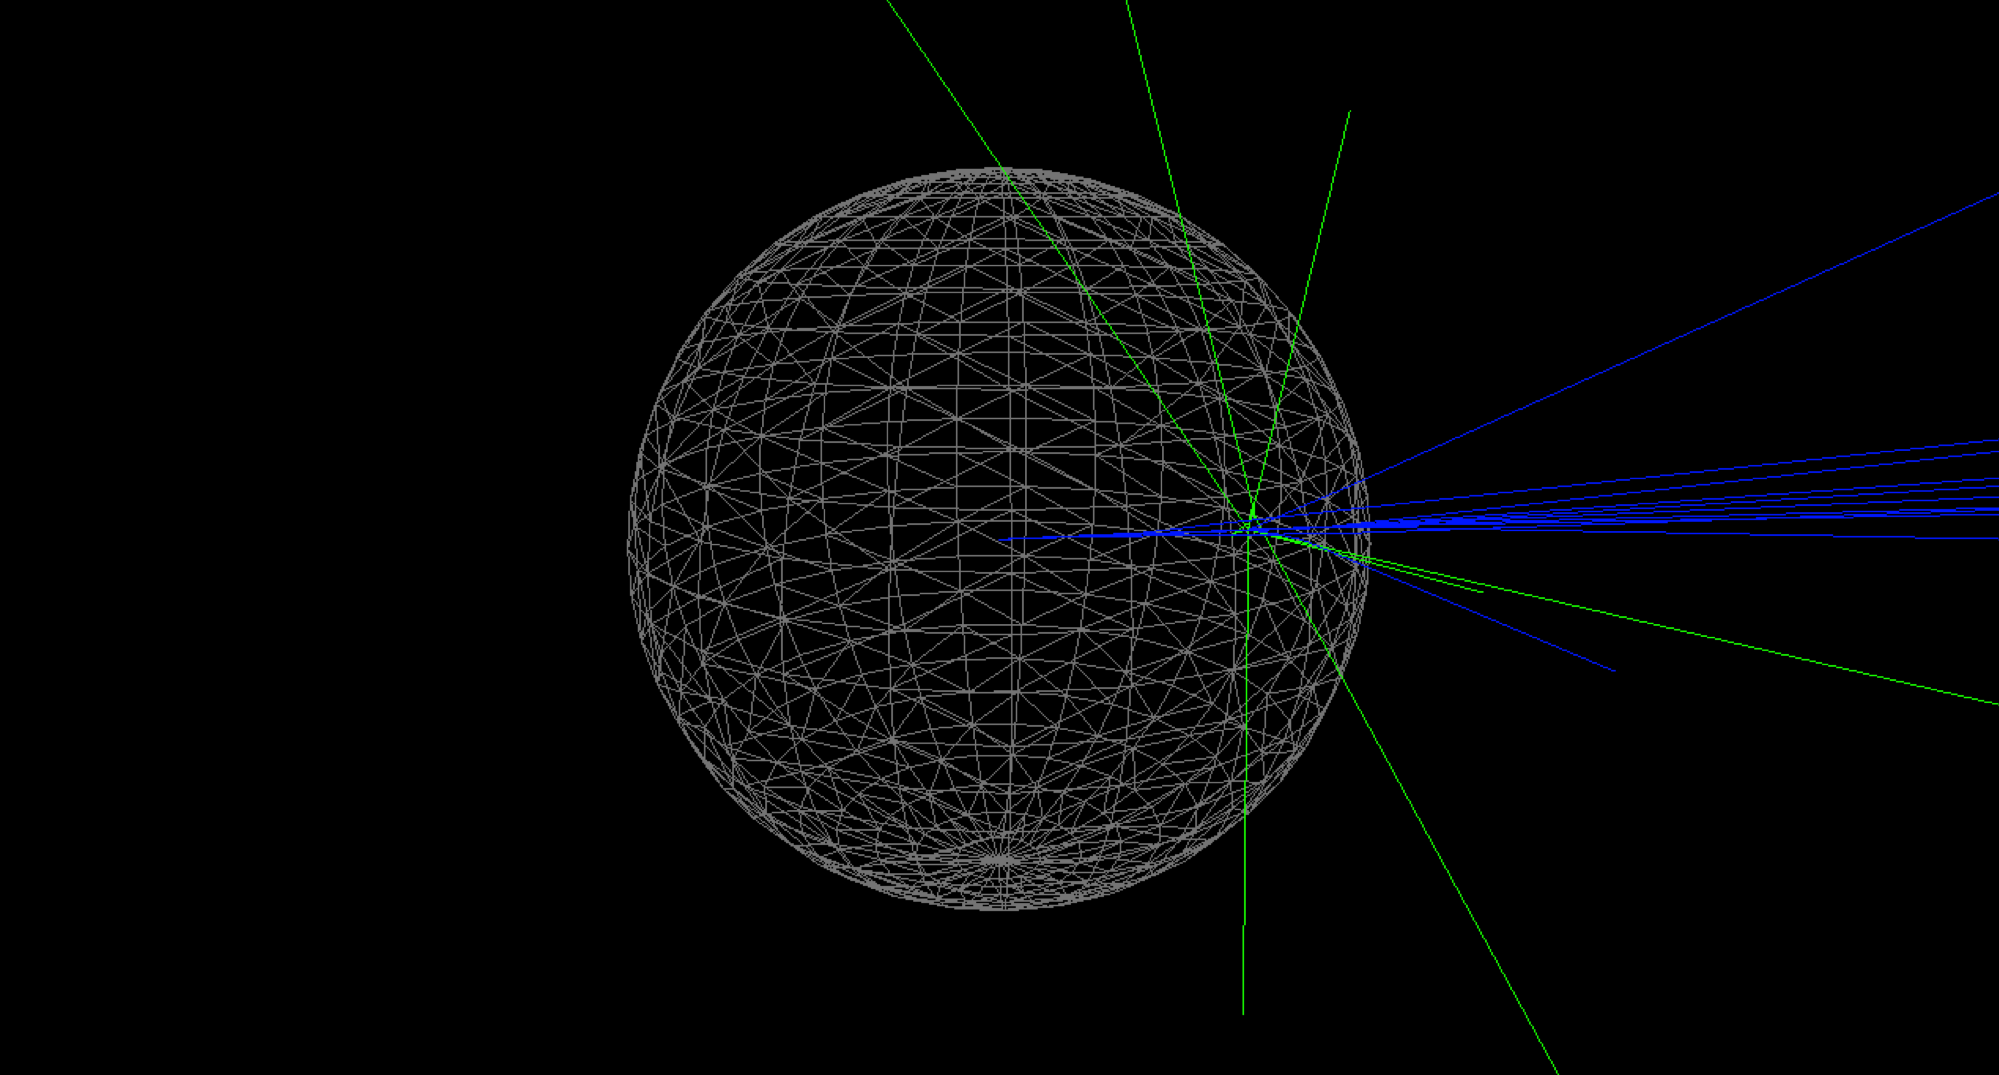
\includegraphics[scale=0.35]{Images//BDSIM//ProtonSphere2.png}
\caption[width=\columnwidth]{BDSIM screenshot of 10 1.3 GeV protons interacting with a G4\_Fe Sphere, which has been constructed using the new Pyg4ometry meshing scripts. Mesh resolution is a stack of 25 and slice of 25. (Shown in mesh view)}
\label{sphbd}
\end{figure}

\subsection{Titanium Sphere Interactions}
This section investigates the CPU duration time of simulated particle interactions in BDSIM, comparing Spheres that are constructed by different meshing algorithms as a way to analyse the energy deposition as the mesh density is increased. Table \ref{tab11} shows the properties of the Spheres being meshed and the simulation setup, ``ngenerate'' is a BDSIM parameter to specify the number of particles in a given run. In this scenario the preset GEANT4 Sphere was used as a guideline as it does not depend on a user defined stack \& slice. 
 
\begin{table}[h!]
\centering
\begin{tabular}{|l|l|}
\hline
Property & Value \\ \hline
$R_{Min}$ &  10.00 [\mu m]\\ \hline
$R_{Max}$ &  10.00 [mm]\\ \hline
Particle &  $e^-$\\ \hline
Energy & 1.3 GeV [MeV]\\ \hline
ngenerate & 10,000\\ \hline
\end{tabular}
\caption{Table of simulation properties for the simulations in this section.}
\label{tab11}
\end{table}
\noindent To begin with all the GDML Spheres were created, this was first in the aim of being more productive, as the creating the GDML targets typically takes longer than to execute an interaction in BDSIM. Therefore once the GDMLs are all correctly made, the time taken for simulations and plots is largely reduced. Also by outputting the data after each run, this increases the ease of adjusting plots. The same analysis performed in Section \ref{per} was applied to the created GDMLS and can be seen in Figure \ref{tritri}.

\begin{figure}[h!]
\centering
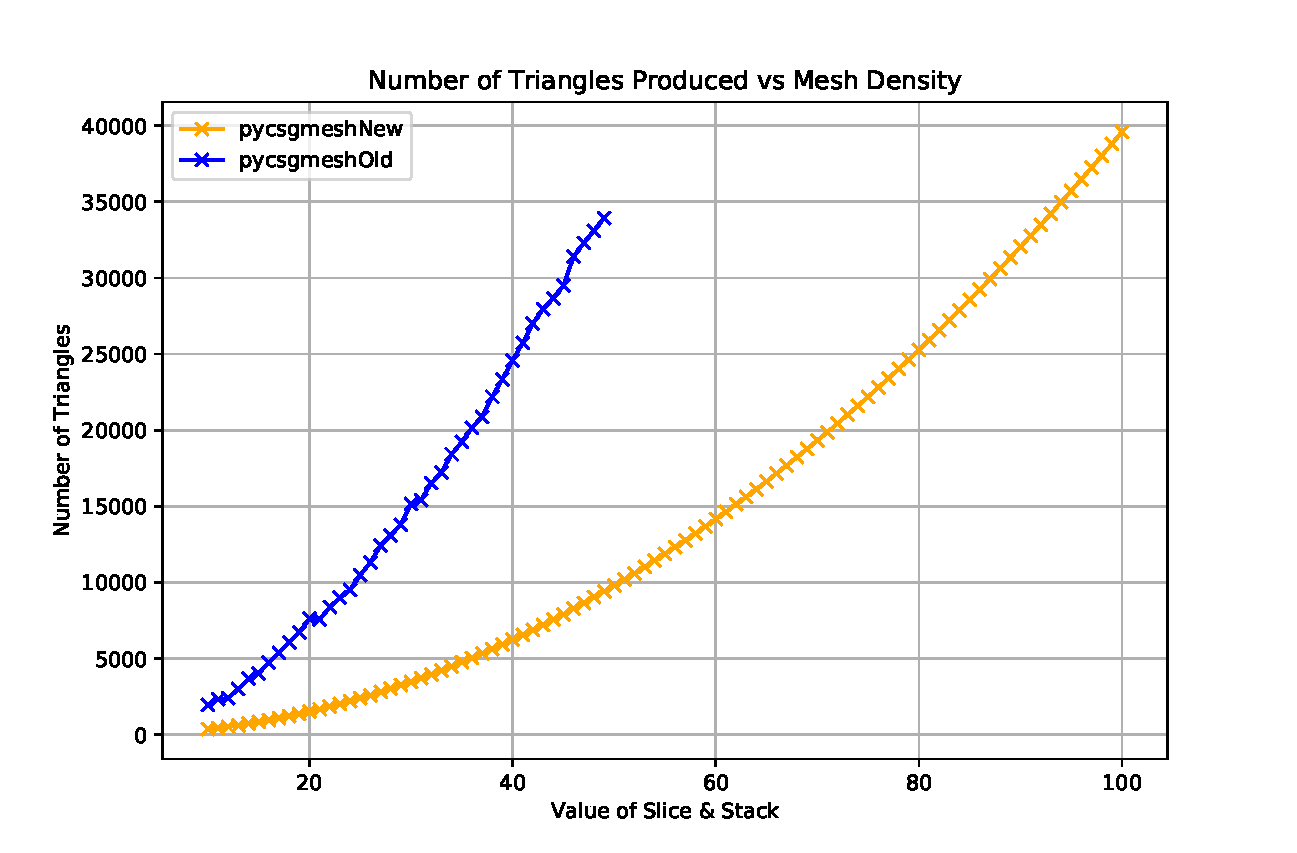
\includegraphics[height=.4\linewidth]{Images//Triangles//MeshvTRi1.pdf}
\caption[width=\columnwidth]{A plot showing the stack and slice against the number of polygonal faces produced on a Sphere with the set dimensions for the proceeding section, shown for both meshing algorithms new (orange) and old (blue).}
\label{tritri}
\end{figure}
\noindent The Figure \ref{tritri} shows the total number of triangles on the interior and exterior surfaces for a given slice and stack equal to the same value on a G4\_Ti Sphere. The old meshing algorithm only meshed up to a maximum resolution of slice and stack equaling 48, before it would max out Python's recursion limit, whereas the new meshing could go to stack of 100 and a slice of 100 without any issues at all. The recursion limit can be extended to allow for a larger range, however it would not be worth the time it would take to code and run. 
It can be seen that in Figure \ref{tritri} the new pycsgmesh function has a much smoother gradient and that the old function has small peaks occurring at certain intervals of stack and slice. This is most likely to do with the boolean subtractions of the Spheres favouring the old mesh at particular densities. To avoid confusion with the polygon count plot for the Sphere in the Appendix (Figure \ref{aphh}) it should be made clear that the two plots are testing two differently meshed Spheres across different variations of slice and stack. The one in the appendix is an incomplete Sphere missing wedges in both its slice and stack, compared with the one tested in Figure \ref{tritri}, which is a complete Sphere tessellated purely out of triangles.  This plot confirms the GDML are all in the expected format, to begin interaction.
 \\\\
\noindent The interactions were automated using Pybdsim within a specially written Python script. The script worked by creating a GMAD file from a template, which would then specify which GDML Sphere it was placing into the simulation environment, and then using Pybdsim to execute the simulation and extract data from the outputted ROOT files. The Python script ran this processes in a ``for loop'' iterating through each GDML target and appending its data to an external TXT file, the results of which can be seen in Figure \ref{withs}.

\begin{figure}[h!]
\centering
\begin{minipage}{.5\textwidth}
  \centering
  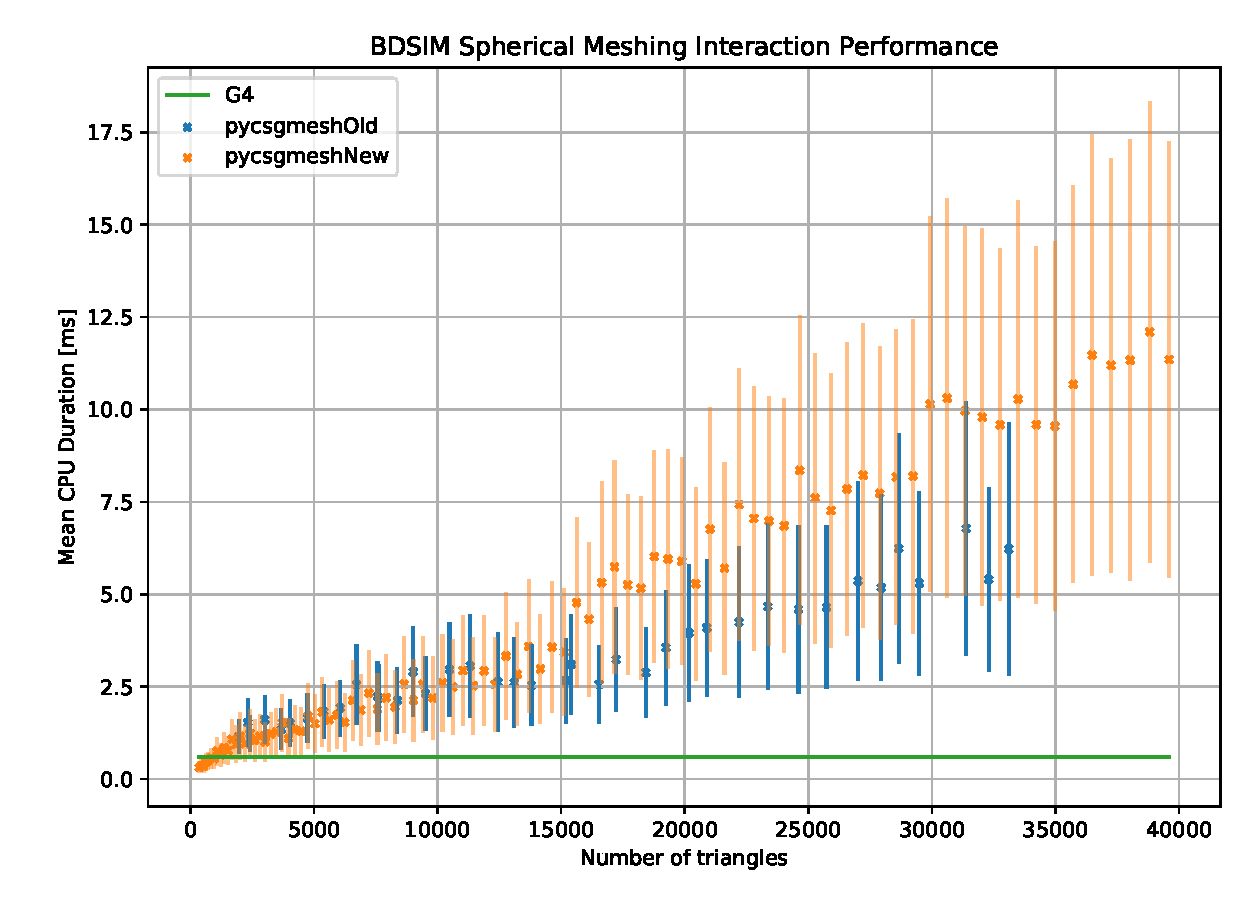
\includegraphics[height=0.7\linewidth]{Images//CPU//Total_Plot_with_secondaries.pdf}
  \captionof{figure}{Mean CPU duration of 10,000\\ protons interacting with a G4\_Ti Sphere of \\various meshed forms.\\}
  \label{withs}
\end{minipage}%
\begin{minipage}{.5\textwidth}
  \centering
  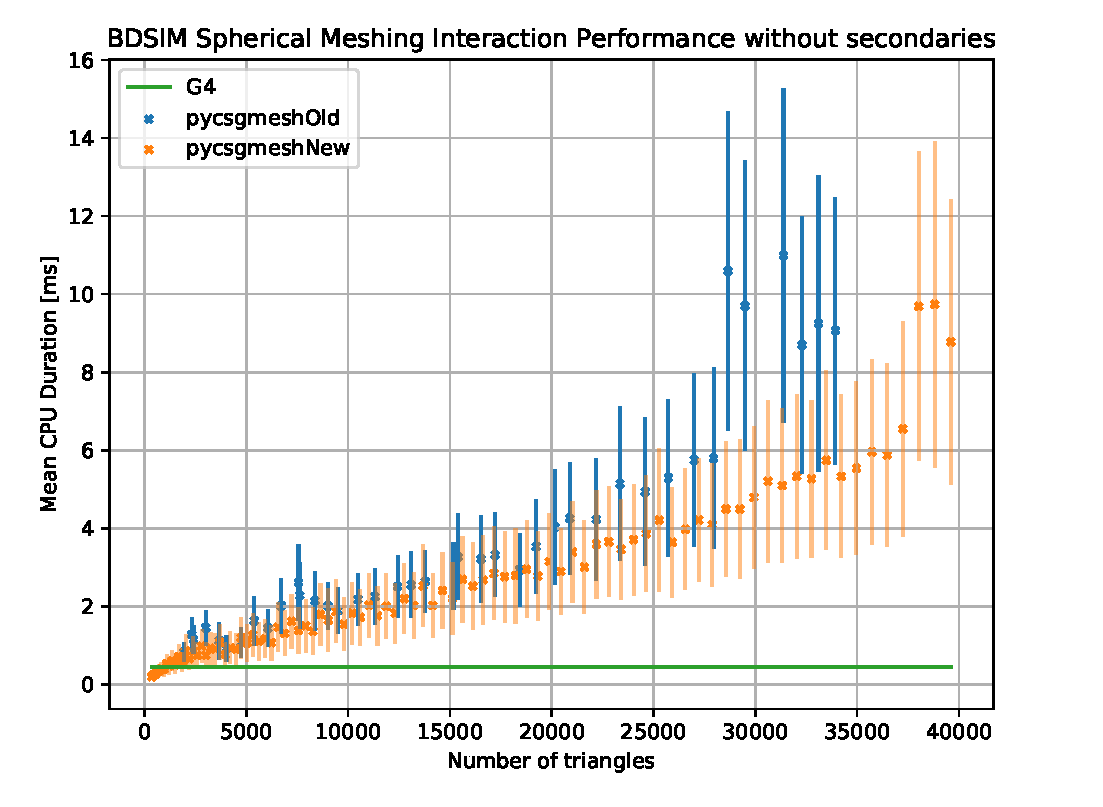
\includegraphics[height=0.7\linewidth]{{Images//CPU//Total_Plot_no_secondaries1.pdf}}
  \captionof{figure}{Mean CPU duration of 10,000\\ protons interacting with a G4\_Ti Sphere of \\various meshed forms, with secondary\\ particles disabled.}
  \label{withouts}
\end{minipage}%
\end{figure}

\noindent Figure \ref{withs} shows the mean CPU duration times for an interaction in BDSIM with a given Sphere. The x-axis was originally the number of stack and slice, but it was thought that the number of triangular faces created on a given Sphere would give a fairer weighting between meshing algorithms. This is due to the fact the number of faces increases at different rates dependent of the meshing algorithm used, as shown earlier by Figure \ref{tritri}. The reason there is nearly twice as many points plotted for the new meshing over the old is because of the recursion limit, which is discussed in Section \ref{recur}. The error bars in Figure \ref{withs} are the standard deviation of each run; the material of the Sphere was originally chosen to be G4\_Fe which is much less dense and caused many more secondaries than G4\_Ti, making the error bars dominate the data trend. The change of material from G4\_Fe to G4\_Ti was chosen as G4\_Ti is not only much denser but also has a larger stopping power (Section \ref{stop}). Figure \ref{withouts} is the same simulation as in Figure \ref{withs}, but has secondary particles disabled. The reason for Figure \ref{withouts} was to investigate whether the number of secondaries produced has an effect on the duration of the interaction. As it can be seen the number of secondaries produced partially relates to the size of the standard deviation, but not by a very large margin.

\newpage
\subsubsection{Error Reduction}
\label{err}
\noindent In attempt to further reduce the standard deviation of a data set the number of events was increased, the theory behind this came from the relationship shown by %in Equation \ref{a}. The equations show that the standard deviation is inversely proportional to the square root of the number of events. Therefore in theory the standard deviation should decrease with increasing N.

\begin{equation}
\begin{aligned}
& \bar{x} = \frac{1}{N}\sum{x_i}\\
& \sigma = \sqrt{\bar{x}^2} = \sqrt{\frac{1}{N}\sum{(x_i - \bar{x}})^2}\\
& \sigma \propto \frac{1}{\sqrt{N}} .
\end{aligned}
\label{a}
\end{equation}

The equations show that the standard deviation is inversely proportional to the square root of the number of events. Therefore in theory the standard deviation should decrease with increasing N, however, the error bars did not fluctuate in size to the degree that was expected despite the number of events being increased. This is shown by Figure \ref{err}, which is a plot made with a G4\_Fe Sphere before the switch to G4\_Ti was made, but the purpose of the plot still holds. 

\begin{figure}[h!]
\centering
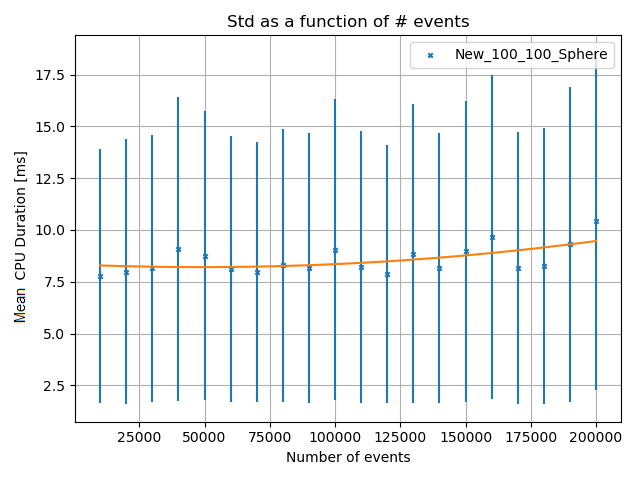
\includegraphics[scale=0.6]{Images//Error//std_N1.png}
\caption[width=\columnwidth]{Mean and standard deviation of the CPU duration distribution of an interaction as the number of initial particles is increased. The interaction modeled was 1.3 GeV electrons against newly meshed G4\_Fe Sphere with a stack of 100 and slice of 100.}
\label{err}
\end{figure}

\noindent It was then concluded that the number of particles being ran in each event was already sufficiently high that one would not see much fluctuation in the size of the standard deviation no matter how many more particles were fired. The real reason for the standard deviations being so large is that there is a small number of particles within each simulation run, where a large number of secondaries are being produced, resulting in a longer overall event duration and in turn lengthens the standard deviation. An example of this is shown in Figure \ref{disty}, where the plot shows the CPU distribution for 10,000 10 MeV electrons interacting with a G4\_Ti Sphere. The Sphere in this example is constructed using the new pycsgmesh function with a stack and slice both set at 100.

\begin{figure}[h!]
\centering
\includegraphics[scale=0.5]{Images//CPU//Pythonhist1.pdf}
\caption[width=\columnwidth]{A  histogram showing a CPU duration distribution for 10,000 1.3 GeV electrons intersecting with a Sphere that has been meshed using the new pycsgmesh function. The density of the mesh was set to slice and stack both equal to 100.}
\label{disty}
\end{figure}

\noindent This was then backed up by replotting the original simulation, but plotting the median and maximum values with increasing number of triangular faces, which is shown in Figure \ref{mednmax}, in which one can see most of the fluctuation in the data is in the maximum values of the distributions. This complements the theory of a few particles causing large skews in the overall standard deviations.

\begin{figure}[h!]
\centering
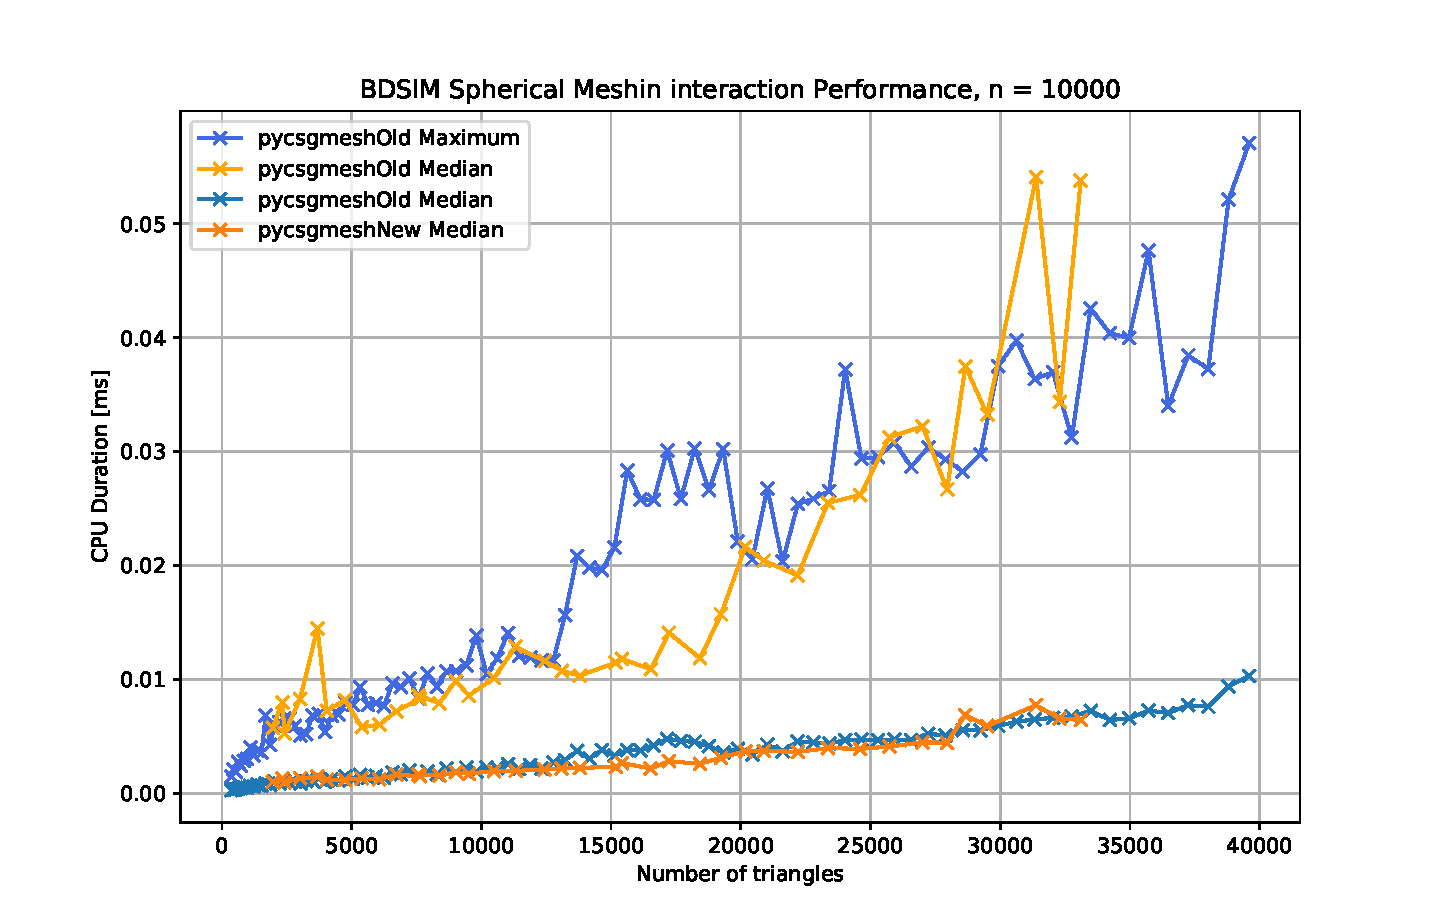
\includegraphics[scale=0.6]{Images//CPU//mednmax.pdf}
\caption[width=\columnwidth]{The number of polygonal faces in a mesh plotted against the median and maximum values of the CPU duration distribution, displayed for both the new meshing (orange)  and the old meshing (blue).}
\label{mednmax}
\end{figure}


\newpage
\subsection{Selection of Material}
When creating any solid, one has the choice of material. Figure \ref{novar} shows the CPU duration time distributions for electron interactions with preset GEANT4 Spheres constructed of different GEANT4 materials across a range of energies in BDSIM. The energy range is relatively low (25 MeV $\rightarrow$ 100 MeV), this is due to the run time being heavily linked to the number of secondary particles produced as a function of energy. This is proven by the fact that it can be seen that as the energy is increased the width of the distribution increases. This widening is due to the increase in number of secondary particles being produced; the more energetic an interaction the further the particle will penetrate a solid and ionise, along the way generating more secondaries.
\begin{figure}[h!]
\centering
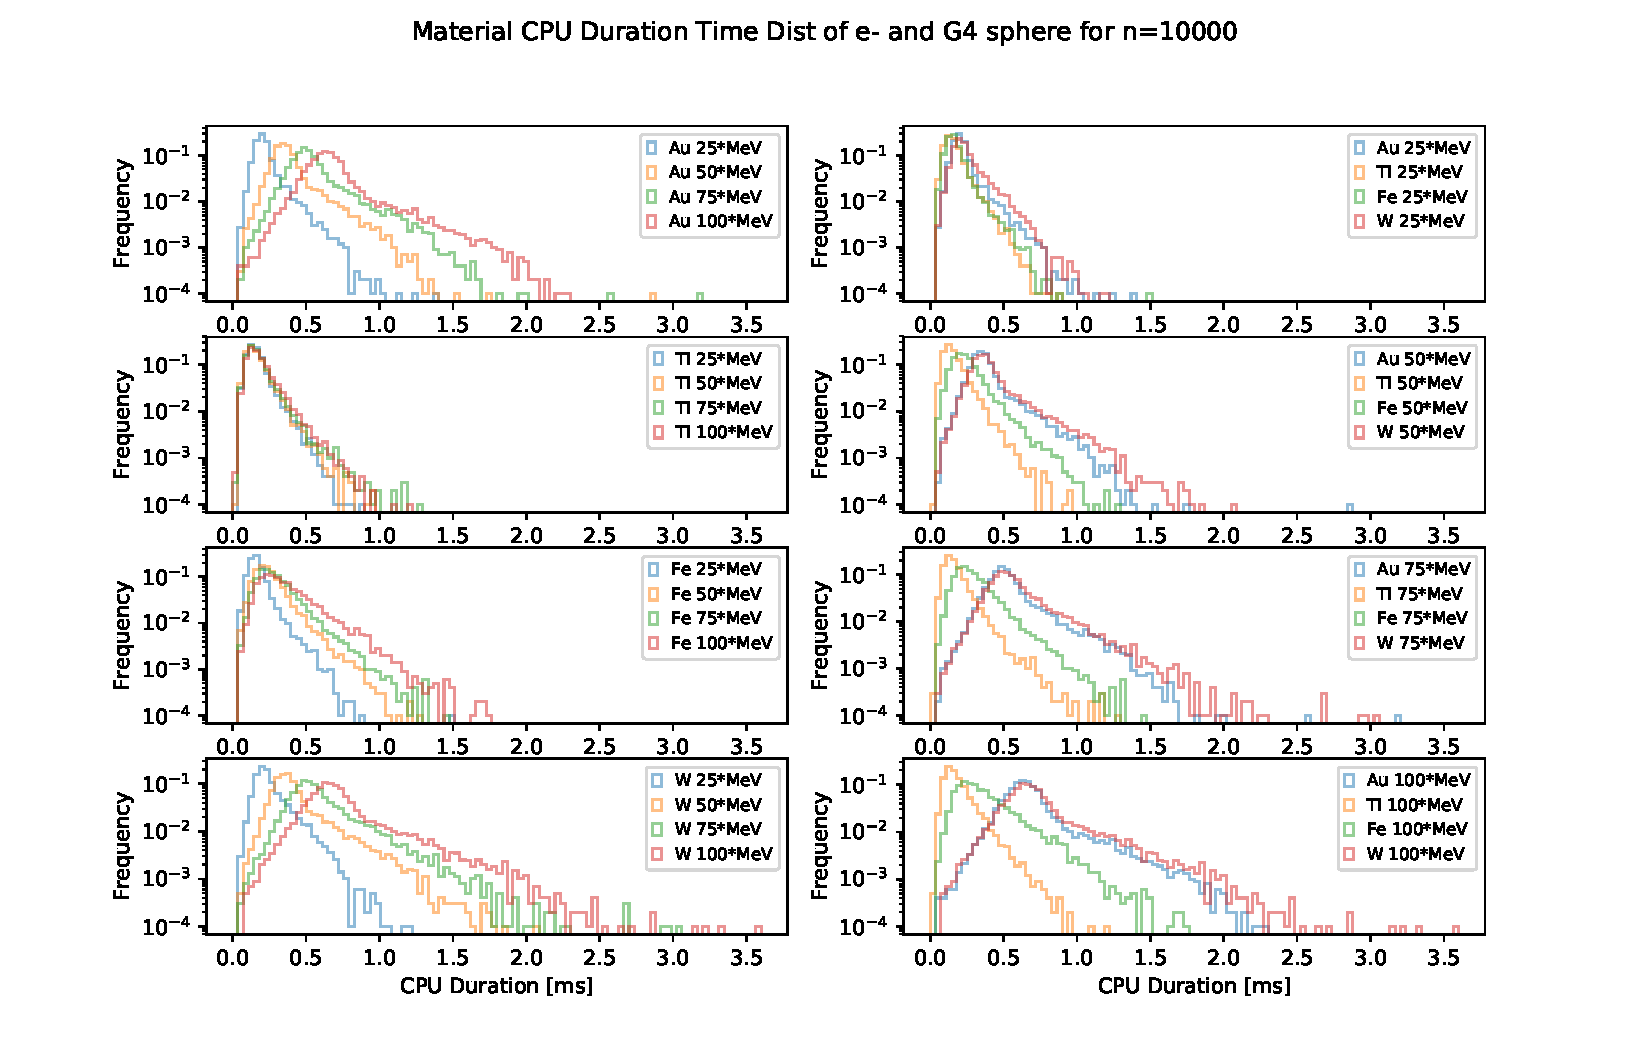
\includegraphics[scale=0.6]{Images//Materials//not_Varied_by_radius_and_secondaries.pdf}
\caption[width=\columnwidth]{Histograms showing the CPU duration distributions of varying GEANT4 materials and particle energies in BDSIM on a GEANT4 Sphere. The left 4 histograms show the distributions show the varying of energy upon each material. The right 4 histograms show the varying of material at each set energy. Each plot is normalised by the initial 10,000 electrons in each event.}
\label{novar}
\end{figure}
\newpage
\noindent The dimensions of the Spheres used in Figure \ref{novar} were set to a minimum radius of 1 micron and a maximum radius of 10 mm. It was then proposed that the radius of thickness could be scaled with respect to the stopping distance of the material it is travelling through, in order to eliminate material as a variable. The radius of thickness $\Delta R$ can be seen depicted in Figure \ref{deltar}, where $\Delta R = R_{Max} - R_{Min}$.

\begin{figure}[h!]
\centering
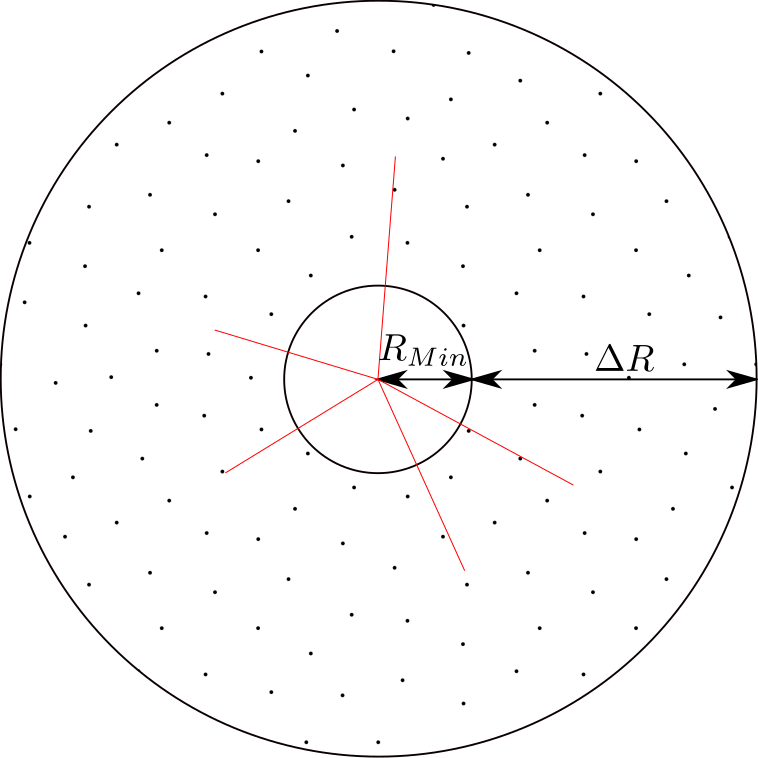
\includegraphics[scale=0.2]{Images//Materials//RMAX.png}
\caption[width=\columnwidth]{A diagram depicting a cross-section of a Sphere, which has a minimum and maximum radius.}
\label{deltar}
\end{figure}

\newpage
\subsubsection{Stopping Power}
\label{stop}
Stopping power is the force that acts against the motion of a particle within in a material, causing it to lose energy. A charged particle is mainly slowed down by electronic stopping as it moves along a linear trajectory. Electronic stopping is the inelastic energy loss to the electrons of the target as a result of thermal vibrations at an atomic level. The electronic stopping contributes most in the intermediate energy range of a travelling particle, as seen in Figure \ref{stprg}. Once the particle has lost a sufficient amount of its energy, slowing its velocity through the target, the probability of an elastic collision with a nuclei increases (Nuclear Stopping). The nuclear stopping is the process which causes damage to the target, as the target atom recoils way after the interaction causing a disorder in the lattice structure of the target. The recoiled atom can also go on to cause further collisions causing yet more damage. As seen in Figure \ref{stprg} the electronic stopping power dominates and the nuclear stopping only needs to be accounted for at very low energies.
\\\\
\begin{figure}[h!]
\centering
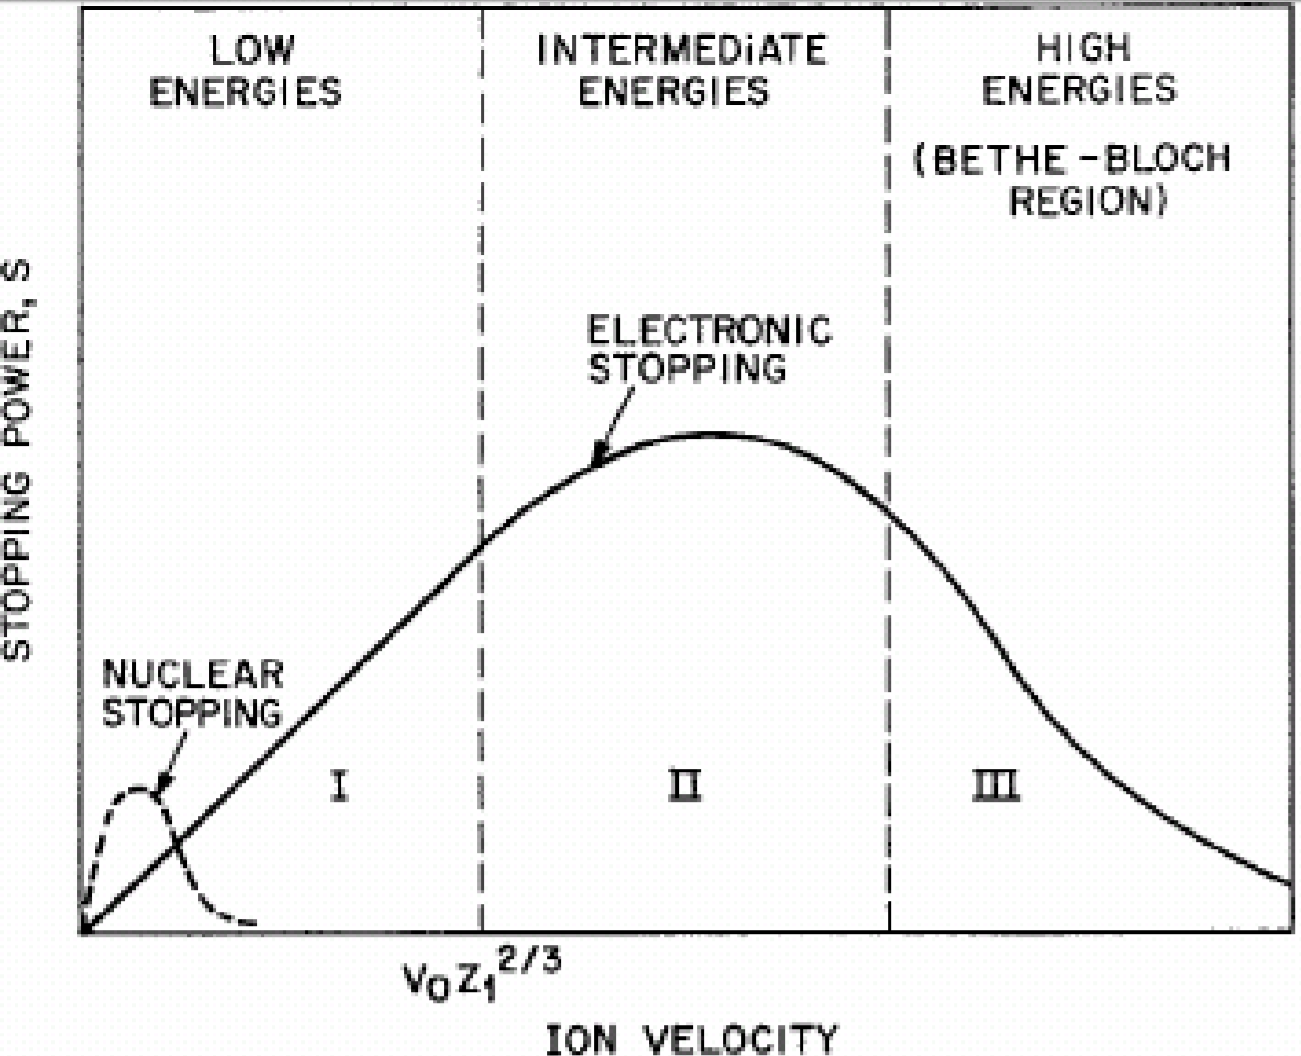
\includegraphics[scale=0.4]{Images//Stopping//stoppingrange.png}
\caption[width=\columnwidth]{The relationship between ion velocity and components of stopping power, from Source \cite{stprg}}
\label{stprg}
\end{figure}
\\\\
\noindent GEANT4 comes with some supplementary examples, the example ``TestEm0'' \cite{emo} outputs the stopping power and distances for a given material and particle energy. If the energy of the incident particle and the stopping power of the material is known, a stopping distance can be calculated. The values for stopping power in this project are calculated by the TestEm0 example, which extracting values from a GEANT4 data lists and then interpolates or extrapolates between them, as the stopping power is a function of energy. The extracted stopping powers match with values found in other studies, such as \cite{stpdat}.
\\\\
\noindent With the stopping power in mind Figure \ref{novar} was reproduced, but instead of using the same dimensions for each Sphere, $\Delta R$ was scaled by the stopping distance of the material. The radius of thickness is set to be the extracted stopping distance for a 100 MeV electron interacting with the material in question. The values of $\Delta R$ are shown in Table \ref{rs}.
\newpage
\begin{table}[h!]
\centering
\begin{tabular}{|l|l|}
\hline
Material & $\Delta R$ [mm] \\ \hline
G4\_Au &  9.89382\\ \hline
G4\_Ti &  33.6854\\ \hline
G4\_Fe &  62.3434\\ \hline
G4\_W &  10.1631\\ \hline
\end{tabular}
\caption{A table showing the values of $\Delta R$ used in Figure \ref{var}.}
\label{rs}
\end{table}
\noindent It can be seen that in Figure \ref{var}, the scaling of radius relative to stopping distances, generates histograms which act in an extremely similar fashion at the same particle energies irrespective of the material it propagates through. This is very interesting as it means that for any further analysis, material can be ruled out as a variable and only energy needs to be varied.
\\\\
\begin{figure}[h!]
\centering
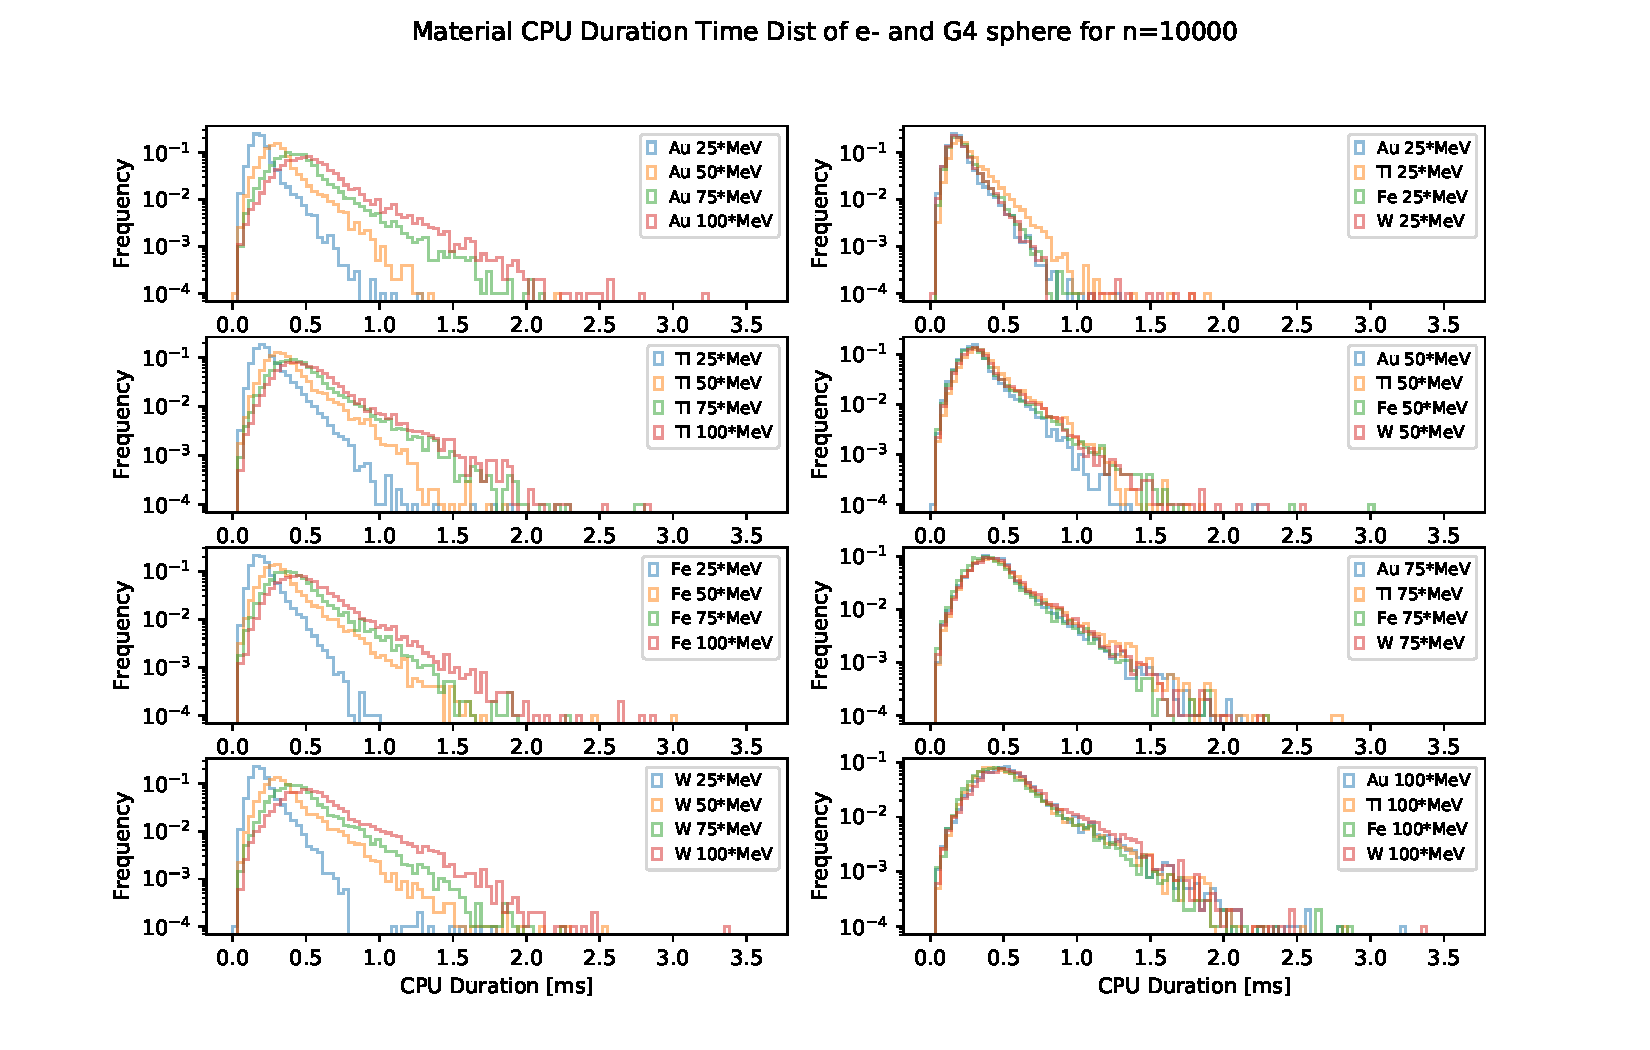
\includegraphics[scale=0.6]{Images//Materials//Varied_by_radius_and_secondaries.pdf}
\caption[width=\columnwidth]{Histograms showing the CPU duration distributions of varying materials and particle energies in BDSIM on a GEANT4 Sphere. The left 4 histograms show the distributions show the varying of energy on each material. The right 4 histograms show the varying of material at a set energy. Each plot is normalised by the initial 10,000 electrons in each event.}
\label{var}
\end{figure}
\\
\noindent The effect is visualised by Figure \ref{tung}, which shows a Sphere made of G4\_W, undergoing interactions with batches of 100 electrons at 3 different energies. The radial thickness ($\Delta R$) of all three Spheres is set to the be the stopping distance for G4\_W interacting with a 1 TeV electron. It can be seen that when the energy of the electrons is 1 GeV, which is below the 1 TeV threshold, the tracks of the interactions are all contained within the Sphere. The opposite happens when the electrons energies are more than 1 TeV, where most if not all of the particle tracks leave the Sphere. However, when the energy of the electron travels through its required stopping distance $\Delta R$, the maximum amount of radiation can be contained within the Sphere with minimum escapes. This concept is what causes all the histograms to become near identical in Figure \ref{novar}, as they are all using their relative stopping distances as a $\Delta R$ scaling.

\begin{figure}[h!]
\hspace*{1.4cm}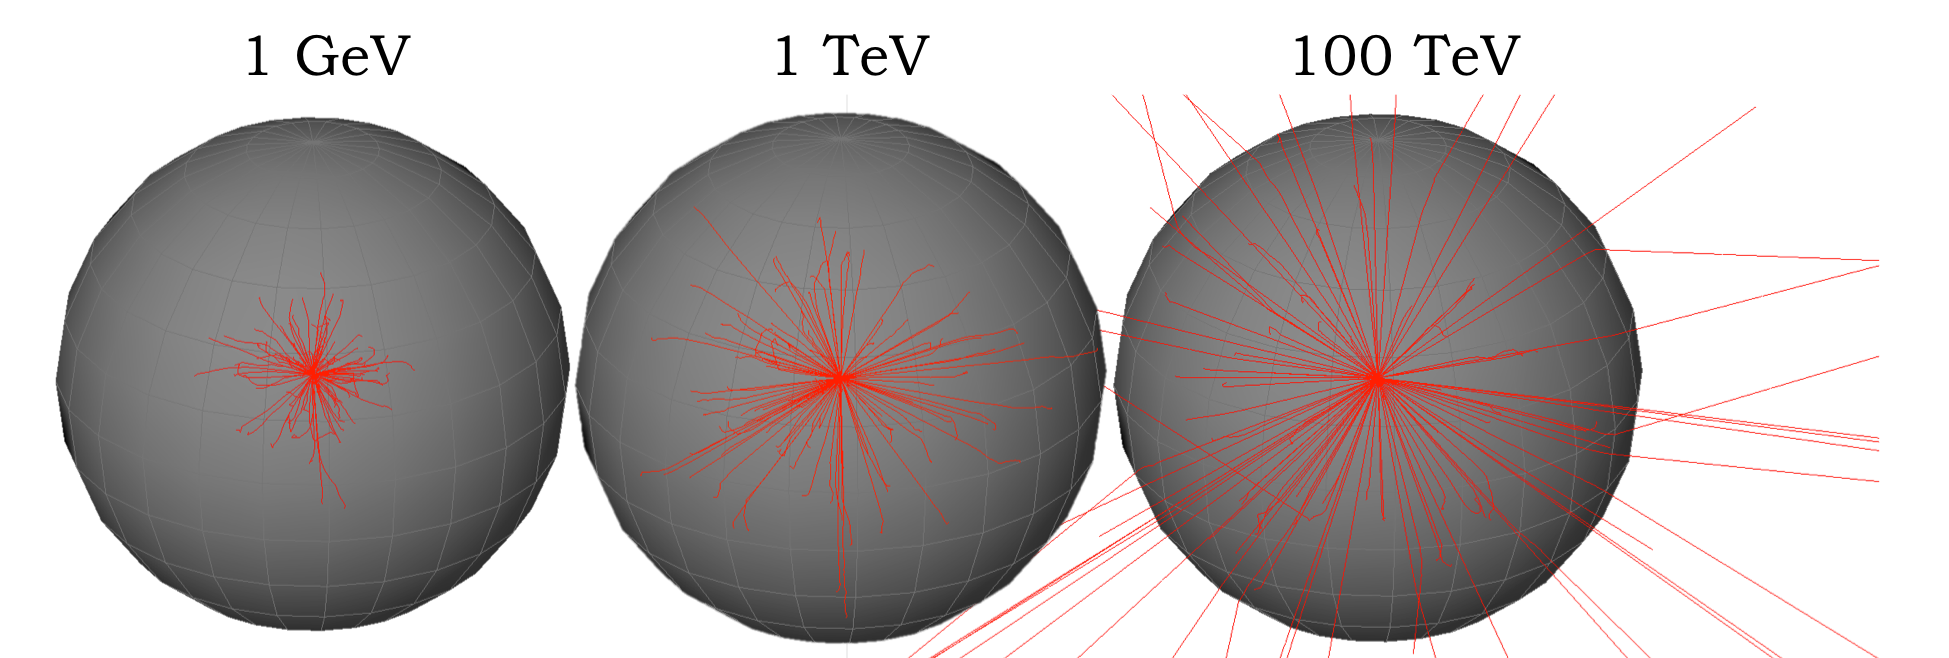
\includegraphics[scale=0.5]{Images//BDSIM//Tungsten_Sphere.png}
\caption[width=\columnwidth]{Screenshots of 1 GeV, 1 TeV \& 100 TeV electrons interacting with a tungsten Sphere. The radius of thickness is set to the extracted GEANT4 stopping distance of a 1 TeV electron in G4\_W.}
\label{tung}
\end{figure}

\subsection{Interactions with CAD}
As a final goal to round off the project, imported CAD models were compared with a compound boolean meshed solids. The first CAD model was of a generic bolt, shown in Figure \ref{notmybolt}. The CAD bolt was downloaded as a STEP format from a free online database GradCAD \cite{cadmag}. The downloaded model was converted to GDML format with the material G4\_STAINLESS-STEEL using Python. The dimensions of the CAD model were gained by using the measuring tool within the FreeCAD GUI as shown Figure \ref{boltinfreeCAD}. The CAD model was then approximately recreated by the construction of basic primitive solids with boolean operations in Pyg4ometry and can be seen in Figure \ref{boltinvtk}.
\\
\begin{figure}[h!]
\centering
\begin{minipage}{.7\textwidth}
  \centering
  \includegraphics[width=1\textwidth]{Images//CAD_Screw//freeCADbolt.png}
  \captionof{figure}{Imported CAD model in FreeCAD, with dimensions \\ via FreeCAD's measuring tool.}
  \label{boltinfreeCAD}
\end{minipage}%
\begin{minipage}{.3\textwidth}
  \centering
  \vspace{5mm}
  \hspace{2cm}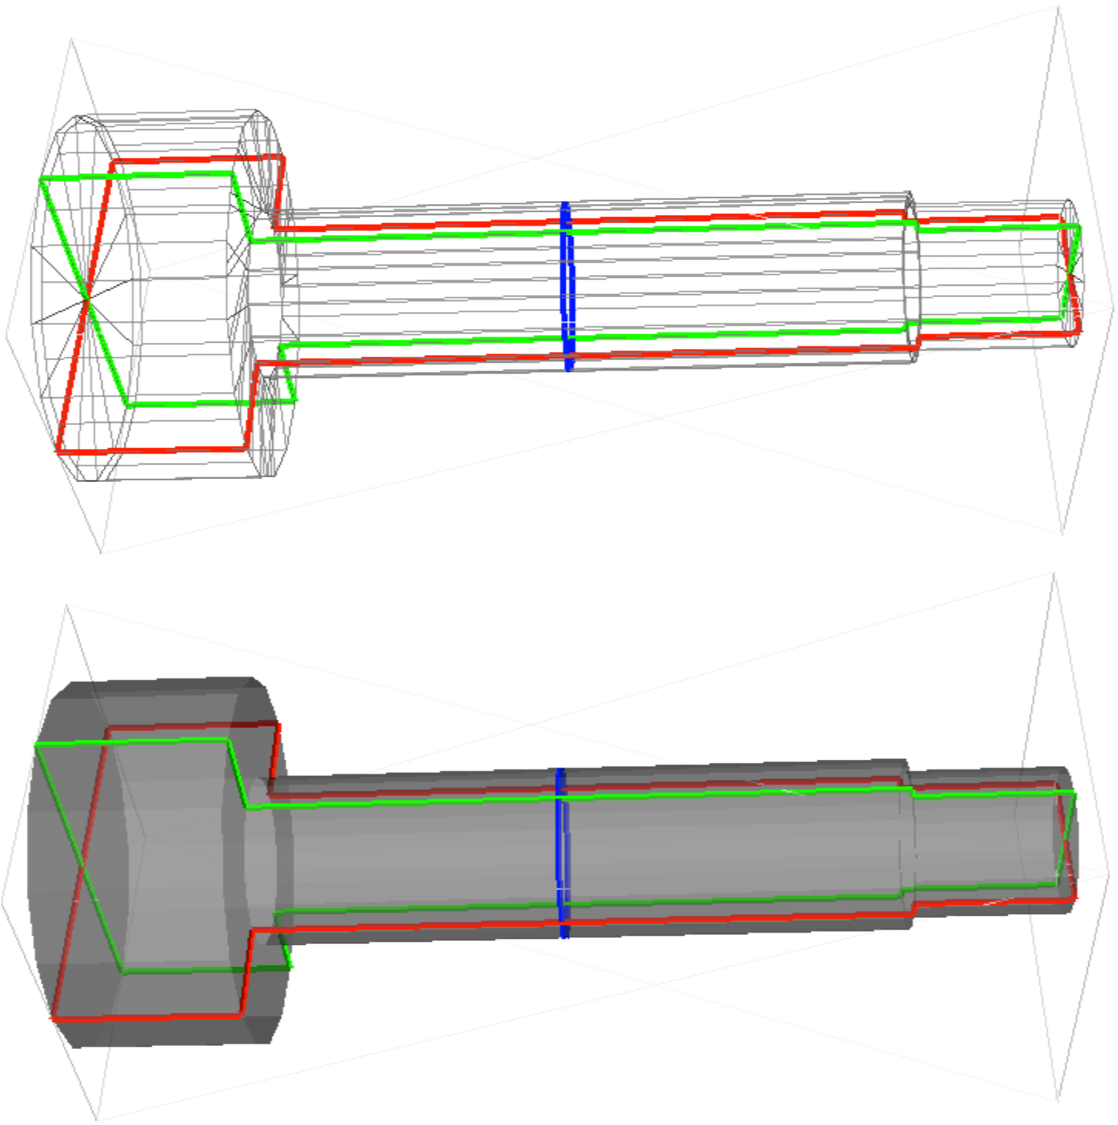
\includegraphics[width=0.9\textwidth]{{Images//CAD_Screw//boltVTK.png}}
  \hspace{5cm}\captionof{figure}{Compound boolean solid recreation of imported CAD model, shown in VTK.}
  \label{boltinvtk}
\end{minipage}%
\end{figure}
\\
\begin{figure}[h!]
\centering
\begin{minipage}{.5\textwidth}
  \centering
  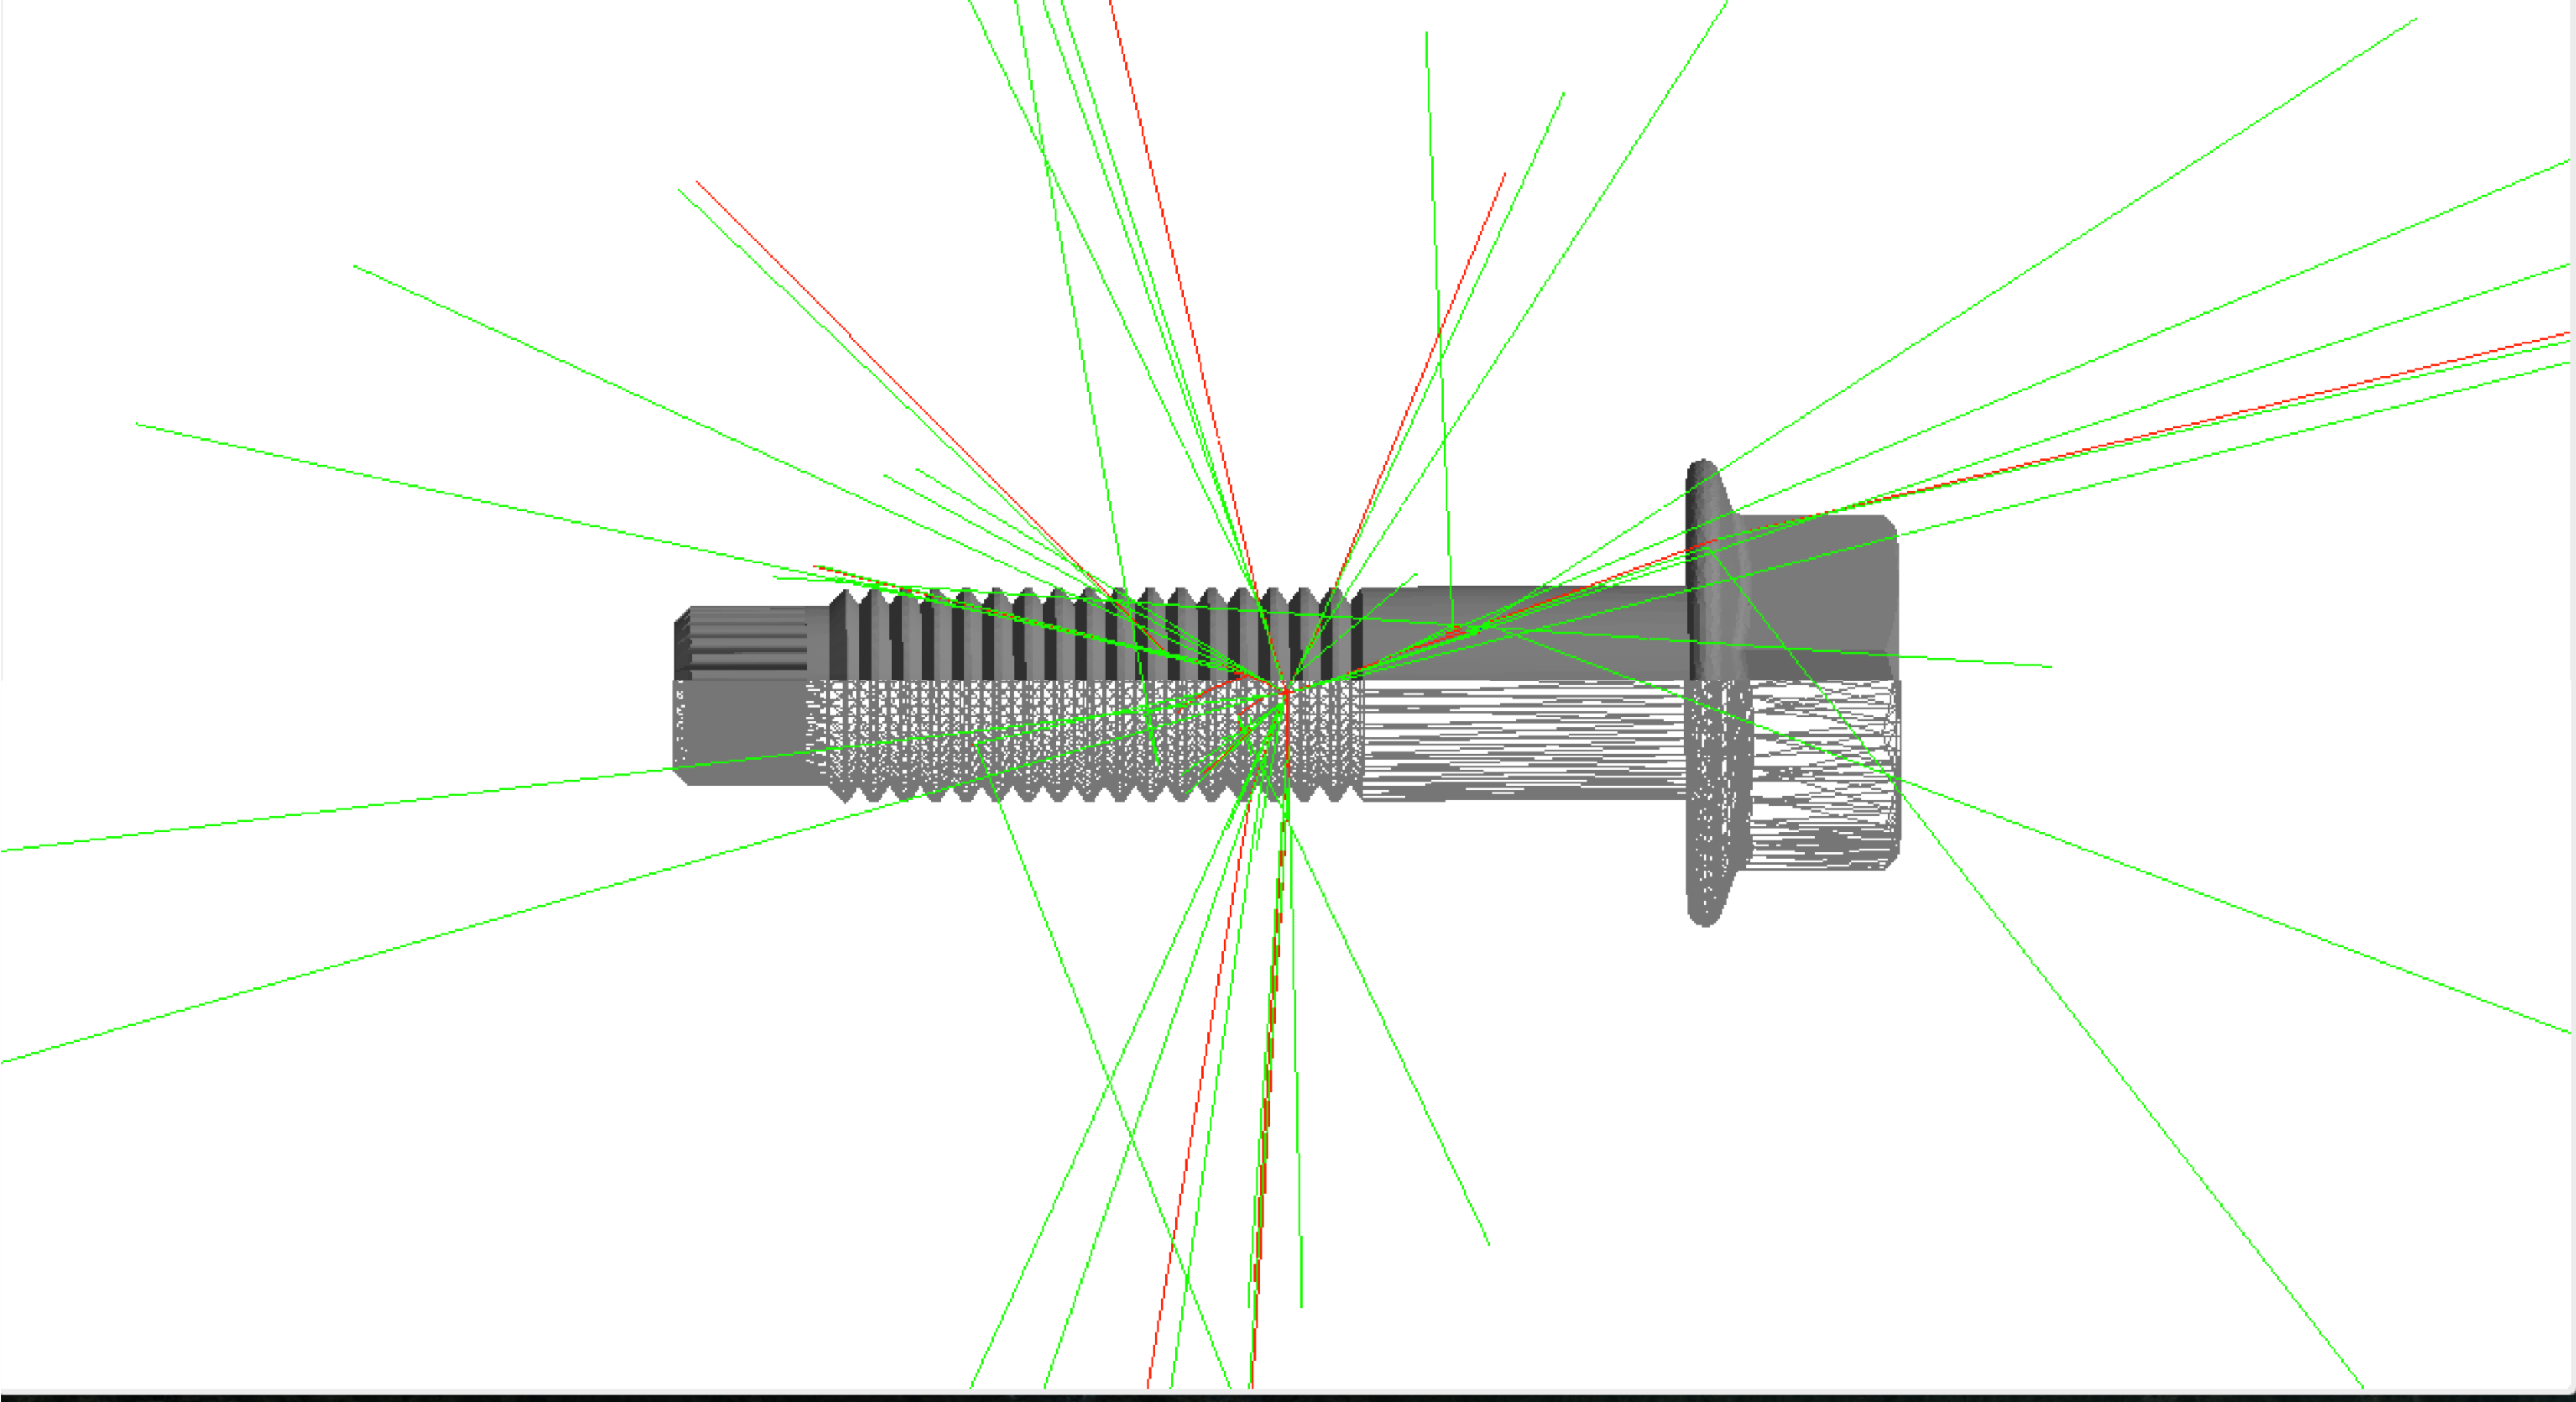
\includegraphics[height=.5\linewidth]{Images//CAD_Screw//Screw_hnh_10MeVe.png}
  \captionof{figure}{A Screenshot of the imported CAD\\ bolt in BDSIM interacting with 10 100 MeV\\ electrons}
  \label{notmybolt}
\end{minipage}%
\begin{minipage}{.5\textwidth}
  \centering
  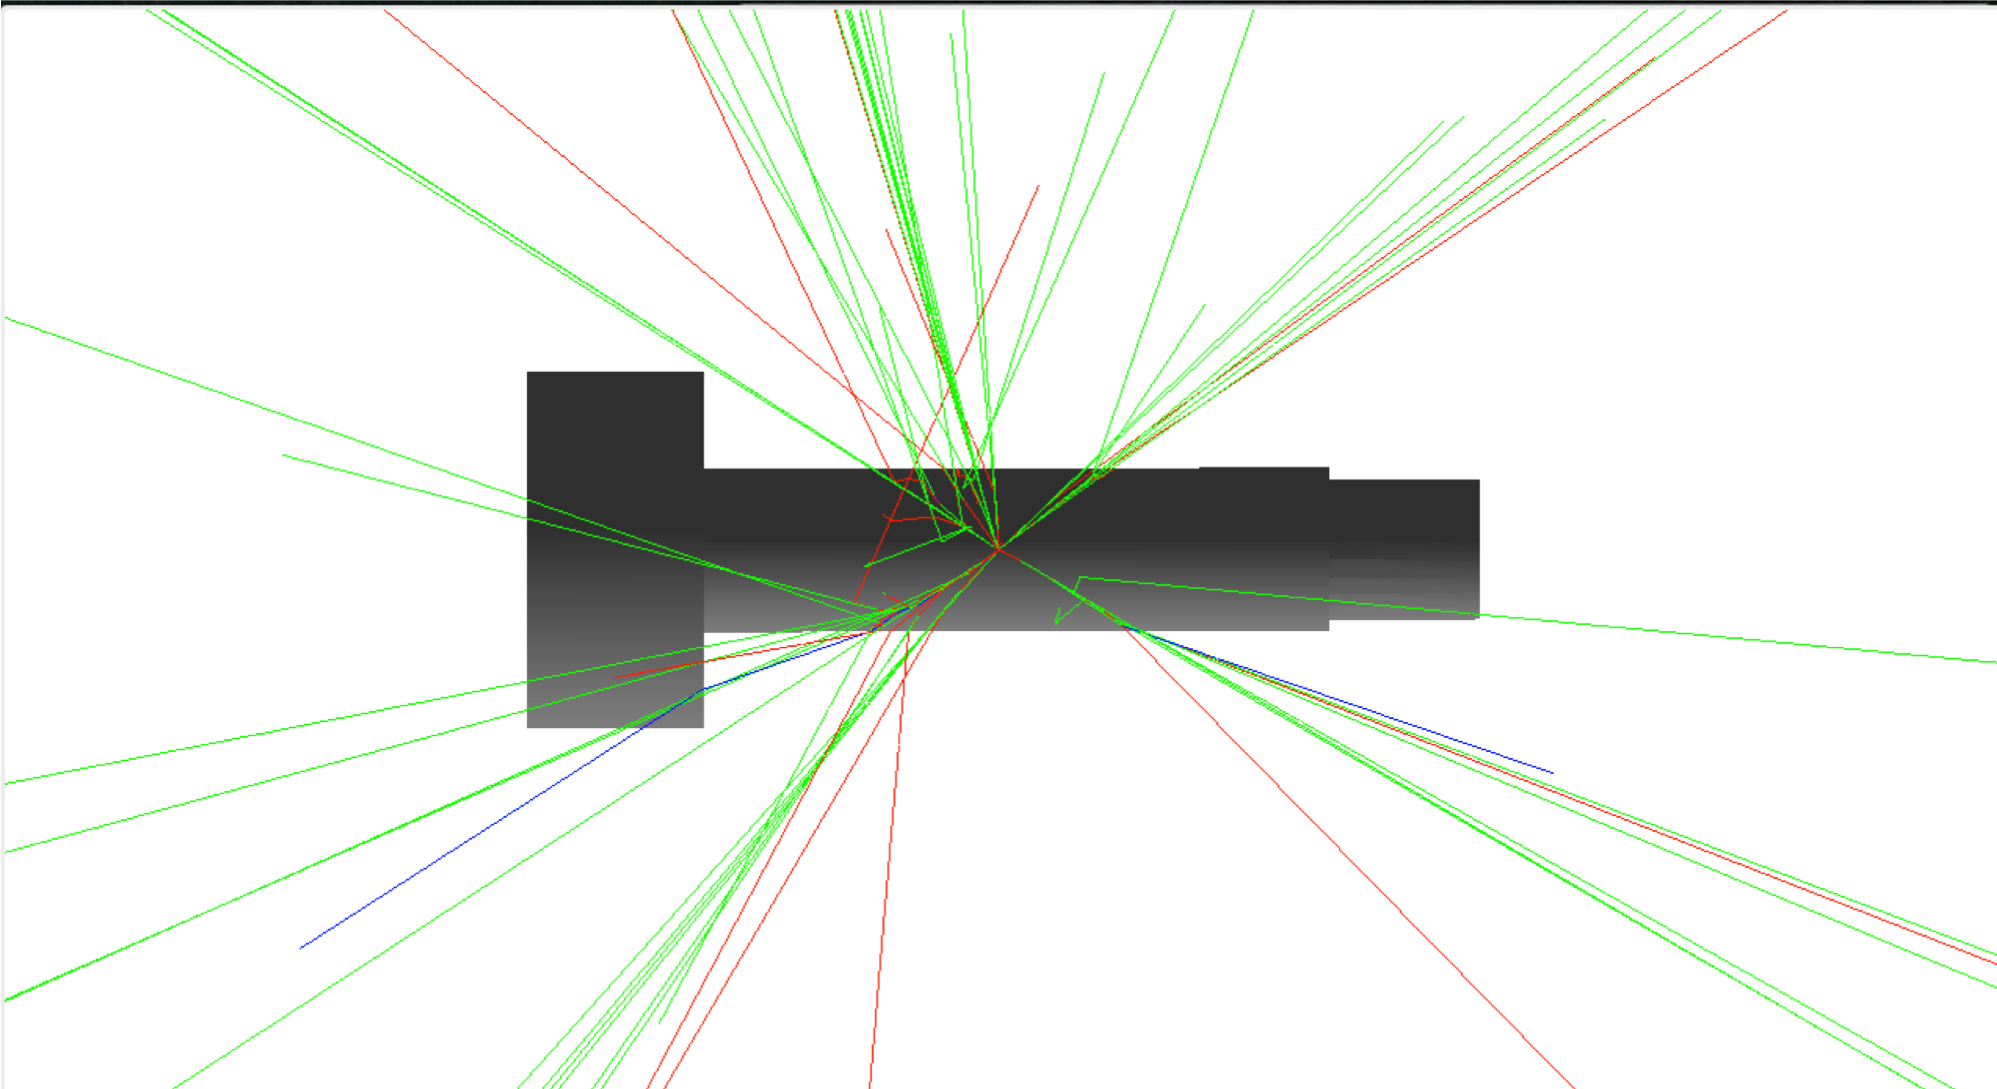
\includegraphics[height=.5\linewidth]{Images//CAD_Screw//bensboltinbdsim.png}
  \captionof{figure}{A Screenshot of the boolean CAD\\ bolt in BDSIM interacting with 10 100 MeV\\ electrons}
  \label{mybolt}
\end{minipage}%
\end{figure}
\\
\begin{figure}[h!]
\centering
\begin{minipage}{.5\textwidth}
  \centering
  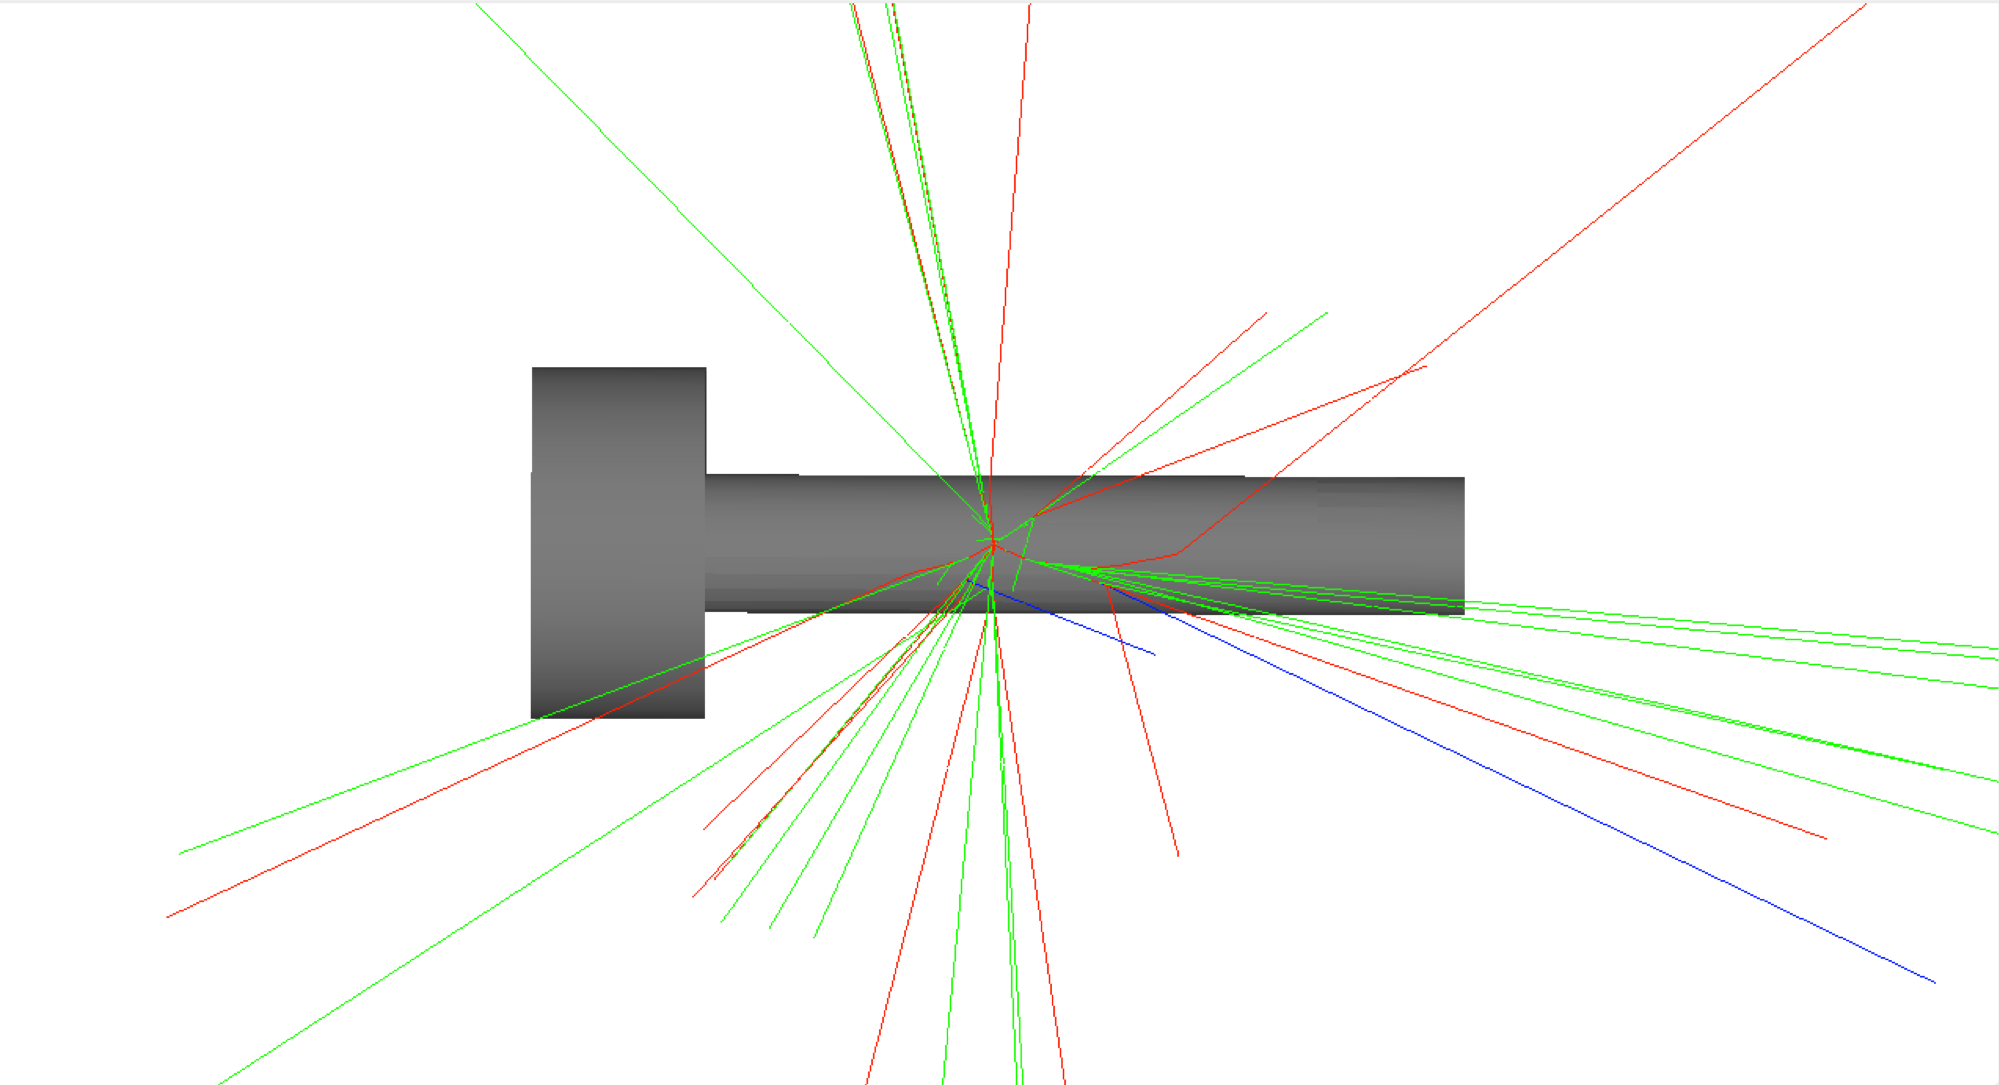
\includegraphics[height=.5\linewidth]{Images//CAD_Screw//skinnybolt.png}
  \captionof{figure}{A Screenshot of the boolean CAD\\ bolt with a reduced body radius in BDSIM\\ interacting with 10 100 MeV electrons}
  \label{mybolt2}
\end{minipage}%
\begin{minipage}{.5\textwidth}
%\begin{table}
\centering
\begin{tabular}{|l|}
\hline
Seeds \\ \hline
1581002619\\ \hline
7538262927\\ \hline
2549647824\\ \hline
\end{tabular}
\vspace{1.6cm}
\captionof{table}{A table showing the values seed values used in Figures \ref{boltcount} \& \ref{boltcountlog}.}
\label{tabbb}
%\end{table}
\end{minipage}%
\end{figure}
\\
\noindent Both bolts were then ran in BDSIM interacting with a batch of 10,000 electrons through a range of energies 1 MeV to 0.75 TeV. The interactions were simulated using the spherical beam distribution origined at the centre of each bolt, as shown in Figure \ref{notmybolt} \& Figure \ref{mybolt} (same method that was used for Spheres in Section \ref{bdsim}). Figure \ref{boltcount} shows the average number of tracks produced from 3 different runs, using a set seed for each run, for both the boolean and CAD bolts. The seeds averaged across can be seen in Table 3. The number of tracks is calculated by subtracting the 10,000 tracks made by the initial electrons from the total number of particle tracks extracted using Pybdsim (Section\ref{pyb}) in each run.
\\
\begin{figure}[h!]
\centering
\begin{minipage}{.5\textwidth}
  \centering
  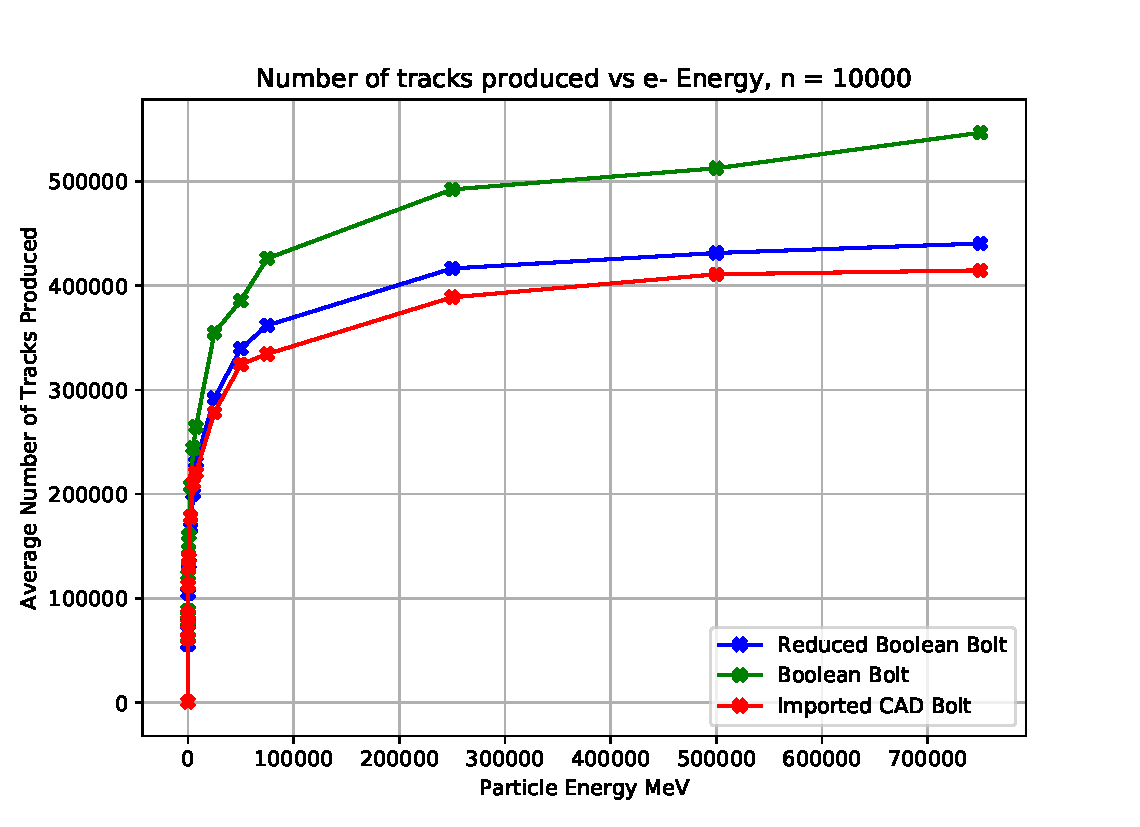
\includegraphics[width=1.05\textwidth]{Images//CAD_Screw//allcount.pdf}
  \captionof{figure}{The average number of particles\\
   tracks produced in BDSIM when interacting\\ 10,000 electrons of increasing energies from\\ different GDML targets.}
  \label{boltcount}
\end{minipage}%
\begin{minipage}{.5\textwidth}
  \centering
  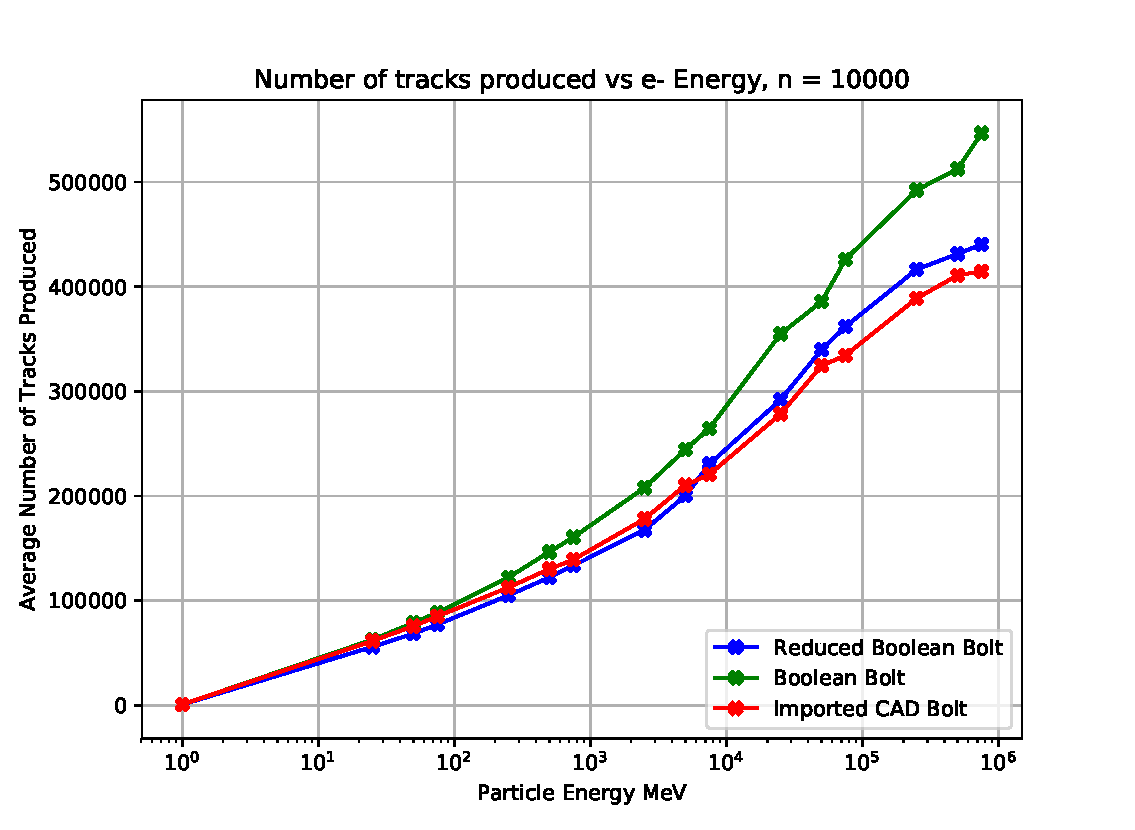
\includegraphics[width=1.05\textwidth]{Images//CAD_Screw//allcoutlog.pdf}
  \captionof{figure}{The average number of particles\\
   tracks produced in BDSIM when interacting 10,000 electrons of increasing energies from different GDML targets with a logarithmic x-axis scale.}
  \label{boltcountlog}
\end{minipage}%
\end{figure}
\\\\
\noindent It can be seen that as the energy is increased the electron interactions generate more secondary particles causing the increase in tracks stored by BDSIM. The gradient of the data begins to flatten out in the range of 200,000 MeV (200 GeV). This flattening is due to the interactions resulting in showers of secondary particles which occur earlier and earlier as the particle energy is increased. Theoretically the graph will then begin to have small drop back down due to the reaction happening near instantaneously. However due to time constraints and the purpose of the plot being to find the energy range where the number of secondary particles is at a sufficiently high amount to generate a histogram of the CPU duration distribution, this range was not explored.
\\\\
\noindent The reason for the number of secondaries is consistently larger for the boolean constructed bolt (Boolean Bolt) compared with the imported CAD bolt (Imported CAD Bolt), is due to the boolean construction being an overestimation of the imported bolt. The overestimation is because of boolean bolt not taking the threads on the bolt into account as well as ignoring hexagonal and cone features on the head of the bolt. This is proven by the creation of a third bolt in which the body of the screw is reduced to a constant 12 [mm] (Figure \ref{mybolt2}. The data for the reduced bolt is plotted in blue and is a much closer to fit to that of the imported CAD than the original boolean replica, which is shown in green in Figure \ref{boltcount}. Figure \ref{boltcountlog} is the same plot as Figure \ref{boltcount}, but has a logarithmic scale for energy. It can be seen that despite the reduction in the size of the bolt it is still an over estimation of the imported CAD model. 
\\
\begin{figure}[h!]
\centering
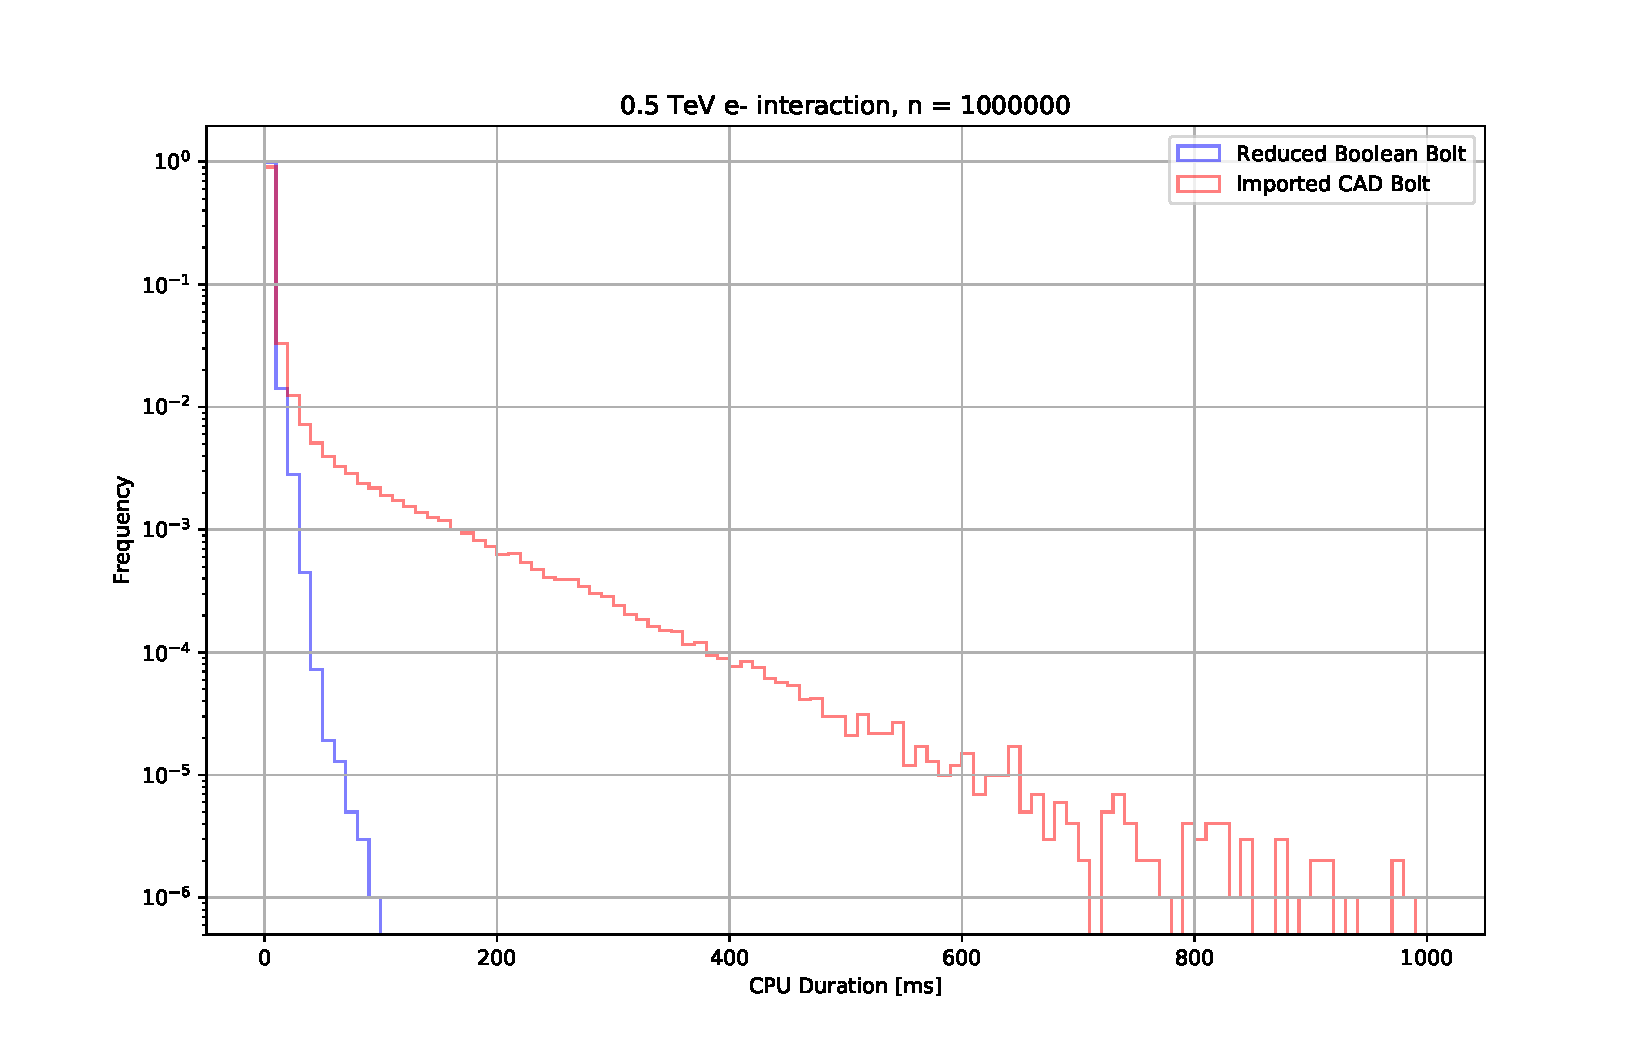
\includegraphics[scale=0.5]{Images//CAD_Screw//boltdist.pdf}
\caption[width=\columnwidth]{CPU duration distribution of 1,000,000 0.5 TeV electrons interacting with CAD models of a bolt.}
\label{lastplot}
\end{figure}
\\
\noindent Simulations of interactions with both CAD models were then repeated with 1,000,000 electrons at an energy at 0.5 TeV. The CPU duration distributions can be seen in Figure \ref{lastplot}. The seed used for both Figure \ref{lastplot} and Figure \ref{vcdist} was 1581002619. The binning of the histograms was set to be 100 bins across the range of 0 to 1000 [ms], it was originally planned to run the simulations a few times at different seed values to create an average. However as seen in Figure \ref{lastplot} the imported CAD bolt took significantly long to simulate. The reason the CAD bolt has a much longer CPU duration than the reduced boolean constructed bolt is due to the increased complexity of the geometric mesh, which creates more sporadic particle tracks.
\\
\begin{figure}[h!]
\centering
\begin{minipage}{.5\textwidth}
  \centering
  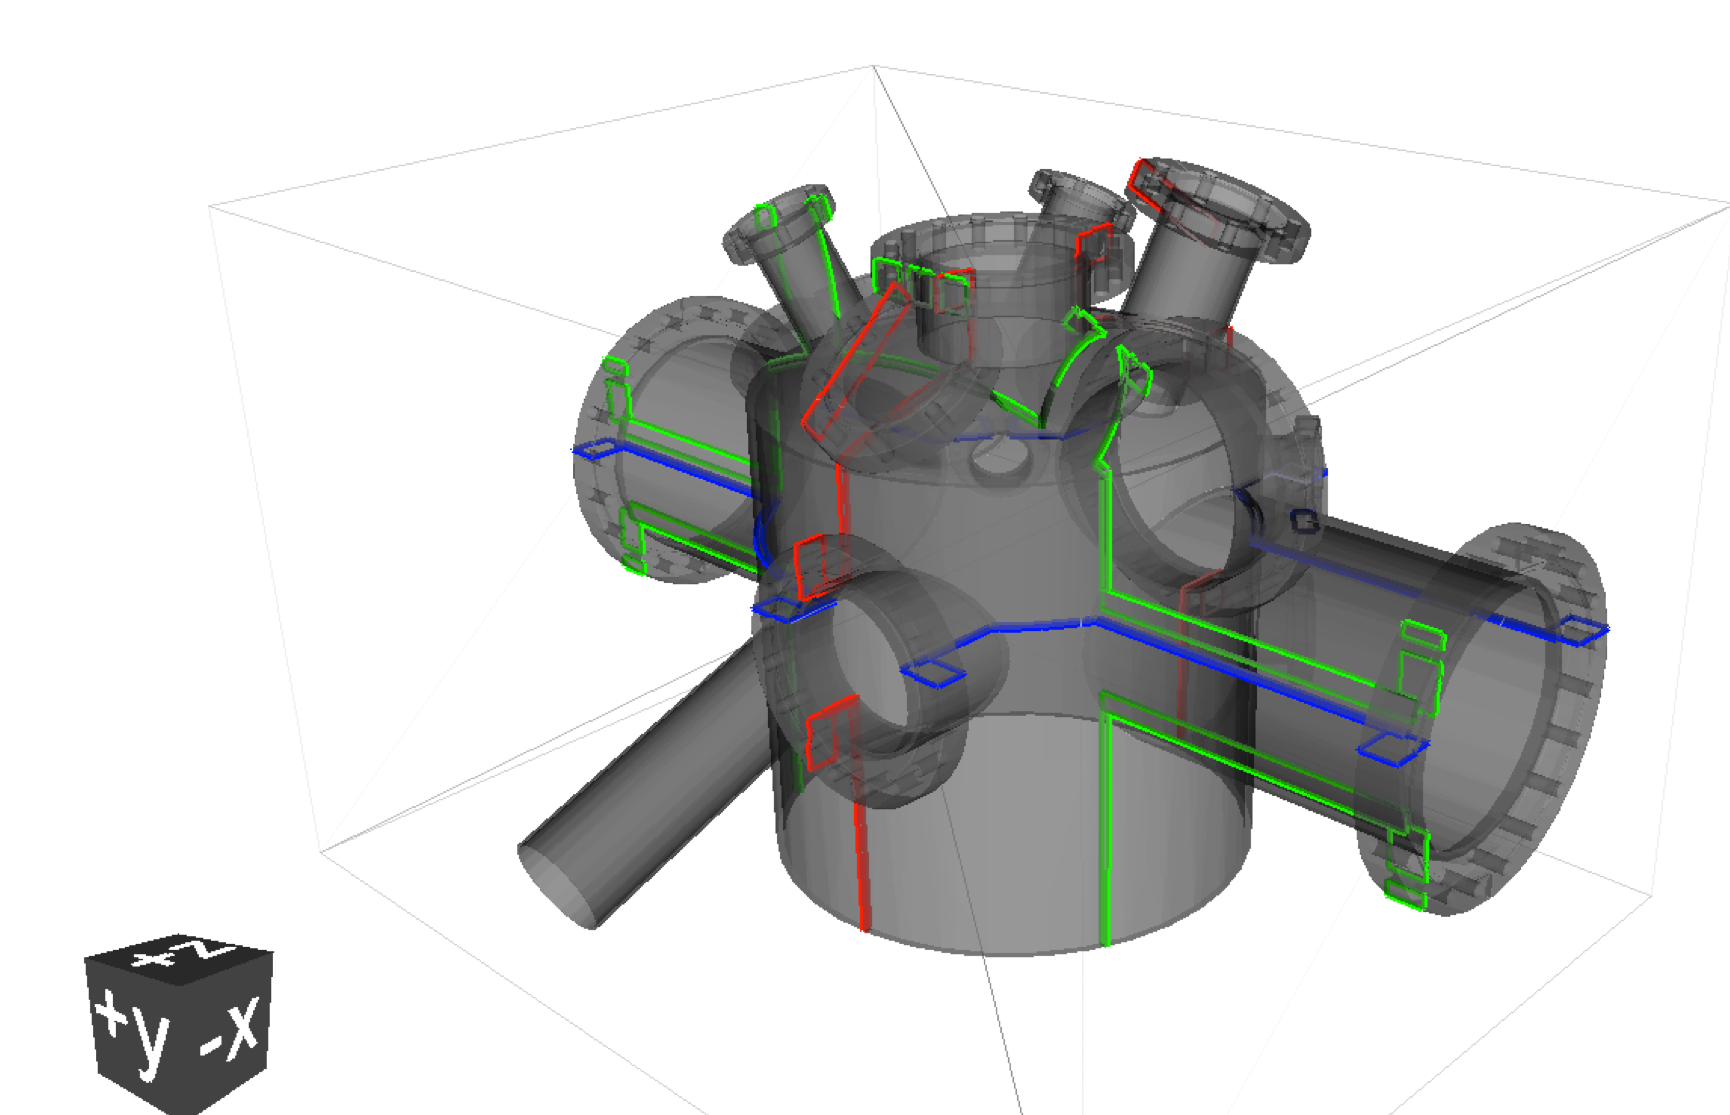
\includegraphics[height=0.5\linewidth]{Images//VC//VC1.png}
  \captionof{figure}{A VTK screenshot of the\\ imported CAD vacuum chamber}
  \label{vcvtk}
\end{minipage}%
\begin{minipage}{.5\textwidth}
  \centering
  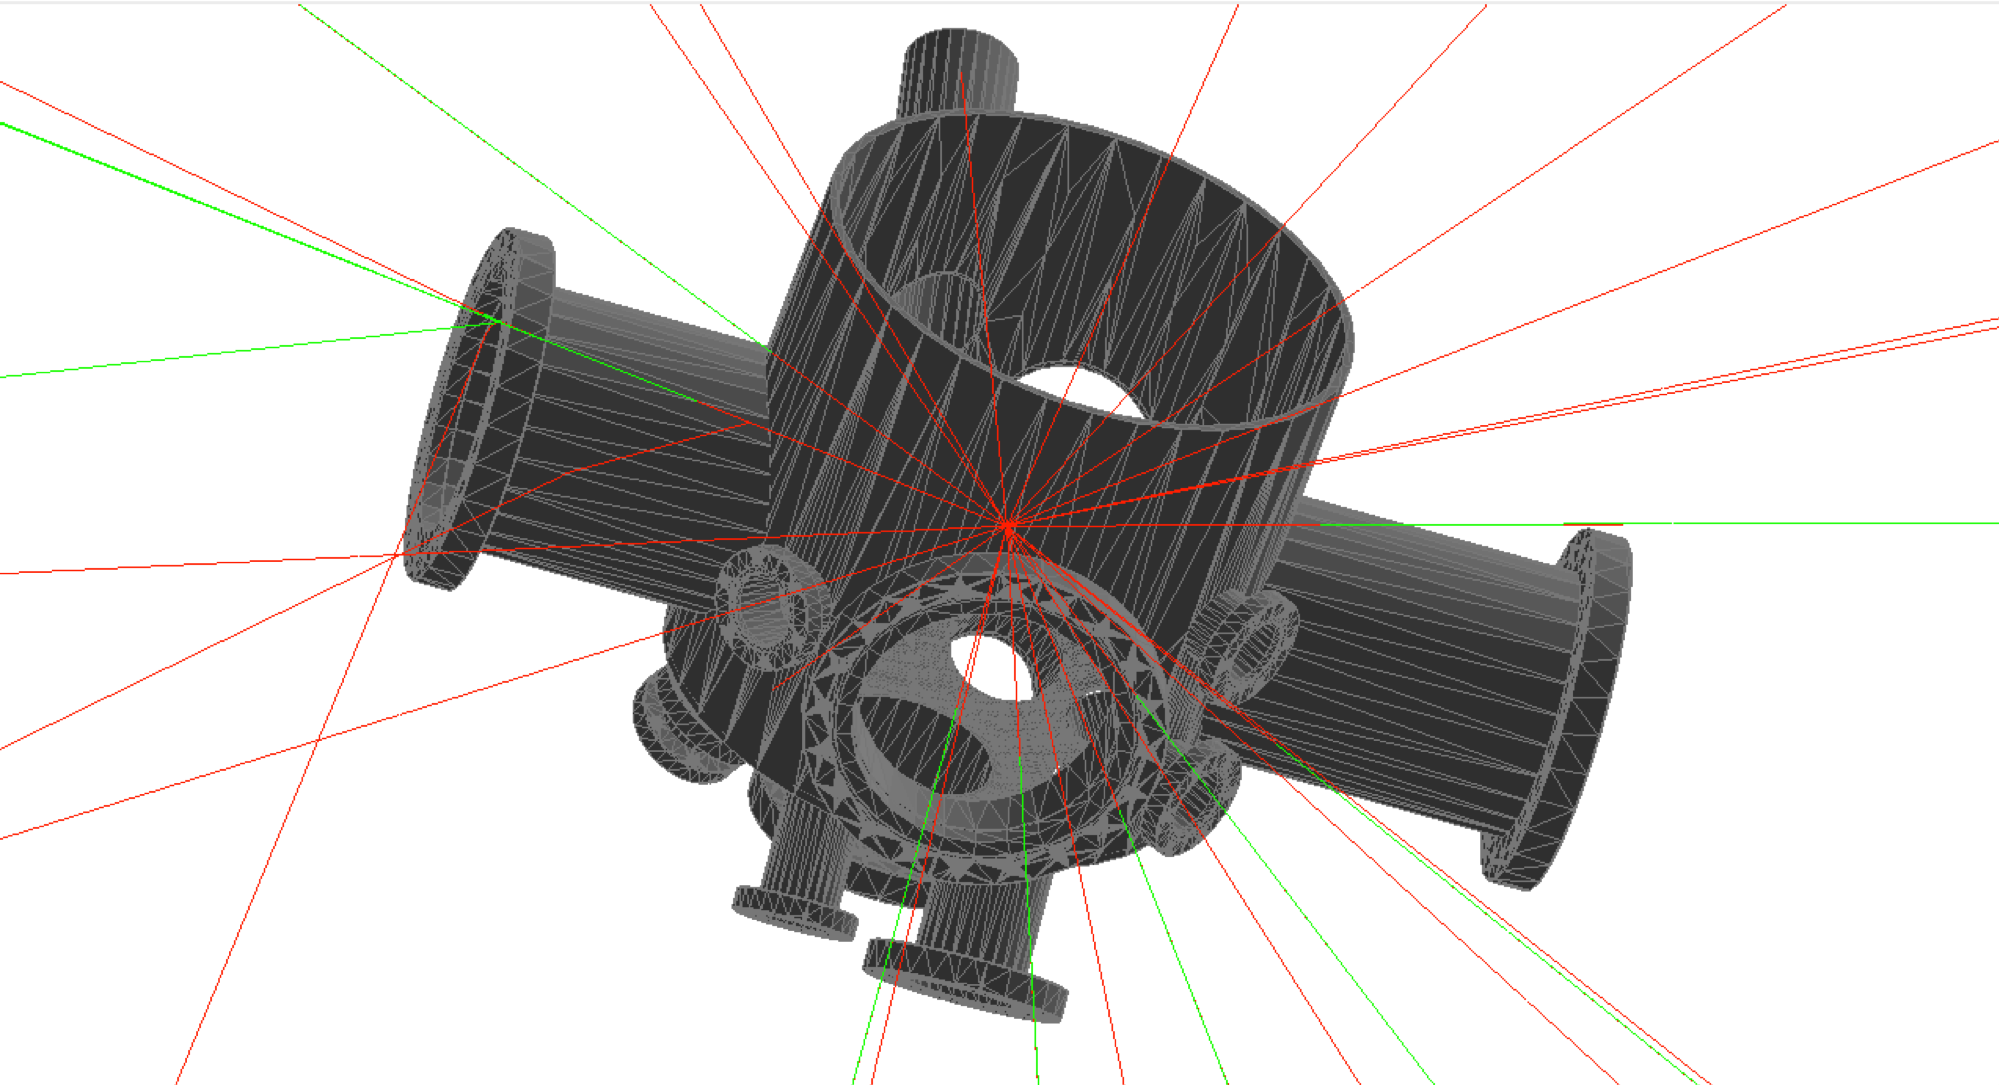
\includegraphics[height=0.5\linewidth]{Images//VC//VC4.png}
  \captionof{figure}{A BDSIM screenshot of the\\ imported CAD vacuum chamber}
  \label{vcbdsim}
\end{minipage}%
\end{figure}
\\
Fortunately there was enough time to run the same analysis for a much more complex CAD model, Figure \ref{vcvtk} shows the imported CAD model of a vacuum chamber imported into Pyg4ometry and downloaded from source \cite{vc}. The model was put through the same process as the previous CAD bolt, being converted from a STEP file to a GDML format with a material of G4\_STAINLESS-STEEL (which is a typical material for a vacuum chamber container). The CAD model of the vacuum chamber was put through the same analysis as the previous CAD bolt, being simulated interacting with electrons in BDSIM on increasing particle energy whilst counting the number of tracks. Figure \ref{vcbdsim}, shows the imported CAD model of the vacuum chamber in BDSIM interacting with 25 100 MeV electrons. 
\\
\begin{figure}[h!]
\centering
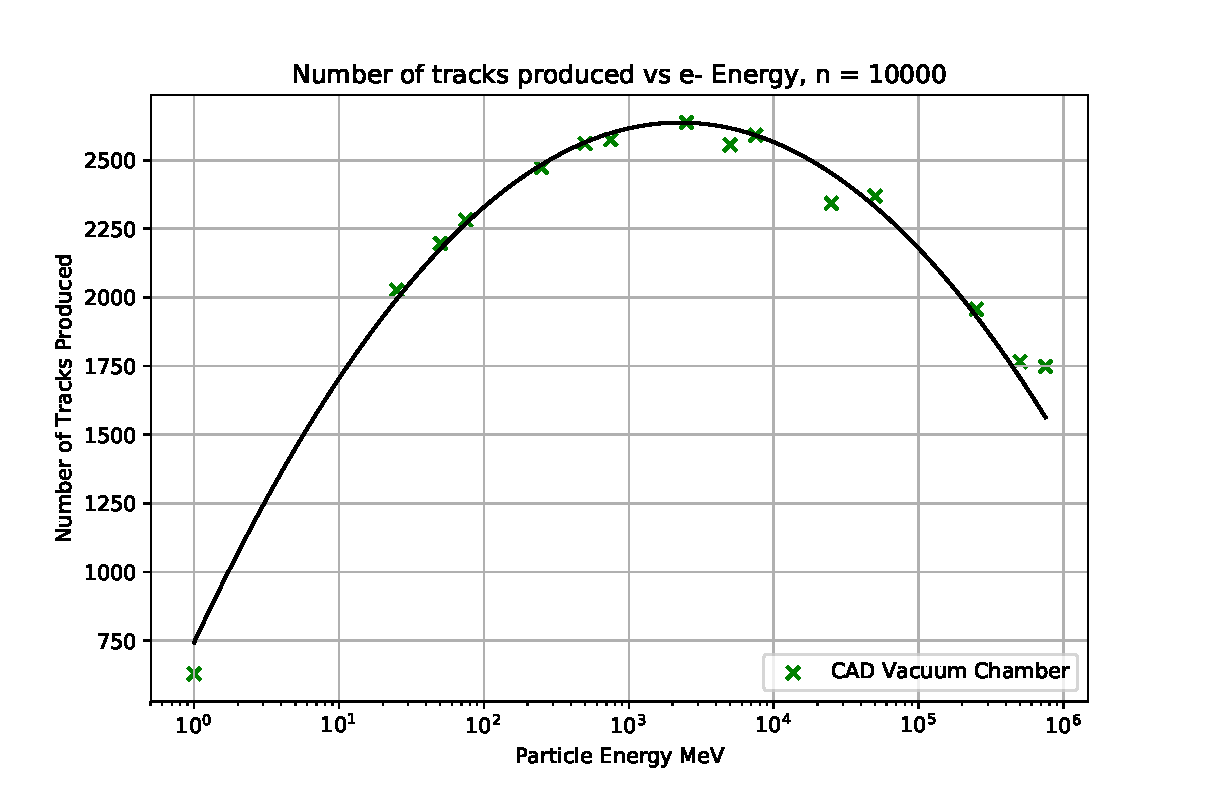
\includegraphics[scale=0.5]{Images//VC//countvclogfinal.pdf}
\caption[width=\columnwidth]{Number of tracks produced in a BDSIM simulated interaction between electron of vary energies and a CAD model of a vacuum chamber.}
\label{vccount}
\end{figure}
\\
\begin{figure}[h!]
\centering
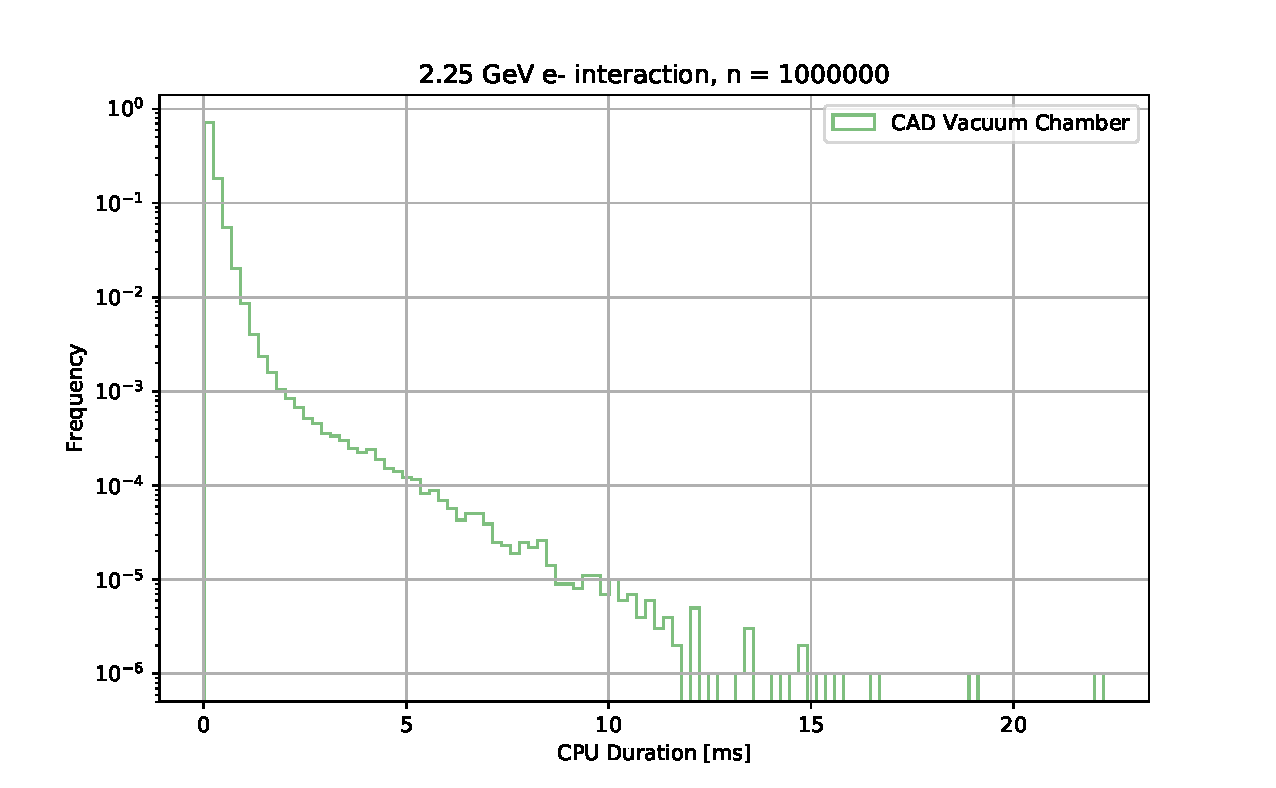
\includegraphics[scale=0.5]{Images//VC//vcdist.pdf}
\caption[width=\columnwidth]{Histogram showing the CPU duration distribution of a BDSIM interaction with 1,000,000 2.25 GeV electrons.}
\label{vcdist}
\end{figure}
\\\
\noindent Figure \ref{vccount} shows the relationship number of tracks produced as the electron energy in increased. The electrons were simulated using the spherical distribution as before, with placement at the centre of the vacuum chamber and a world material of vacuum. This time a clear quadratic relationship can be seen. In which a fit can be applied, the fit gave an energy of 2246.31207496 MeV at a peak number of particles equal to 2637. The peak energy value is then used as the electron energy for Figure \ref{vcdist}. The parameters for the quadratic fit in Figure \ref{vccount} are displayed in Table \ref{vctab}.
\\
\begin{table}[h!]
\centering
\begin{tabular}{|l|l|}
\hline
Parameter & Value [mm] \\ \hline
$a$ &  -31.80126415\\ \hline
$b$ &  490.80581809\\ \hline
$c$ &  743.39452632\\ \hline
\end{tabular}
\caption{TODO}
\label{vctab}
\end{table}

\section{Conclusion \& Summary}
\label{conc}

\subsection{Improvements \& Observations}

The majority of improvements in the project resulted from the rewriting of the tessellated curved primitive solid meshing scripts in Pyg4ometry (Section \ref{pyg}). The new scripts were proven to be computationally more efficient and even produce mesh structures that were aesthetically neater. This was primarily down to the removal of dependence on boolean operations within in the pycsgmesh functions and replacing them with co-ordinate system specified adapted trigonometry that uses both quadrilateral and triangular faces for tessellation. The full raw results for each solid can be entirely viewed in Appendix \ref{app1}. The results clearly show that the number of polygonal faces on a mesh increases much more uniformly gradual as the mesh density is increased. Subsequently the computation needed to create a given mesh exhibits the same relationship, as the CPU time of the meshing scripts scales with the number of faces on that particular solid. This is also increases the time taken to convert and import a meshed solid to GDML format and in to a BDSIM environment as they mesh much cleaner in structure with less points to process. 
\\\\
Other observations made throughout the duration of the project were factors such as the effects of stopping power of target materials on a simulation. The ability to factor out materials when simulating interactions with spherical shapes can be utilised by scaling the radii by the respective stopping distance. The main driving factor for the properties of CPU duration distributions of interactions is governed by the energy of the incident particle/s and the number of particles in a given event. The more initial particles the smoother the distribution as there is a larger data set, as well as a small increase in the width due to a higher number of events 

\subsection{Applications}
As discussed in the introduction (Section \ref{back}) there are many invaluable uses for software packages such as BDSIM and Pyg4ometry that can be used to aid not only the scientific research community of particle physicist, but also help everyday people by improving medical treatment and space exploration. Thanks to the software being open-source and their wide range of compatible files it can be used to simulate a growing number of projects. This comes from the help of a lot of prerequisites such the to GEANT4 databases and Monte Carlo calculations.

\subsection{Project Extensions}
If given more time there is several things that I  would have wished to pursue in addition to the project. One being that the analysis done on a Sphere in Section \ref{bdsim} to also be performed on every one of the remeshed curved primitive solids, all of which are listed in the Appendix \ref{ap1}. This way you could have gain an even more complete picture of the improvement to the meshing of compound solids. Despite a lot of the plots being normalised over a few seed values and being ran with 10,00 of more initial particles, the simulations could be re reran with a more particles and for a larger number of seeds. Another area that could have been explored in more detail is a prototype magnet in which I began to make , can be seen in the Appendix \ref{mag}. As a further analysis of the comparison between the new and old meshing scripts. contour plots could be made to display the variation of both stack and slice for each shape.

\subsection{Acknowledgments}
I would like to say a special thank you to all the Post-docs and PhD students within JAI at Royal Holloway that helped me and made the project that much more enjoyable. Their continuous patience and support always made me feel welcome and equal within the group, and really made me feel apart of the team. Finally I would like to thank my supervisor, Stewart Boogert for overlooking the whole project and constantly pushing me. 
% ------------------------------------------------------------------------------------------------------------------------------

\newpage
\newpage
\footnotesize
\bibliographystyle{IEEEtran}
\bibliography{IEEEabrv,library}

% ------------------------------------------------------------------------------------------------------------------------------
\normalsize
\appendix
\setcounter{figure}{0} 

\section{Prototype FreeCAD Magnet}
\label{mag}
This is the first attempt at a prototype magnet made using FreeCAD GUI (Figure \ref{freee}) and exported as a STEP file, which was then converted to a GDML format with GEANT4 material G4\_Cu using Python. A magnetic field map was then attached onto the shape based on a preset dipole field in BDSIM, in which you can see electrons repelling, as shown in Figure \ref{repel}.

\begin{figure}[h!]
\centering
\begin{minipage}{.5\textwidth}
  \centering
  \includegraphics[height=0.5\linewidth]{Images//CAD_Mag//maginfreeCAD.png}
  \captionof{figure}{FreeCAD screenshot}
  \label{freee}
\end{minipage}%
\begin{minipage}{.5\textwidth}
  \centering
  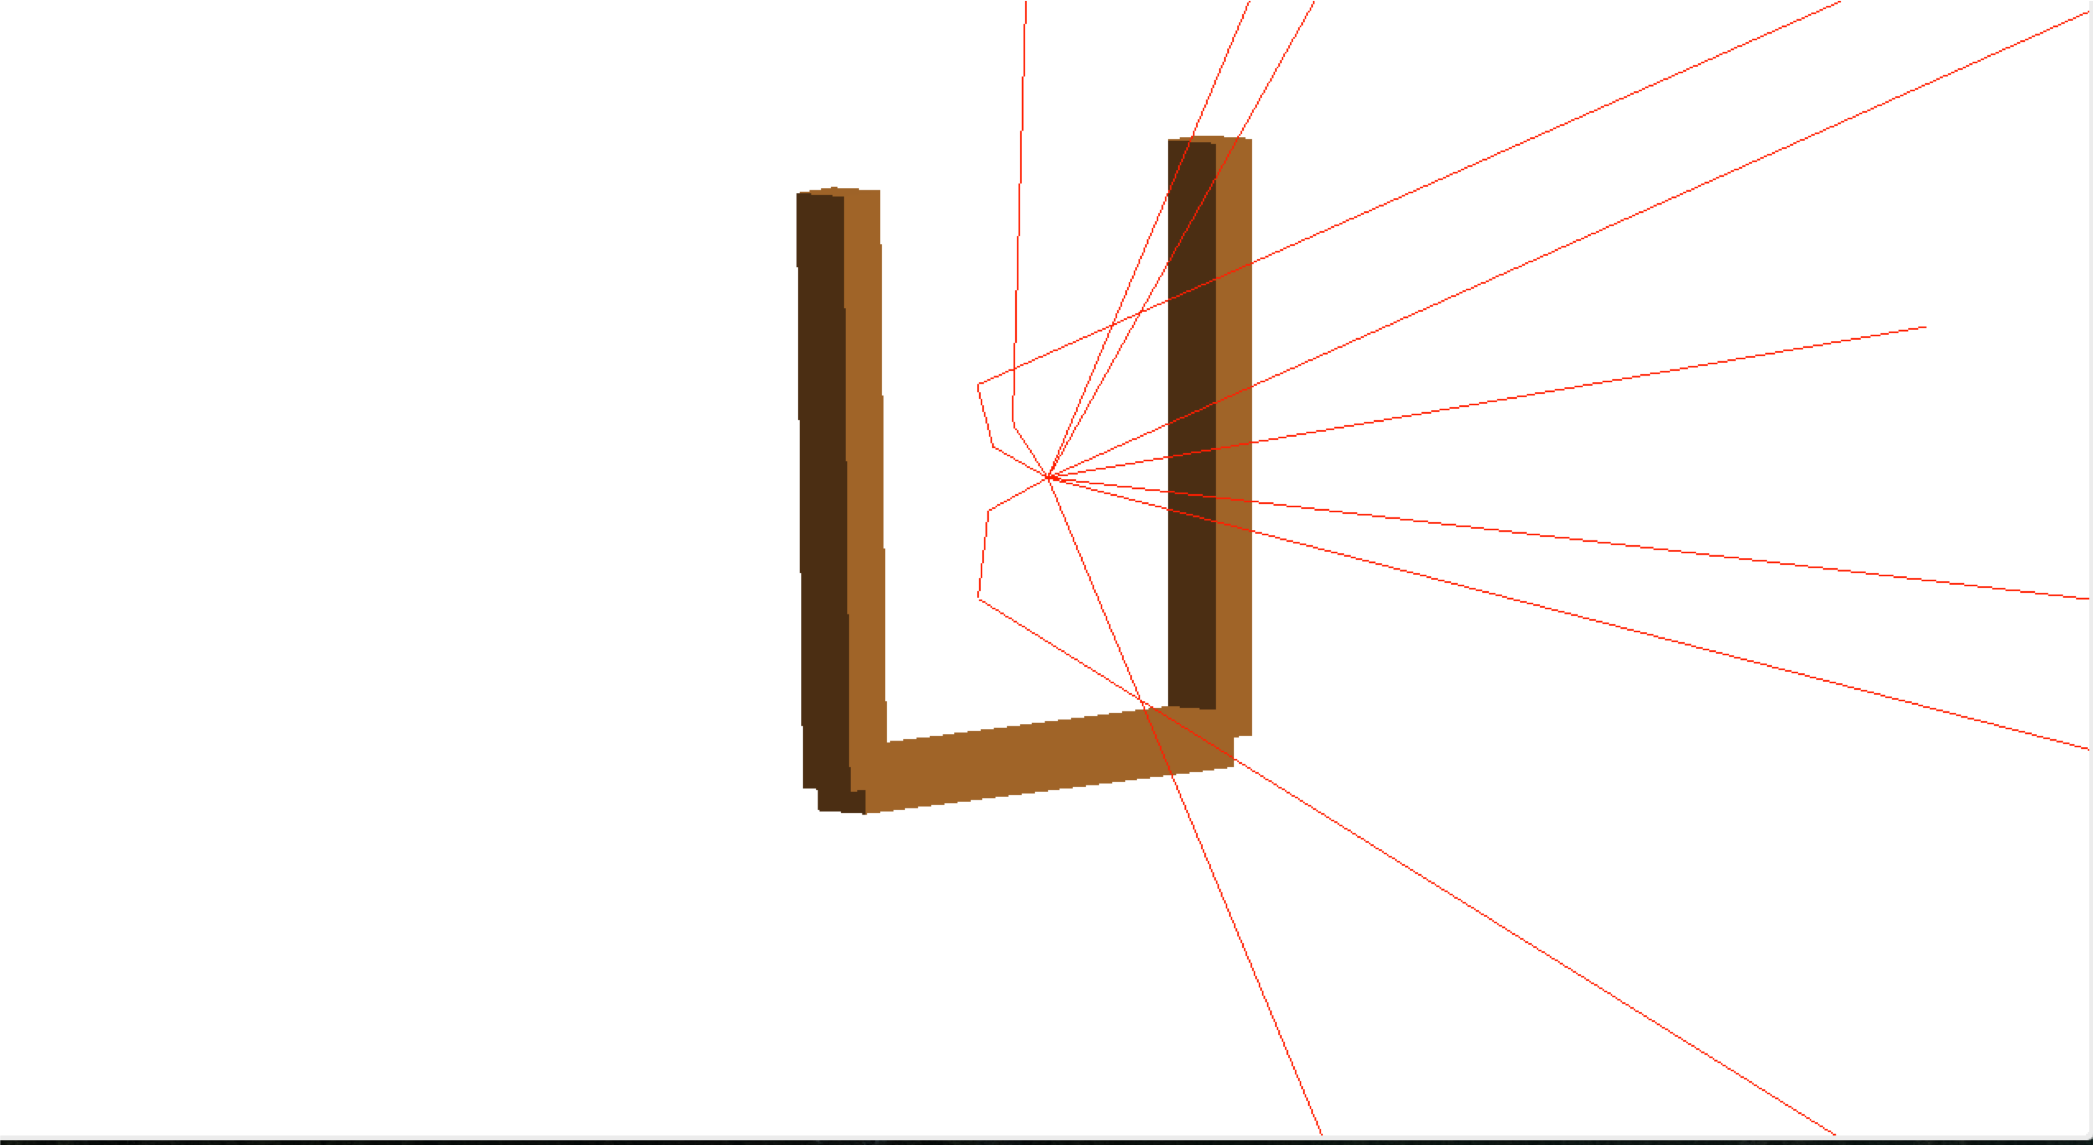
\includegraphics[height=.5\linewidth]{Images//CAD_Mag//maginbdsim.png}
  \captionof{figure}{BDSIM screenshot}
  \label{repel}
\end{minipage}%
\end{figure}

%\newpage
%\subsection{Discovery method contribution pie chart (Figure \ref{pie})}\label{ap2}
%\lstinputlisting[language=Python]{Python//pi.py}
\newpage
\small
\label{appendixstart}
\twocolumn[\section{All Meshed Solids and Polygon Count Plots}
\label{app1}
\label{poy}
The following Figures are the meshing and polygon data for each primitive solid constructed in Pyg4ometry \ref{pyg}. The first Figure for each solid is a screenshot of the old meshing and new meshing visualized in VTK. They show the before and after of each primitive solid in both solid and meshed view. The second Figures Show the number of polygons and triangles produced on a solid as you increase the slice across a range of 10-100 (if there is a stack it is kept at a constant 10). All plots are made using Python and the sold naming convention is the one used by GEANT4 \ref{g4}\\.]
\begingroup
\subsubsection{Cons}
\begin{figure}[h!]
\centering
\begin{minipage}{.2\textwidth}
  \centering
  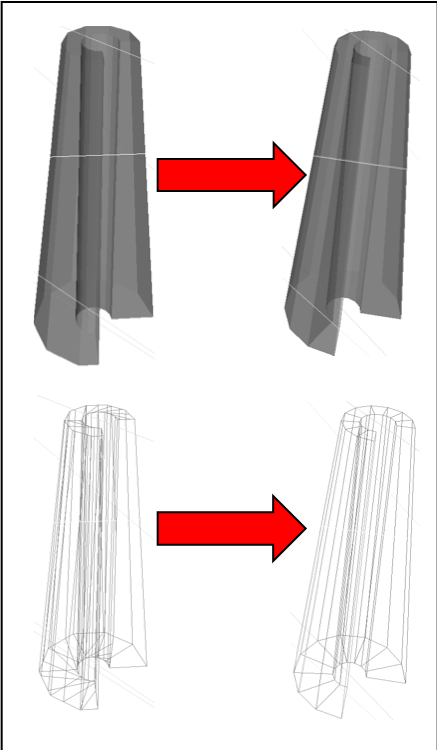
\includegraphics[height=1\linewidth]{Images//Meshes//cons.png}
  \captionof{figure}{}
  \label{cons}
\end{minipage}%
\begin{minipage}{.3\textwidth}
  \centering
  \includegraphics[scale=0.35]{Images//Quad_fits//Cons_quad.pdf}
  \captionof{figure}{ }
  \label{fig:test2}
\end{minipage}%
\end{figure}

\subsubsection{CutTubs}

\begin{figure}[h!]
\centering
\begin{minipage}{.2\textwidth}
  \centering
  \includegraphics[height=1\linewidth]{Images//Meshes//CutTubs.png}
  \captionof{figure}{ }
  \label{ctub}
\end{minipage}%
\begin{minipage}{.3\textwidth}
  \centering
  \includegraphics[scale=0.35]{Images//Quad_fits//CutTubs_quad.pdf}
  \captionof{figure}{ }
  \label{}
\end{minipage}%
\end{figure}
\subsubsection{Ellipsoid}

\begin{figure}[h!]
\centering
\begin{minipage}{.2\textwidth}
  \centering
  \includegraphics[height=1\linewidth]{Images//Meshes//ellipsoid.png}
  \captionof{figure}{ }
  \label{fig:test1}
\end{minipage}%
\begin{minipage}{.3\textwidth}
  \centering
  \includegraphics[scale=0.35]{Images//Quad_fits//Ellipsoid_quad.pdf}
  \captionof{figure}{ }
  \label{fig:test2}
\end{minipage}%
\end{figure}

\newpage
\subsubsection{EllipticalCone}

\begin{figure}[h!]
\centering
\begin{minipage}{.2\textwidth}
  \centering
  \includegraphics[height=1\linewidth]{Images//Meshes//ellipticalcone.png}
  \captionof{figure}{ }
  \label{fig:test1}
\end{minipage}%
\begin{minipage}{.3\textwidth}
  \centering
  \includegraphics[scale=0.35]{Images//Quad_fits//Ellipticalcone_quad.pdf}
  \captionof{figure}{ }
  \label{fig:test2}
\end{minipage}%
\end{figure}

\subsubsection{EllipticalTube}

\begin{figure}[h!]
\centering
\begin{minipage}{.2\textwidth}
  \centering
  \includegraphics[height=0.8\linewidth]{Images//Meshes//ellipticaltube.png}
  \captionof{figure}{ }
  \label{fig:test1}
\end{minipage}%
\begin{minipage}{.3\textwidth}
  \centering
  \includegraphics[scale=0.35]{Images//Quad_fits//EllipticalTube_quad.pdf}
  \captionof{figure}{ }
  \label{fig:test2}
\end{minipage}%
\end{figure}

\subsubsection{Hyperboloid}

\begin{figure}[h!]
\centering
\begin{minipage}{.2\textwidth}
  \centering
  \includegraphics[height=0.9\linewidth]{Images//Meshes//hyperboloid.png}
  \captionof{figure}{ }
  \label{fig:test1}
\end{minipage}%
\begin{minipage}{.3\textwidth}
  \centering
  \includegraphics[scale=0.35]{Images//Quad_fits//Hyperboloid_quad.pdf}
  \captionof{figure}{ }
  \label{fig:test2}
\end{minipage}%
\end{figure}

\newpage
\subsubsection{Orb}

\begin{figure}[h!]
\centering
\begin{minipage}{.2\textwidth}
  \centering
  \includegraphics[height=0.8\linewidth]{Images//Meshes//orb.png}
  \captionof{figure}{ }
  \label{Sphere}
\end{minipage}%
\begin{minipage}{.3\textwidth}
  \centering
  \includegraphics[scale=0.35]{Images//Quad_fits//orb_quad.pdf}
  \captionof{figure}{ }
  \label{fig:test2}
\end{minipage}%
\end{figure}

\subsubsection{Paraboloid}

\begin{figure}[h!]
\centering
\begin{minipage}{.2\textwidth}
  \centering
  \includegraphics[height=1\linewidth]{Images//Meshes//paraboloid.png}
  \captionof{figure}{ }
  \label{para}
\end{minipage}%
\begin{minipage}{.3\textwidth}
  \centering
  \includegraphics[scale=0.35]{Images//Quad_fits//Paraboloid_quad.pdf}
  \captionof{figure}{ }
  \label{fig:test2}
\end{minipage}%
\end{figure}

\subsubsection{Polycone}
\begin{figure}[h!]
\centering
\begin{minipage}{.2\textwidth}
  \centering
  \includegraphics[height=1\linewidth]{Images//Meshes//polycone.png}
  \captionof{figure}{ }
  \label{fig:test1}
\end{minipage}%
\begin{minipage}{.3\textwidth}
  \centering
  \includegraphics[scale=0.35]{Images//Quad_fits//Polycone_quad.pdf}
  \captionof{figure}{ }
  \label{fig:test2}
\end{minipage}%
\end{figure}

\newpage
\subsubsection{Sphere}

\begin{figure}[h!]
\centering
\begin{minipage}{.2\textwidth}
  \centering
  \includegraphics[height=0.75\linewidth]{Images//Meshes//Sphere.png}
  \captionof{figure}{ }
  \label{fig:test1}
\end{minipage}%
\begin{minipage}{.3\textwidth}
  \centering
  \includegraphics[scale=0.35]{Images//Quad_fits//Sphere_quad.pdf}
  \captionof{figure}{ }
  \label{aphh}
\end{minipage}%
\end{figure}

\subsubsection{Torus}

\begin{figure}[h!]
\centering
\begin{minipage}{.2\textwidth}
  \centering
  \includegraphics[height=0.5\linewidth]{Images//Meshes//torus.png}
  \captionof{figure}{ }
  \label{fig:test1}
\end{minipage}%
\begin{minipage}{.3\textwidth}
  \centering
  \includegraphics[scale=0.35]{Images//Quad_fits//Torus_quad.pdf}
  \captionof{figure}{ }
  \label{fig:test2}
\end{minipage}%
\end{figure}

\subsubsection{Tubs}

\begin{figure}[h!]
\centering
\begin{minipage}{.2\textwidth}
  \centering
  \includegraphics[height=0.7\linewidth]{Images//Meshes//tubs.png}
  \captionof{figure}{ }
  \label{fig:test1}
\end{minipage}%
\begin{minipage}{.3\textwidth}
  \centering
  \includegraphics[scale=0.35]{Images//Quad_fits//Tubs_quad.pdf}
  \captionof{figure}{ }
  \label{fig:test2}
\end{minipage}%
\end{figure}

\endgroup
\onecolumn


\section{Appendix (Python scripts)}
\subsection{Sphere BDSIM Vary Mesh Test}
\label{ap1}
\lstinputlisting[language=Python]{Scripts//Run_New_Meshes.py}


\small
%% Table generated by Excel2LaTeX from sheet 'Sheet1'
\begin{table}[htbp]
  \small
  \centering
  \caption{A Table showing the parameters to the quadratic fits for the polygon count plot.}
    \begin{tabular}{lrrrrrr}
    Curved Primitive Solid & \multicolumn{1}{l}{Old a} & \multicolumn{1}{l}{Old b} & \multicolumn{1}{l}{Old c} & \multicolumn{1}{l}{New a} & \multicolumn{1}{l}{New b} & \multicolumn{1}{l}{New c} \\
    Cons  & -2.74E-04 & 3.97E+00 & 5.72E+01 & -3.83E-17 & 4.00E+00 & 2.00E+00 \\
    CutTubs & 2.19E-04 & 5.50E+00 & 6.30E+00 & -3.83E-17 & 4.00E+00 & 2.00E+00 \\
    Ellipsoid & 18.65090372 & -333.5688153 & 1919.792901 & 1.61E-17 & 1.20E+01 & 0.00E+00 \\
    EllipticalCone & 4.00E+00 & 2.00E+00 & 2.41E-12 & 4.03E-18 & 3.00E+00 & 0.00E+00 \\
    EllipticalTube & -1.94E-16 & 4.20E+01 & -5.72E-13 & 4.03E-18 & 3.00E+00 & 0.00E+00 \\
    Hyperboloid & 64.83177713 & -1452.629624 & 16378.18198 & 4.84E-17 & 2.20E+01 & -9.53E-14 \\
    Orb   & -6.45E-17 & 3.40E+01 & -1.91E-13 & -8.06E-18 & 1.00E+01 & -4.77E-14 \\
    Paraboloid & -1.94E-16 & 3.40E+01 & -1.91E-13 & 1.61E-17 & 1.20E+01 & 0.00E+00 \\
    Polycone & 0.39682347 & 7.13011557 & 7.42466252 & -4.03E-17 & 6.00E+00 & 4.00E+00 \\
    Sphere & 10.82154926 & -356.6329124 & 8557.249195 & 2.00E+01 & 2.20E+02 & 1.98E-11 \\
    Torus & 7.01776508 & 304.8746037 & 4899.196225 & -1.61E-17 & 2.00E+01 & -9.53E-14 \\
    Tubs  & 0.27241769 & 4.58191175 & 8.33675211 & -3.83E-17 & 4.00E+00 & 2.00E+00 \\
    \end{tabular}%
  \label{tab1}%
\end{table}
% Table generated by Excel2LaTeX from sheet 'Sheet1'

\newpage
\section{Quadratic Parameters for polygon count plots}
\label{appp1}
The quadratic fit where its parameters are of the form:
\begin{equation}
ax^2 + bx + c = 0
\end{equation}
\begin{table}[h!]
  \small
  \centering
  \caption{A Table showing the parameters to the quadratic fits for the polygon count plot.}
    \begin{tabular}{lrrrrrr}
    Curved Primitive Solid & \multicolumn{1}{l}{$a_{Old}$} & \multicolumn{1}{l}{$b_{Old}$} & \multicolumn{1}{l}{$c_{Old}$} & \multicolumn{1}{l}{$a_{New}$} & \multicolumn{1}{l}{$b_{New}$} & \multicolumn{1}{l}{$c_{New}$} \\
    Cons  & 0.00  & 3.97 & 57.20 & 0.00  & 4.00 & 2.00 \\
    CutTubs & 0.00  & 5.50 & 6.30 & 0.00  & 4.00 & 2.00 \\
    Ellipsoid & 18.65 & -333.56 & 1919.79 & 0.00  & 12.00 & 0.00 \\
    EllipticalCone & 4.00 & 2.00 & 0.00  & 0.00  & 3.00 & 0.00 \\
    EllipticalTube & 0.00  & 42.00 & 0.00  & 0.00  & 3.00 & 0.00 \\
    Hyperboloid & 64.83 & 0.00  & 16378.18 & 0.00  & 22.00 & 0.00  \\
    Orb   & 0.00  & 34.00 & 0.00  & 0.00  & 10.00 & -0.00  \\
    Paraboloid & 0.00  & 34.00 & 0.00  & 0.00 & 12.0 & 0.00 \\
    Polycone & 0.396 & 7.13 & 7.42 & 0.00  & 6.00 & 4.00 \\
    Sphere & 10.82 & -356.63 & 8557.24 & 20.00 & 220.00 & 0.00  \\
    Torus & 7.017 & 304.87 & 4899.19 & 0.00  & 20.00 & 0.00  \\
    Tubs  & 0.27 & 4.581 & 8.33 & 0.00  & 4.00 & 2.00 \\
    \end{tabular}%
  \label{tab1}%
\end{table}



\end{document}